\documentclass[a4paper,oneside,12pt]{book}

%----------------------------------------------------------------------------------------
%	README!
%   Welcome. It's worth having a read through this file
%   to set up the broad parameters, such as the name of
%   the degree, the school/department, the type of work
%   (dissertation/Final Year Project/report, etc. as well
%   as your own details.
%----------------------------------------------------------------------------------------

%----------------------------------------------------------------------------------------
%	COVER PAGE
%   The cover page is laid out in title/title.tex. You can choose a colour
%   or black and white logo
%----------------------------------------------------------------------------------------

%----------------------------------------------------------------------------------------
%	THESIS INFORMATION
%   Put title, author name, supervisor name, degree, type of work, school, department in here
%   It will be used for the title page and for the embedded PDF information
%----------------------------------------------------------------------------------------

%\newcommand{\thesistitle}{Chiral Acoustic Metamaterials for Sound Absorption in the Low-Frequency Range}

\newcommand{\thesistitle}{Quantum-Assisted Optimisation of Secret Key Rate Exchange for UAV Communications using a Rician Channel Model for Physical Layer Security}% Your thesis title, this is used in the title and abstract
\newcommand{\degree}{MEngSc in Electronic \& Computer Engineering} % Replace with your degree name, this is used in the title page and abstract
\newcommand{\typeofthesis}{thesis} % dissertation, Final Year Project, report, etc.
\newcommand{\authorname}{Piers Keegan} % Your name, this is used in the title page and PDF stuff
%% Do not put your Student ID in the document, as TCD will not publish
%% documents that contain both your name and your Student ID.
\newcommand{\supervisor}{Assistant Professor Anshu Mukherjee} % replace with the name of your supervisor
%\newcommand{\cosupervisor}{NAME HERE} % replace with the name of your co-supervisor if you have one
\newcommand{\keywords}{POPULATE THIS LATER DON'T FORGET} % Replace with keywords for your thesis
\newcommand{\school}{\href{https://www.ucd.ie/eleceng/}{School of Electrical \& Electronic Engineering}} % Your school's name and URL, this is used in the title page
%Edited by HS for engineering

%% Comment out the next line if you don't want a department to appear
%\newcommand{\department}{\href{http://researchgroup.university.com}{Department Name}} % Your research group's name and URL, this is used in the title page


%% Language and font encodings
\usepackage[T1]{fontenc} 
\usepackage[utf8]{inputenc}
\usepackage[english]{babel}

%% Bibliographical stuff
\usepackage[]{cite}
%% Document size
% include showframe as an option if you want to see the boxes
\usepackage[a4paper,top=2.54cm,bottom=2.54cm,left=2.54cm,right=2.54cm,headheight=16pt]{geometry}
\setlength{\marginparwidth}{2cm}
%% Useful packages
\usepackage{amsmath}
\usepackage{amsfonts}
\usepackage[autostyle=true]{csquotes} % Required to generate language-dependent quotes in the bibliography
\usepackage[pdftex]{graphicx}
\usepackage[colorinlistoftodos]{todonotes}
\usepackage[colorlinks=true, allcolors=black]{hyperref}
\usepackage{hyperxmp}
\usepackage{caption} % if no caption, no colon
\usepackage{sfmath} %use sans-serif in the maths sections too
\usepackage[parfill]{parskip}    % Begin paragraphs with an empty line rather than an indent
\usepackage{setspace} % to permit one-and-a-half or double spacing
\usepackage{enumerate} % fancy enumerations like (i) (ii) or (a) (b) and suchlike
\usepackage{booktabs} % To thicken table lines
\usepackage{fancyhdr}
\usepackage{extramarks}
\usepackage{xcolor} % to get TCD colour on headings
\usepackage{tikz}
\usetikzlibrary{quantikz}
\numberwithin{equation}{chapter} %HS edit for (chapter.equation)
\pagestyle{plain} % Embrace simplicity!

\usepackage{notoccite}
\usepackage{color,soul}

\usepackage{verbatim} %added 09-04-2024

\usepackage{subfigure}

%\usepackage{tikz}
%\usetikzlibrary{quantikz}
%\usetikzlibrary{graphdrawing}
%\usetikzlibrary{graphs}

\usepackage{braket}
\newcommand{\ketbra}[2]{\ket{#1}\bra{#2}}

\usepackage[toc]{glossaries}

\usepackage[utf8]{inputenc}

\usepackage{array}

\definecolor{tcd_blue}{RGB}{5, 105, 185}

%% It's personal taste but...
%% Uncomment the following block if you want your name and ID at the top of
%% (almost) every page.

\pagestyle{fancy}
\fancyhf{} % sets both header and footer to nothing
\renewcommand{\headrulewidth}{1pt}
\cfoot{\thepage}
%\ifdefined\authorid
%\lhead{\it \authorname\ (\authorid)}
%\else
%\lhead{\it \authorname}
%\fi

\fancyhead[L]{\nouppercase\leftmark}
\renewcommand{\chaptermark}[1]{\markboth{\thechapter.\ #1}{}}
%\fancyhead[ER,OL]{\thepage}
%% End of block

%% It is good practise to make your font sans-serif to improve the accessibility of your document.  Comment out the following line to disable it (but you really should not)
\renewcommand{\familydefault}{\sfdefault} %use the sans-serif font as default

%% If you insist on not using sans-serif (please don't), consider using Palatino instead of the LaTeX standard
%\usepackage{mathpazo} % Use the Palatino font by default if you prefer it to Computer Modern

%% Format Chapter headings appropriately
\usepackage{titlesec}
\titleformat{\chapter}[hang]{\normalfont\huge\bfseries\color{tcd_blue}}{\thechapter}{1cm}{}{}

\titlespacing*{\chapter}{0pt}{0pt}{0pt}

\title{\thesistitle}
\author{\authorname}


\hypersetup{
   pdftitle=\thesistitle, % Set the PDF's title to your title
   pdfauthor=\authorname, % Set the PDF's author to your name
   pdfkeywords=\keywords, % Set the PDF's keywords to your keywords
   pdfsubject=\degree, % Set the PDF's keywords to your keywords
   pdfinfo={
     pdfsupervisor=\supervisor, % Set the PDF's supervisor to your supervisor
     %pdfcosupervisor=\cosupervisor, % Set the PDF's cosupervisor to your cosupervisor if using
   }
}

\makeglossaries

\newacronym{bs}{BS}{Base Station}
\newacronym{td}{TD}{Terminal Device}
\newacronym{los}{LoS}{Line of Sight}
\newacronym{nlos}{NLoS}{Non-Line of Sight}
\newacronym{masr}{MASR}{Minimum Average Secrecy Rate}
\newacronym{uav}{UAV}{Unmanned Aerial Vehicle}
\newacronym{uavs}{UAVs}{Unmanned Aerial Vehicles}
\newacronym{hap}{HAP}{High-Altitude Platform}
\newacronym{lap}{LAP}{Low-Altitude Platform}
\newacronym{pls}{PLS}{Physical Layer Security}
\newacronym{ue}{UE}{User Equipment}
\newacronym{gu}{GU}{Ground User}
\newacronym{lu}{LU}{Legitimate User}
\newacronym{ofdm}{OFDM}{Orthogonal Frequency Division Multiplexing}
\newacronym{noma}{NOMA}{Non-Orthogonal Multiple Access}
\newacronym{qubo}{QUBO}{Quadratic Unconstrainted Binary Optimisation}
\newacronym{aqc}{AQC}{Adiabatic Quantum Computation}
\newacronym{sca}{SCA}{Successive Convex Approximation}
\newacronym{cps}{CPS}{Cyber-Physical System}
\newacronym{manet}{MANET}{Mobile Ad Hoc Network}
\newacronym{mec}{MEC}{Mobile Edge Computing}
\newacronym{ppo}{PPO}{Proximal Policy Optimisation}
\newacronym{drl}{DRL}{Deep Reinforcement Learning}
\newacronym{cqm}{CQM}{Constrained Quadratic Model}
\newacronym{lqdrl}{LQ-DRL}{Layerwise Quantum Deep Reinforcement Learning}
\newacronym{sinr}{SINR}{Signal to Interference \& Noise Ratio}
\newacronym{snr}{SNR}{Signal to Noise Ratio}
\newacronym{csi}{CSI}{Channel State Information}
\newacronym{marl}{MARL}{Multi-Agent Reinforcement Learning}
\newacronym{qam}{QAM}{Quadrature Amplitude Modulation}
\newacronym{awgn}{AWGN}{Additive White Gaussian Noise}
\newacronym{qos}{QoS}{Quality of Service}
\newacronym{pud}{PUD}{Positive Unique Differences}
\newacronym{dft}{DFT}{Discrete Fourier Transform}
\newacronym{cscg}{CSCG}{Circularly Symmetric Complex Gaussian}
\newacronym{fspl}{FSPL}{Free-Space Pathloss}
\newacronym{mimo}{MIMO}{Multiple-Input Multiple-Output}
\newacronym{sic}{SIC}{Successive Interference Cancellation}
\newacronym{ans}{ANS}{Additive Noise Signature}
\newacronym{mitm}{MitM}{Man in the Middle}
\newacronym{oop}{OOP}{Object-Oriented Programming}
\newacronym{bash}{BASH}{Bourne Again Shell}
\newacronym{rf}{RF}{Radio Frequency}
\newacronym{mer}{MER}{Memory Experience Replay}
\newacronym{per}{PER}{Prioritised Experience Replay}
\newacronym{4g}{4G}{4\textsuperscript{th} Generation Wireless Communication}
\newacronym{5g}{5G}{5\textsuperscript{th} Generation Wireless Communication}
\newacronym{hpc}{HPC}{High Performance Computing}
\newacronym{jit}{JIT}{Just-in-Time}
\newacronym{dqn}{DQN}{Deep Q-Network}
\newacronym{is}{IS}{Importance-Sampling}
\newacronym{tde}{TD-error}{Temporal Difference Error}
\newacronym{ip}{IP}{Internet Protocol}

\frontmatter
\begin{document}
\begin{titlepage}

\center % Center everything on the page

%% All the text parameters should be taken from the start of the main.tex file.
%% You should only alter stuff here if you want to change the layout

\vspace*{\fill}

%----------------------------------------------------------------------------------------
%	TITLE SECTION
%----------------------------------------------------------------------------------------
\makeatletter
\onehalfspacing
{\Large \bfseries \thesistitle}\\[0.5cm] % Title of your document

%----------------------------------------------------------------------------------------
%	AUTHOR SECTION
%----------------------------------------------------------------------------------------

by\\[0.5cm]

\ifdefined\authorid
\authorname\\ % Your name
\authorid\\[2cm] % Your Student ID
\else
\textbf{\authorname}\\[1cm] % Your name
\fi


%----------------------------------------------------------------------------------------
%	TYPE OF THESIS SECTION
%----------------------------------------------------------------------------------------
%\vfill
 A \typeofthesis\ submitted to University College Dublin in partial fulfillment\\of the requirements for the degree of\\
\textbf{\degree}\\
in the College of Engineering \& Architecture
\\[1cm]
%\vfill % Fill the rest of the page with whitespace

%----------------------------------------------------------------------------------------
%	LOGO SECTION
%----------------------------------------------------------------------------------------
%% Choose one of the following -- a colour or black-and-white logo


\includegraphics[height=5cm]{title/University_College_Dublin_logo.svg.png}\\[1cm] 
%\includegraphics[width=12cm]{title/black-stacked-trinity.jpg}\\[1cm] 

\Large \school\\[1.5cm] % Minor heading such as course title
\ifdefined\department
\large \department\\[1cm] % Minor heading such as course title
\fi


%----------------------------------------------------------------------------------------
%	Supervisor SECTION
%----------------------------------------------------------------------------------------

\normalsize \textbf{Head of School}: Professor Peter Kennedy\\
\textbf{Supervisor}: \supervisor\\[1cm] % Their name
\ifdefined\cosupervisor
Cosupervisor: \cosupervisor\\ % Their name
\fi
%\\[1cm]

%----------------------------------------------------------------------------------------
%	DATE SECTION
%----------------------------------------------------------------------------------------

{\large \today}\\[2cm] % Date, change the \today to a set date if you want to be precise

\vspace*{\fill}

\end{titlepage}
\pagenumbering{roman}
\setlength{\belowdisplayskip}{0pt} \setlength{\belowdisplayshortskip}{0pt}
\setlength{\abovedisplayskip}{0pt} \setlength{\abovedisplayshortskip}{0pt}

\clearpage
\phantomsection
%\addcontentsline{toc}{chapter}{Declaration of Authorship}
\chapter*{Declaration of Authorship}
\textbf{Student Name}: Piers Keegan

\textbf{Student Number}: 24284403

\textbf{Project Title}: Quantum-Assisted Optimisation of Secret Key Rate Exchange for UAV Communications using a Rician Channel Model for Physical Layer Security

\textbf{Supervisor}: Dr. Anshu Mukherjee

Plagiarism: the unacknowledged inclusion of another person’s writings or ideas or formally presented
work (including essays, examinations, projects, laboratory presentations). The penalties associated with plagiarism designed to impose sanctions seriousness of University’s commitment to academic integrity.
Ensure that you have read the University’s Briefing for Students on Academic Integrity and
Plagiarism and the UCD Statement, Plagiarism Policy and Procedures, (http://www.ucd.ie/registrar/)

I declare that all of the following are true:

1) I fully understand the definition of plagiarism.

2) I have not plagiarised any part of this project and it is my original work.

3) All material in this report is my own work except where there is clear acknowledgement and appropriate reference to the work of others.

I acknowledge the contribution of the following post-graduate students / post-doctoral fellows /
researchers or technicians to work detailed in this report: N/A.

\vspace{15mm}

\begin{tabular}{@{}p{2.5in}p{2in}p{2in}@{}}
    Signed: 
\includegraphics[width=0.15\textwidth]{figures/cropped_signature_declaration_of_authorship.png} && Date: 15\textsuperscript{th} August, 2025 \\
\end{tabular}

\clearpage
\phantomsection
\addcontentsline{toc}{chapter}{Abstract}
\chapter*{Abstract}
This thesis details the novel application of a quantum-classical hybrid deep reinforcement learning algorithm to maximise the secrecy rate of communication links between an unmanned aerial vehicle acting as an aerial base station and a legitimate ground user that is being subjected to eavesdropping. 
It is shown that the methodology outlined in this thesis successfully solves the joint optimisation problem's objective and its subproblems' objectives. 
The secrecy rate, data exchange rate, energy efficiency and UAV trajectory are shown to consistently converge as intended across a range of simulation episodes, demonstrating the effectiveness of the techniques used for solving joint optimisation problems applied to UAV-enabled wireless communications.

The thesis details the current state-of-the-art research that has been conducted on the topics of airborne wireless communications networks, optimisation of particular parameters related to aerial networking platforms, quantum computing techniques and how they have been applied to optimisation of airborne wireless communication platforms in a variety of ways. 
Different network architectures and platforms are considered and explained. 

The scenario and simulation environment involving a single aerial base station providing coverage to a set of legitimate ground users with terrestrial eavesdroppers is detailed. 
A Rician channel model with a communications model employing non-orthogonal multiple accessing is described. 
The joint optimisation problem and its subproblems are then outlined and mathematically derived. 

The system architecture is described at a high level, followed by a more detailed explanation of its constituent subsystems. 
The software engineering principles and Python implementation of the simulations is explained to convey how the simulations were run and the libraries and frameworks are useful for solving this problem are listed.

From there, the simulation parameters are listed.
The results, displaying convergence and maximisation of the secrecy rate and the convergence of its subproblems are shown and discussed. 
It is noted that for deeper quantum circuits in use within the system, that the performance begins to degrade. 

This thesis concludes by outlining the future work that can be carried out to extend this methodology and system architecture. 
Attention is also paid to work that could be conducted to simulate the system and solve the joint optimisation problem for different scenarios, networking platforms, quantum computing techniques and threat models. 
The impacts and benefits of the future work are explained in their respective subsections. 

%This thesis investigates the use of \acrfull{uavs} as aerial base stations (\acrshort{bs}s) and how to optimise various controllable parameters of \acrshort{uav}-\acrshort{bs} to achieve the maximum level of secrecy for secure communications with legitimate ground users (\acrshort{gu}s) that are being subjected to eavesdropping by terrestrial eavesdroppers.  
%The techniques employed as part of the optimisation algorithms explored in this thesis make use of contemporary hybrid classical and quantum computing methodologies to rapidly and accurately compute the optimal parameters to achieve the optimal level of communication secrecy, accounting for power consumption, UAV clustering, trajectory and others. 

\newpage
\onehalfspacing%\raggedright %\raggedright turns off justification and hyphenation

%\clearpage
%\phantomsection
%\addcontentsline{toc}{chapter}{Acknowledgements}
%\chapter*{Acknowledgements}
%%\section*{\Huge\textcolor{tcd_blue}{Acknowledgements}}
%%\hl{You should acknowledge any help that you have received (for example from technical staff), or input provided by, for example, a company.}
%I would like to acknowledge the guidance and support received throughout the development of this project from my supervisor, Dr. Mukherjee, who provided useful guidance and advice in all of our meetings on how to proceed as well as feedback on my work. 
%
%I would also like to thank the university's Research IT department for my use of the Sonic HPC cluster as I would not have been able to 
%\hl{RESEARCH IT GROUP FOR HPC ACCESS, ETC}
%
%\hl{FAMILY}
%
%\hl{LECTURERS, STAFF, ETC. IN UCD}
%
%\hl{RAMEN}
%=============================================================%

\clearpage
\phantomsection
\addcontentsline{toc}{chapter}{Contents}
\tableofcontents

\clearpage
\phantomsection
\printglossary


\clearpage
\phantomsection
\addcontentsline{toc}{chapter}{List of Figures}
\listoffigures

\clearpage
%\phantomsection
%\addcontentsline{toc}{chapter}{List of Tables}
%\listoftables
\newpage
%\section*{\Huge\textcolor{tcd_blue}{Nomenclature}}
\clearpage
%\phantomsection
%\addcontentsline{toc}{chapter}{Nomenclature}
%\chapter*{Nomenclature}
%\begin{tabular}{lp{9cm}l}
%A&Area of the wing&$m^{2}$\\
%B\\
%C& Roman letters first, with capitals\ldots\\
%a&then lower case.\\
%b\\
%c\\
%$\Gamma$&Followed by Greek capitals\ldots\\
%$\alpha$&then lower case greek symbols.\\
%$\beta$\\
%$\epsilon$\\
%TLA&Finally, three letter acronyms and other abbreviations arranged alphabetically\\
%\end{tabular}
%\vspace{2cm}
%
%If a parameter has a typical unit that is used throughout your report, then it should be included here on the right hand side.
%
%If you have a very mathematical report, then you may wish to divide the nomenclature list into functions and variables, and then sub- and super-scripts.
%
%If you have a large number of acronyms, check out \href{https://www.overleaf.com/learn/latex/Glossaries} to make that more robust.
%
%Note that Roman mathematical symbols are typically in a serif font in italics.
%
\mainmatter
% maintaining separate .tex files for each chapter is good practice

\fancyhead[R]{\nouppercase\rightmark}

\chapter{Introduction}
The use of unmanned aerial vehicles \acrshort{uav}s in communications is a concept that has been researched in recent years but has not been implemented practically for widespread communications and networking. 
This highlights how recent the concept is of using \acrshort{uav}s in the context of communication networks as an integral part of a network architecture and the need for research to be conducted on this topic for future networks and for specialised applications such as search and rescue operations in regions that are lacking conventional network infrastructure, such as dense urban environments in the wake of natural disasters or remote regions, where it is otherwise not possible to establish a wireless communications network. 

\acrshort{uav}s offer many benefits over conventional, terrestrial network infrastructure in scenarios such as those outlined in this thesis for their ability to be deployed for a critical mission where connectivity must be established rapidly and where the network infrastructure can adapt to the environment. 
Fig. \ref{fig:scope_of_uav_comms} displays the technologies involved in \acrshort{uav} communications and has been adapted from \cite{sharma_communication_2020}. 
Fig. \ref{fig:scope_of_uav_comms} displays the wide range of technologies, enhancements and some applications of \acrshort{uav}-enabled networking, illustrating the many avenues for research into this topic that are being explored. 
This thesis aims to utilise many of these technologies, in particular for communications and networking, while utilising enhancements such as machine learning techniques, physical layer security and optimisation techniques. 

\begin{figure} [ht!]
    \centering
    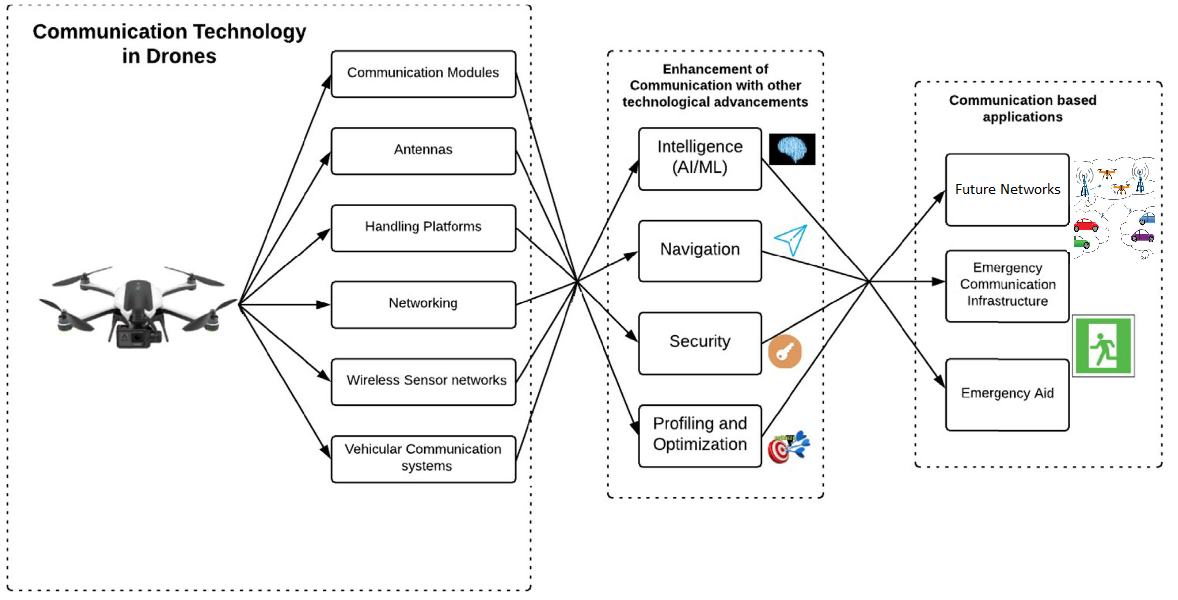
\includegraphics[width=1\linewidth]{figures/edited_scope_of_uav_communications.png}
    \caption{Applications \& Technologies of \acrshort{uav}s for Wireless Communication}
    \label{fig:scope_of_uav_comms}
\end{figure}
\acrshort{uav}s also can enhance the chance of dynamically establishing \acrfull{los} connections with a \acrfull{gu} in ways that are not possible with terrestrial and fixed network infrastructure.
\acrshort{uav}s can be designed and deployed to serve different roles in wireless communications networks, such as acting as a \acrfull{bs} or a relay. 

To ensure efficient use of \acrshort{uav}s as aerial \acrshort{bs}s is achieved, optimisation techniques and deep reinforcement learning (\acrshort{drl}) are employed to model the constraints on the system that are enforced upon an objective function. 
\acrshort{drl} is utilised to enable a \acrshort{uav} to adapt to a range of different scenarios rapidly. 

Simulations applying \acrshort{drl} to this joint optimisation problem have been created using the Python programming language  in which a set of legitimate ground users (\acrshort{gu}s), or legitimate users (\acrshort{lu}s), are provided with network coverage in a physically secure manner with the use of a \acrshort{uav}-\acrshort{bs} while a set of eavesdroppers (referred to as "Eves") who are attempting to conduct \acrfull{mitm} attacks are detecting the \acrshort{uav}-\acrshort{lu} signal that has been spiked with an \acrfull{ans}. 
\acrfull{bash} scripting has been used for running the experiments and handling the storage of the output data from the Python simulations for post-processing and analysis. 
The \acrshort{lu}s are able to filter out the \acrshort{ans}, whereas the Eve is not provided with the \acrshort{ans} information. 

Due to the large volume of data and the large number of highly non-linear relationships between many different aspects of the environment, quantum computing techniques are utilised to offload some of the computation that otherwise would be quite challenging to compute classically. 
This is also done to explore the concept of integrating contemporary quantum computing capabilities into a large and complex joint optimisation problem as this is a very new and developing field of study. 

This thesis aims to solve a joint optimisation problem for \acrshort{uav}-enabled wireless communications and networking with a particular focus on the physical layer security and secrecy of communications for a set of \acrshort{lu}s. 
To solve this joint optimisation problem, many different aspects of the system must be considered and the subproblems to the secrecy rate optimisation problem must also be optimised. 
To do this, the data exchange rate, energy efficiency and \acrshort{uav} trajectory are treated as subproblems to the secrecy rate optimisation problem and they are also optimised. 

As this is an exploration of future networking solutions, \acrfull{5g} and a \acrfull{mimo} system are considered for the wireless communications, with non-orthogonam multiple accessing (\acrshort{noma}) methods being used for the multiple-accessing required for the number of \acrshort{gu}s considered in the simulation environment. 
\chapter{Literature Review}

\section{Problem Area Contextualisation}
Due to advancements in the processing power of embedded systems and developments in small-scale, low-cost \acrshort{uav}s, the topic of multi-\acrshort{uav} enabled networks has become a focus of research with aims to practical implementations in recent years. Other relevant developments in networking include the development of communication schemes such as \acrlong{ofdm} (\acrshort{ofdm}), which is a spectrally efficient modulation scheme for \acrshort{4g} as well as \acrshort{noma} for \acrshort{5g} wireless communication standards. 

In regions where there is no network infrastructure, aerial alternatives that make use of \acrshort{uav}s, \acrlong{hap}s (\acrshort{hap}s) or both \acrshort{uav}s and \acrshort{hap}s can be utilised to serve the purpose of traditional network infrastructure. 
Such environments may include regions where there is no conventional network infrastructure due to the infrastructure being damaged or destroyed as a result of a natural disaster or where the region is too remote with terrain that is too inhospitable to feasibly construct the network infrastructure required for modern connectivity and security demands. This application is illustrated in Fig. \ref{fig:uav_public_safety}, which has been reproduced from \cite{saad_wireless_2020}. 

\begin{figure} [ht!]
    \centering
    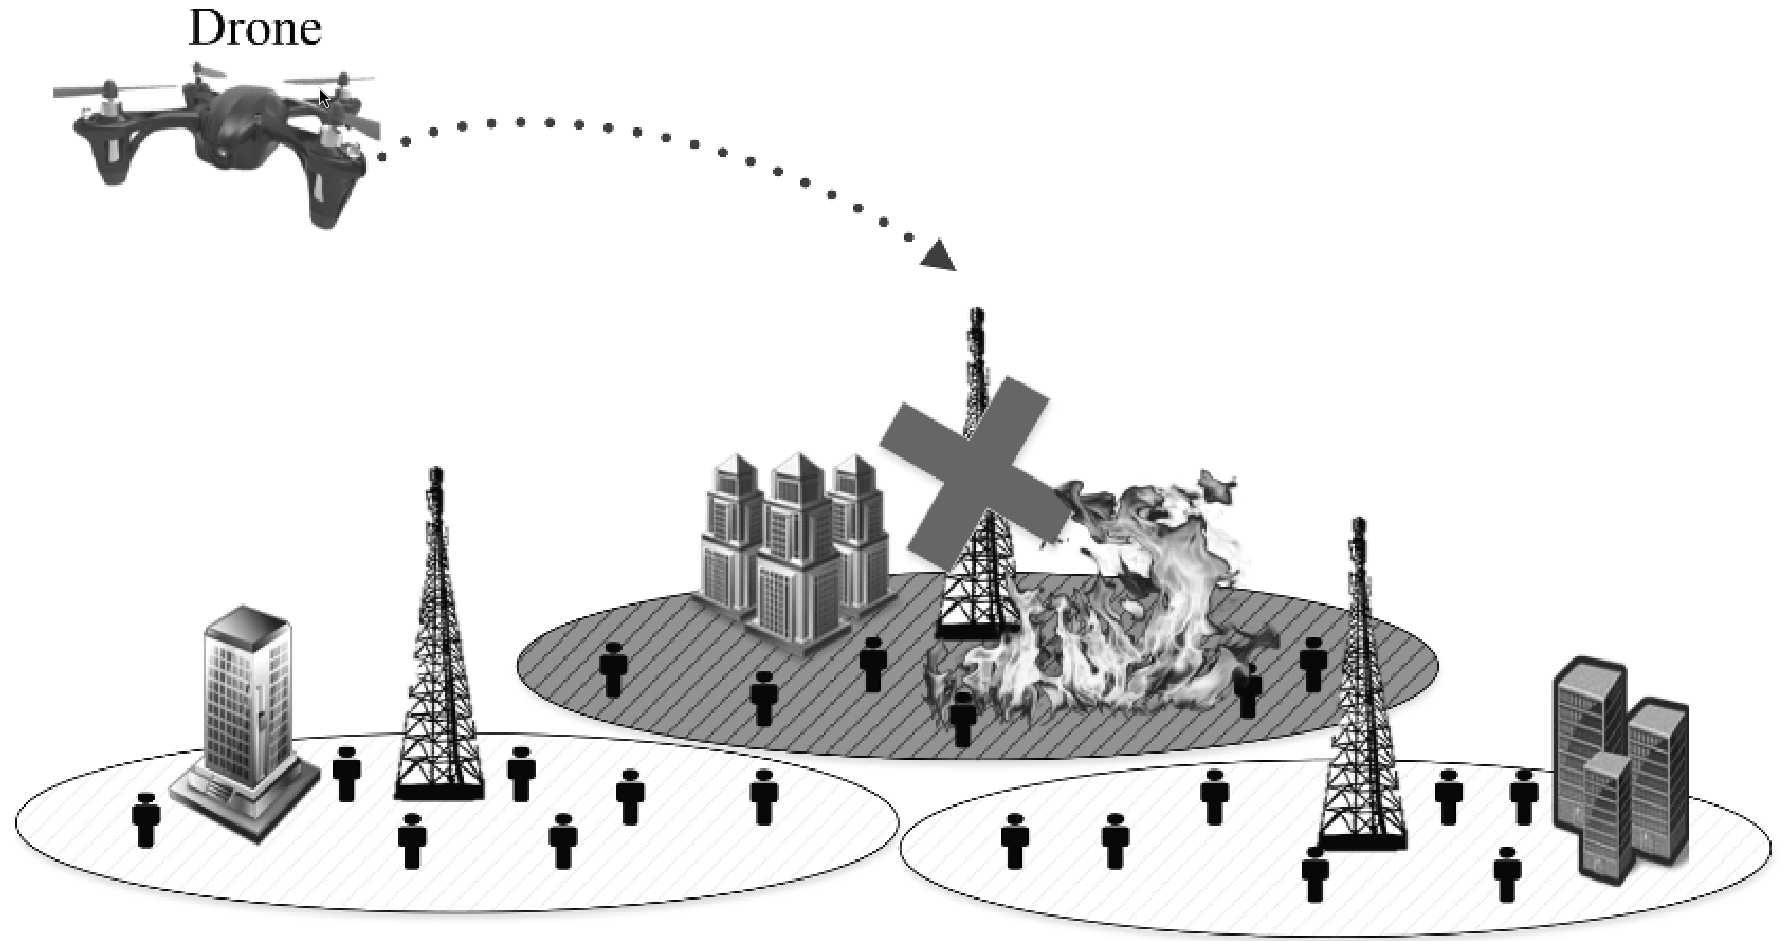
\includegraphics[width=0.75\textwidth]{figures/uav_public_safety_scenario.png}
    \caption{\acrshort{uav}s Acting as Network Infrastructure in a Disaster Scenario}
    \label{fig:uav_public_safety}
\end{figure}

Different approaches to this problem involving optimisation techniques will optimise a particular parameter as part of the system and treat others as constraints such that the best system performance with respect to the objective is achieved. 
This involves the design of algorithms based on closed-form mathematical derivations as well as numerical methods such as machine learning. 
Different system architectures are explored in the literature on this topic, which include \acrshort{uav}-\acrshort{hap}s aerial networks \cite{zhang_one_2025, ji_joint_2023, azizi_exploring_2024}, multi-\acrshort{uav} networks \cite{mu_security_2021, jeong_quantum_2025} and \acrshort{hap}-enabled networks. 

Optical communications exist and can be used effectively for secure wireless communications, however, the focus of this thesis and literature review is on radio communications as radio communications are more commonly used for wireless communications. 

Both quantum \cite{jeong_quantum_2025, silvirianti_layerwise_2024, li_intelligent_2021, saravanan_optimizing_2024} and classical optimisation techniques with applications to \acrshort{uav}-enabled networks have been explored in the literature. 

\section{Aerial Communications}
Airborne networks provide some benefits over terrestrial ones. One major benefit of airborne networks involving the use of \acrshort{uav}s for communications is that the networking platforms can reach higher altitudes than standard radio towers and their position can be adjusted dynamically to optimise their \acrfull{los} for air-to-air, air-to-ground and ground-to-air communications links. 
This is a substantial benefit over ground-based networks in regions where a clear \acrshort{los} cannot be attained easily, such as a dense urban environment, woodlands, etc., where communications links are otherwise very difficult to establish without the use of airborne communications platforms such as \acrshort{uav}s \cite{namuduri_uav_2017}.

\acrshort{uav}s can serve a variety of purposes as communications platforms. \acrshort{uav}s acting as a \acrfull{lap} oftentimes will have shorter missions and are more suitable for short-term, dynamic coverage, whereas \acrshort{hap}s are better utilised for longer-term missions \cite{namuduri_uav_2017}.

\acrshort{uav}s can serve a variety of purposes in an airborne communications network, such as acting as \acrshort{bs}s, relays, wireless \acrfull{ue} and others \cite{namuduri_uav_2017, saad_wireless_2020}.

\acrshort{uav}s can be used for jamming signals with a noise signature that is known by the friendly nodes in the network, such as \acrshort{gu}s, \acrshort{hap}s, \acrshort{bs}s, etc. and is unknown to eavesdroppers. These interfering signals can be used to mask the communication signals through a channel in a way that can be decoded by friendly actors in the network and serve as a challenge for eavesdroppers to be able to interpret the data being transmitted through an airborne network \cite{zhang_one_2025, lohan_secrecy-aware_2022}. 

%\subsection{\acrshort{uav}-\acrshort{hap}s Communications}
\subsection{\texorpdfstring{\acrshort{uav}-\acrshort{hap}s}{UAV-HAPs} Communications}
Both LAP and \acrshort{hap} \acrshort{uav}s can be used together \cite{zhang_energy-efficient_2024, ji_joint_2023, zhang_one_2025, qin_secure_2023} to create a network in which longer-term, more stable network coverage and communications are provided by the \acrshort{hap} portion of the system and the shorter-term, lower altitude communications are handled by the LAP portion of the system. 

Some challenges involving this kind of airborne network architecture involve the multiple degrees of freedom introduced by both \acrshort{hap} and LAP \acrshort{uav}s. This requires the use of optimisation algorithms being developed for various parameters involving both systems such that the entire system is performing as desired, i.e., with the most optimal outcomes depending on the focus of the network. 
Some examples of aspects of the system that require optimisation are the \acrshort{hap}/LAP deployment, energy efficiency of both \acrshort{hap}s and LAPs, resource allocation and secrecy \cite{zhang_one_2025}.
\begin{figure}[ht]
    \centering
    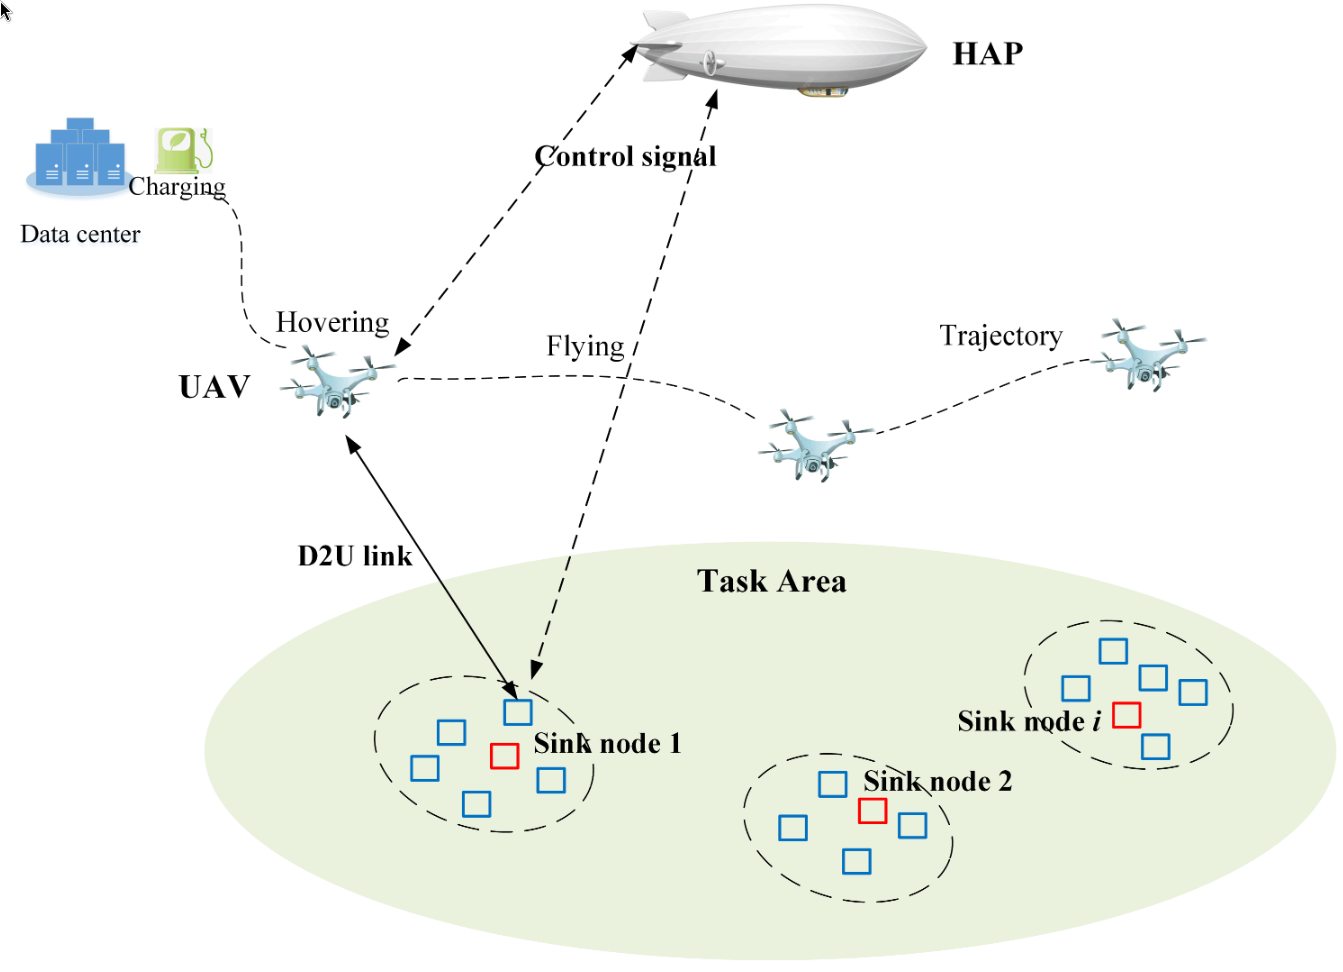
\includegraphics[width=0.75\textwidth]{figures/uav_hap_network_energy_efficient.png}
    \caption{Illustration of a \acrshort{uav}-\acrshort{hap} Network Model}
    \label{fig:energy_efficient_uav_hap_zhao}
\end{figure}
An illustration of a \acrshort{uav}-\acrshort{hap} network reproduced from \cite{zhao_energy_2023} is shown in Fig. \ref{fig:energy_efficient_uav_hap_zhao}, where \acrshort{uav}s and \acrshort{hap}s are integrated as an airborne network over a given task area to form device-to-\acrshort{uav} communications. These device-to-\acrshort{uav} communication links provide a means of communication between terrestrial terminal devices (\acrshort{td}s) or ground users (\acrshort{gu}s) in sink nodes. 

\subsection{\texorpdfstring{\acrshort{uav}s as Aerial \acrshort{bs}s}{UAVs as Aerial BSs}}
In the case of a \acrshort{uav} serving as an aerial \acrshort{bs}, the \acrshort{uav} itself is the provider of wireless communication services. For purposes such as this, the \acrshort{uav}s behave as low-altitude platforms (\acrshort{lap}s) and thus have a shorter mission time than \acrshort{hap}s or terrestrial \acrshort{bs}s. 

%Fig. \ref{fig:uav_aerial_bs_silvirianti} is taken from \cite{silvirianti_layerwise_2024} and depicts a wireless communications system in which \acrshort{uav}s act as aerial BSs in a network. 
%\begin{figure}[ht]
%    \centering
%    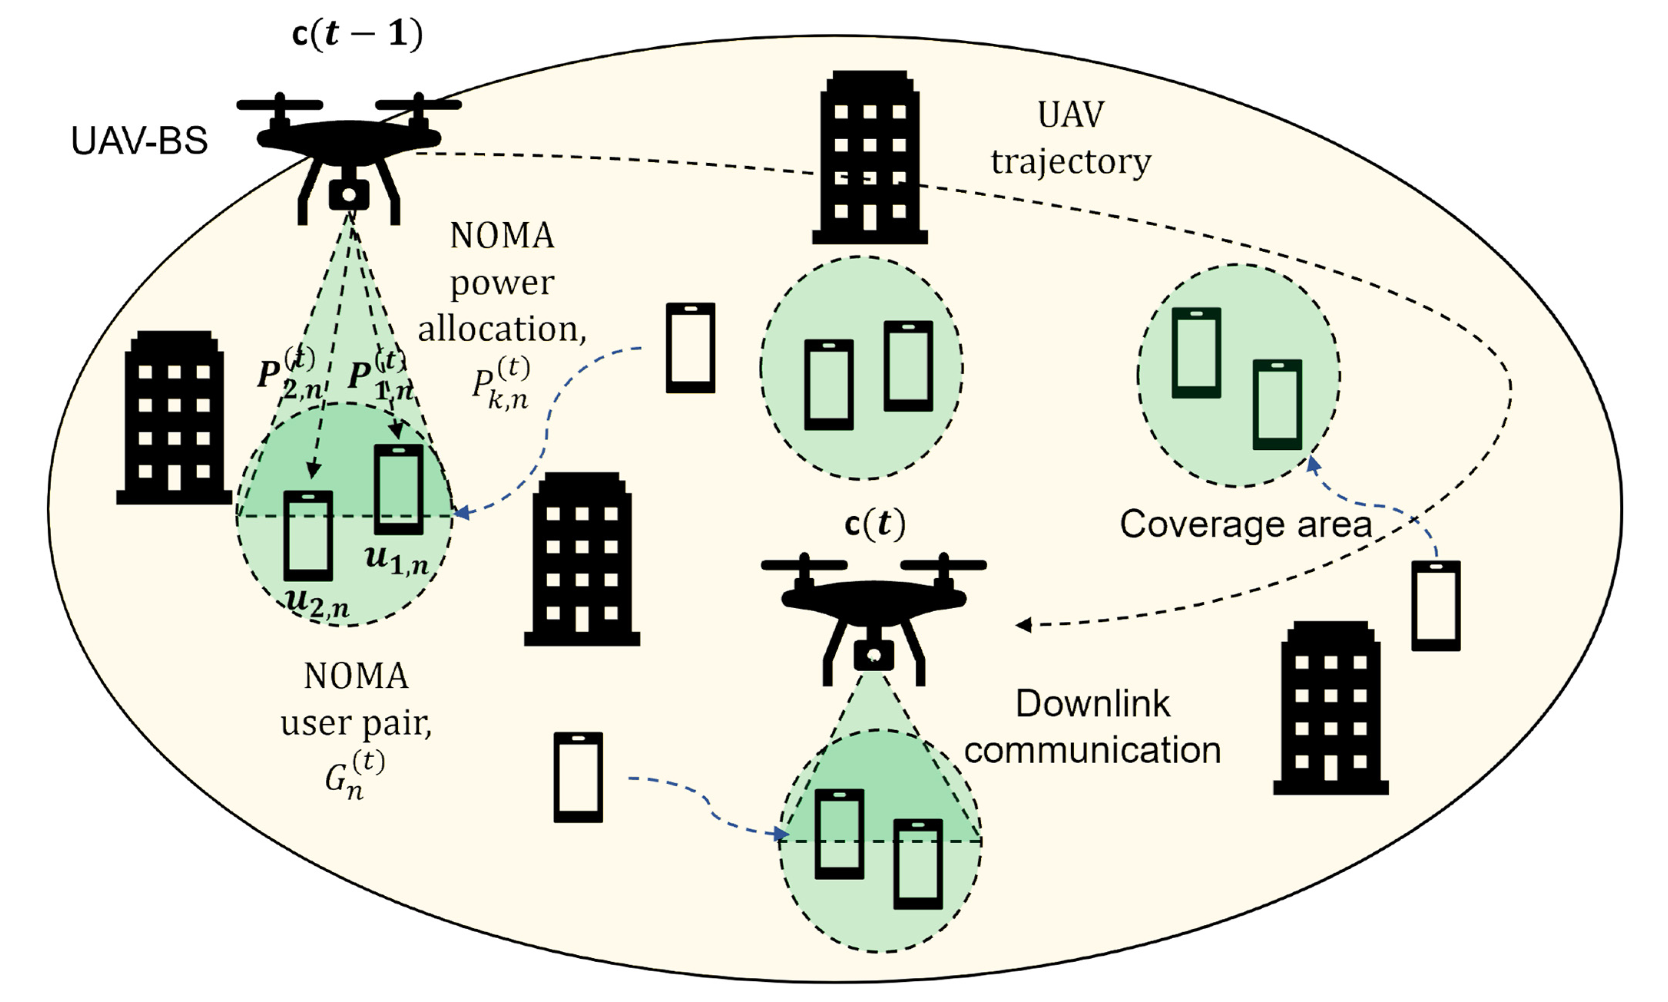
\includegraphics[width=0.75\textwidth]{figures/uav_as_aerial_bs_silviratani_et_al.png}
%    \caption{Network in which \acrshort{uav}s act as Aerial BSs to Provide Coverage to \acrshort{gu}s}
%    \label{fig:uav_aerial_bs_silvirianti}
%\end{figure}
For network architectures like this, the deployment will constantly be changing and thus, typically requires some optimisation of the \acrshort{uav} deployment. 
This constantly changing positioning and deployment model also introduces a need for a channel model that can accurately describe this form of \acrshort{bs} \cite{saad_wireless_2020}. 

\subsection{\texorpdfstring{\acrshort{uav}s}{UAVs} as Relays}
\acrshort{uav}s can be used to extend the range of coverage for a terrestrial or airborne network by serving as network relays between \acrshort{bs}s \cite{zhang_energy-efficient_2024, namuduri_uav_2017, saad_wireless_2020}. 

Fig. \ref{fig:uav_as_relay_namuduri} is a diagram reproduced from \cite{namuduri_mobile_nodate} depicting a \acrshort{uav} serving as a relay between two terrestrial \acrshort{bs}s. 
\begin{figure}[ht]
    \centering
    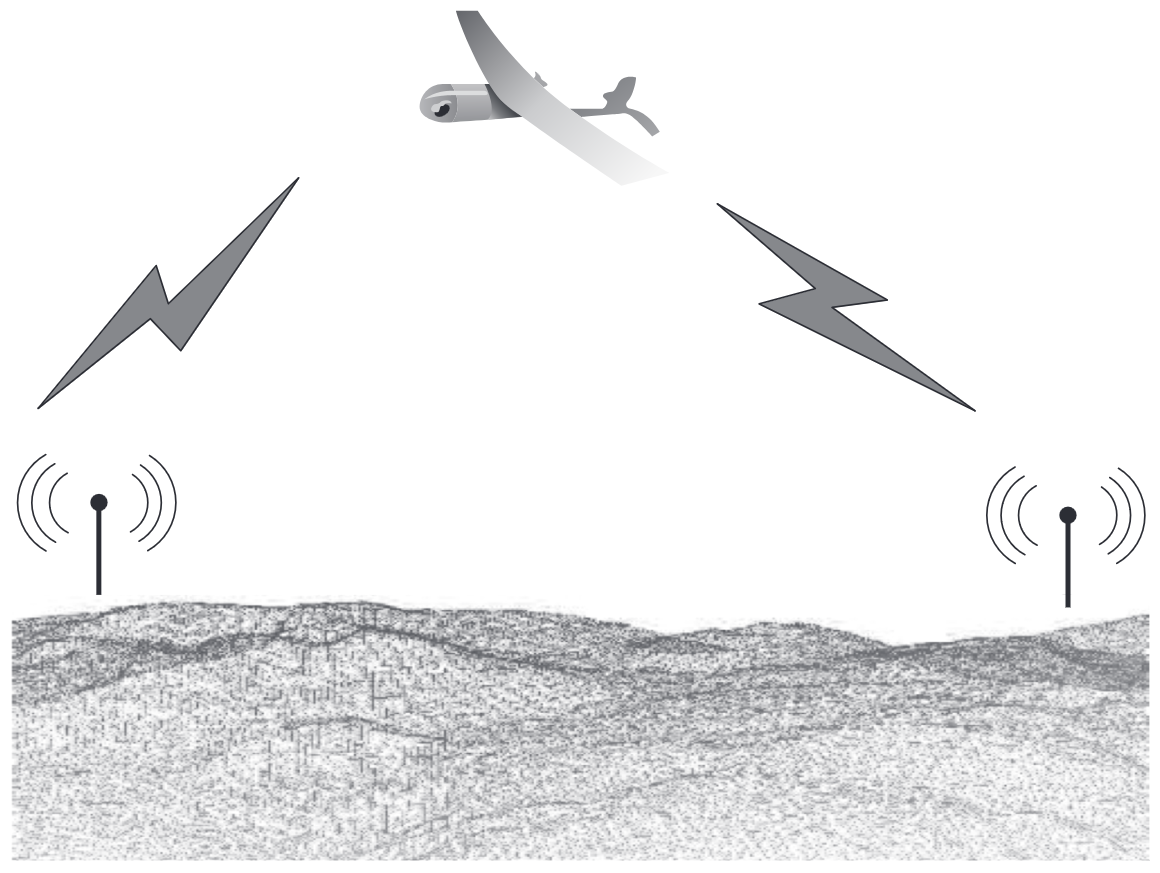
\includegraphics[width=0.75\textwidth]{figures/uav_as_relay_saad_textbook.png}
    \caption{\acrshort{uav} Acting as a Relay Between 2 \acrshort{bs}s}
    \label{fig:uav_as_relay_namuduri}
\end{figure}
\acrshort{uav}s acting as relays for a network can be used to overcome challenges involving poor LoS between other links in a network due to their ability to overcome environmental obstacles dynamically in ways that terrestrial \acrshort{bs}s cannot. 

The use of \acrshort{uav}s as relays does present its own set of challenges, however. Some of these include the necessity to adapt existing relaying mechanisms or to devise novel relaying schemes. 
To ensure proper relaying is achieved, the information related to the control systems of the \acrshort{uav}s, such as their position, altitude, environmental conditions, available resources, etc. must be communicated and known by other \acrshort{uav}s that are directly communicating with it within the network \cite{saad_wireless_2020}. 
Air-to-air links in particular have changing propagation environments, which will be changing frequently as the \acrshort{uav} relays are adjusting their positions and altitude as part of any given mission. 
Multi-hop \acrshort{uav} relays for air-to-air links require the use of dynamic routing algorithms based on the control and communications data from the \acrshort{uav}s in the network, which can be quite challenging to implement on small-scale embedded systems frequently used in small-scale \acrshort{uav}s \cite{saad_wireless_2020}. 

%\subsection{\acrshort{uav}s as \acrshort{ue}s}
\subsection{\texorpdfstring{\acrshort{uav}s as \acrshort{ue}s}{UAVs as UEs}}
\acrshort{uav}s may act as user equipment (\acrshort{ue}) to communicate with existing wireless communication networks, such as WiFi or cellular networks. 
A key challenge involving \acrshort{uav}s as wireless \acrshort{ue}s is that existing terrestrial \acrshort{bs}s have been optimised and designed to provide the best coverage to \acrshort{gu}s rather than airborne \acrshort{ue}s. This has been achieved by designing the main antennae lobes on such \acrshort{bs}s such that they're pointing downwards towards \acrshort{gu}s \cite{saad_wireless_2020}. 
Furthermore, \acrshort{gu}s and \acrshort{uav} \acrshort{ue}s must be differentiated by the network operators to distinguish both classes of user, which has not been a commonly implemented mechanism in conventional networking technologies for \acrshort{ue}s. 

Some applications of cellular-connected \acrshort{uav}-\acrshort{ue}s are presented in Fig. \ref{fig:uav_ue_applications}, which has been adapted from \cite{challita_machine_2019}. 

\begin{figure}[ht!]
   \centering
       \subfigure[\acrshort{uav}-\acrshort{ue}s used in Intelligent Transport Systems]{\label{uav_ue_transport_challita}
           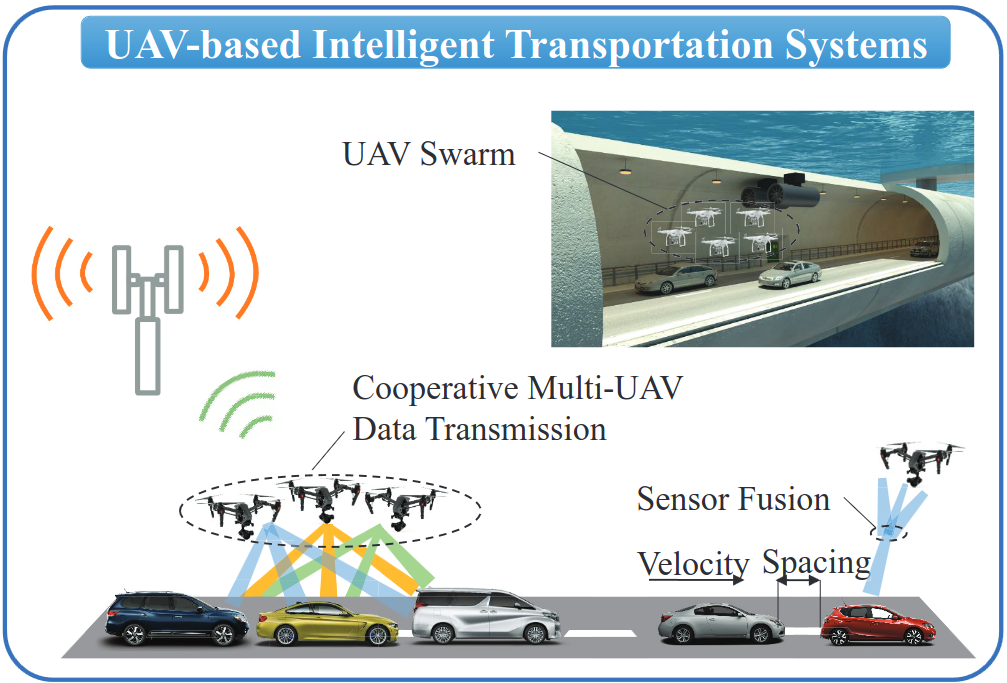
\includegraphics[height=0.2\textheight]{figures/uav_ue_transportation.png}
       }
       \hspace{1mm}
    \subfigure[\acrshort{uav}-\acrshort{ue}s used in Delivery Systems]{\label{uav_ue_delivery_challita}
           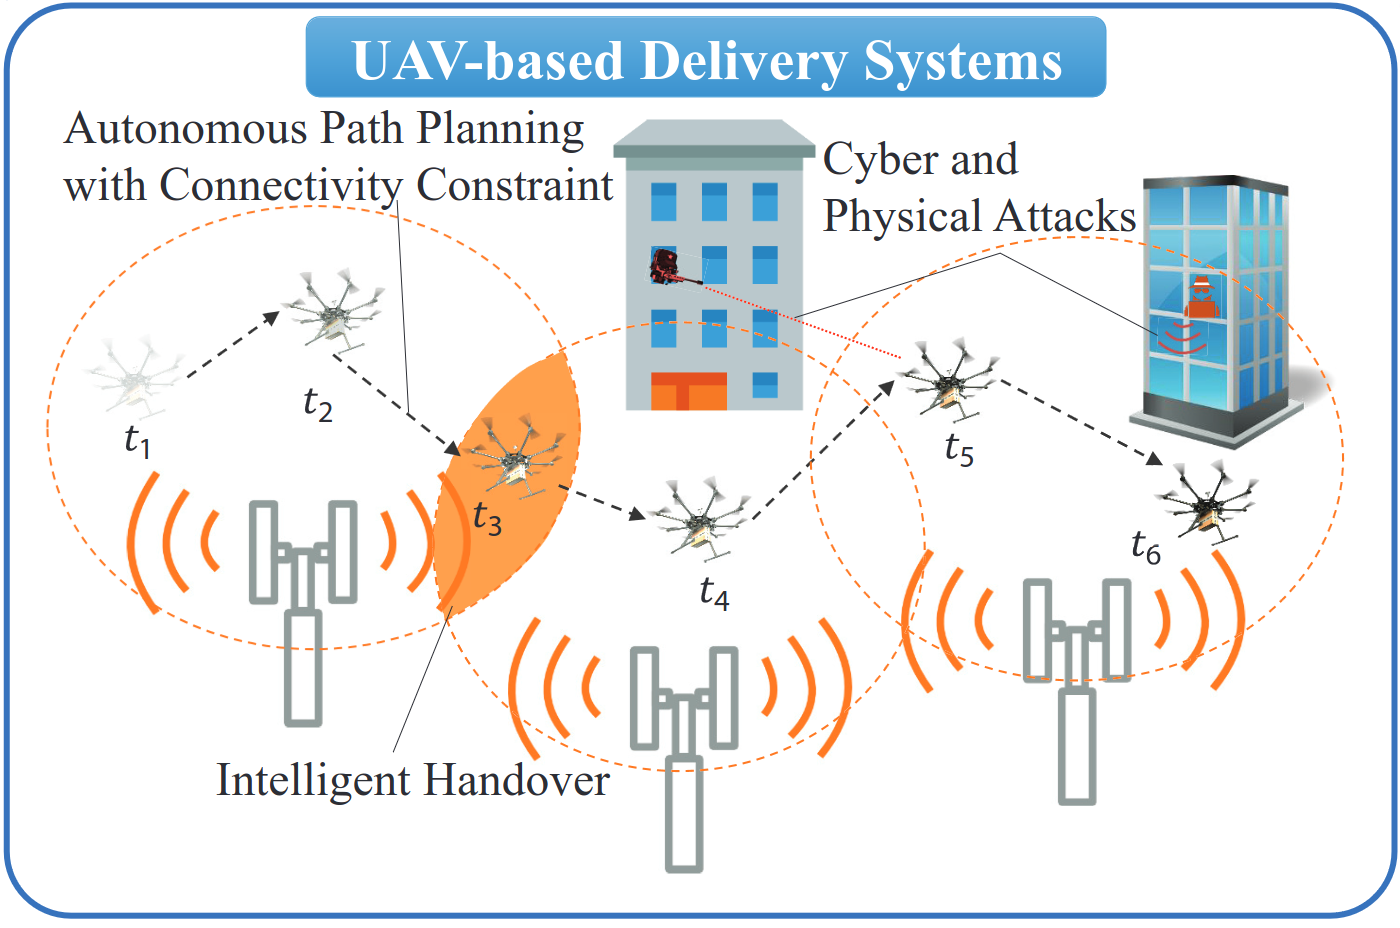
\includegraphics[height=0.2\textheight]{figures/uav_ue_delivery.png}
       }
       \hspace{1mm}
    \subfigure[\acrshort{uav}-\acrshort{ue}s used for Multimedia Streaming]{\label{uav_ue_multimedia_challita}
            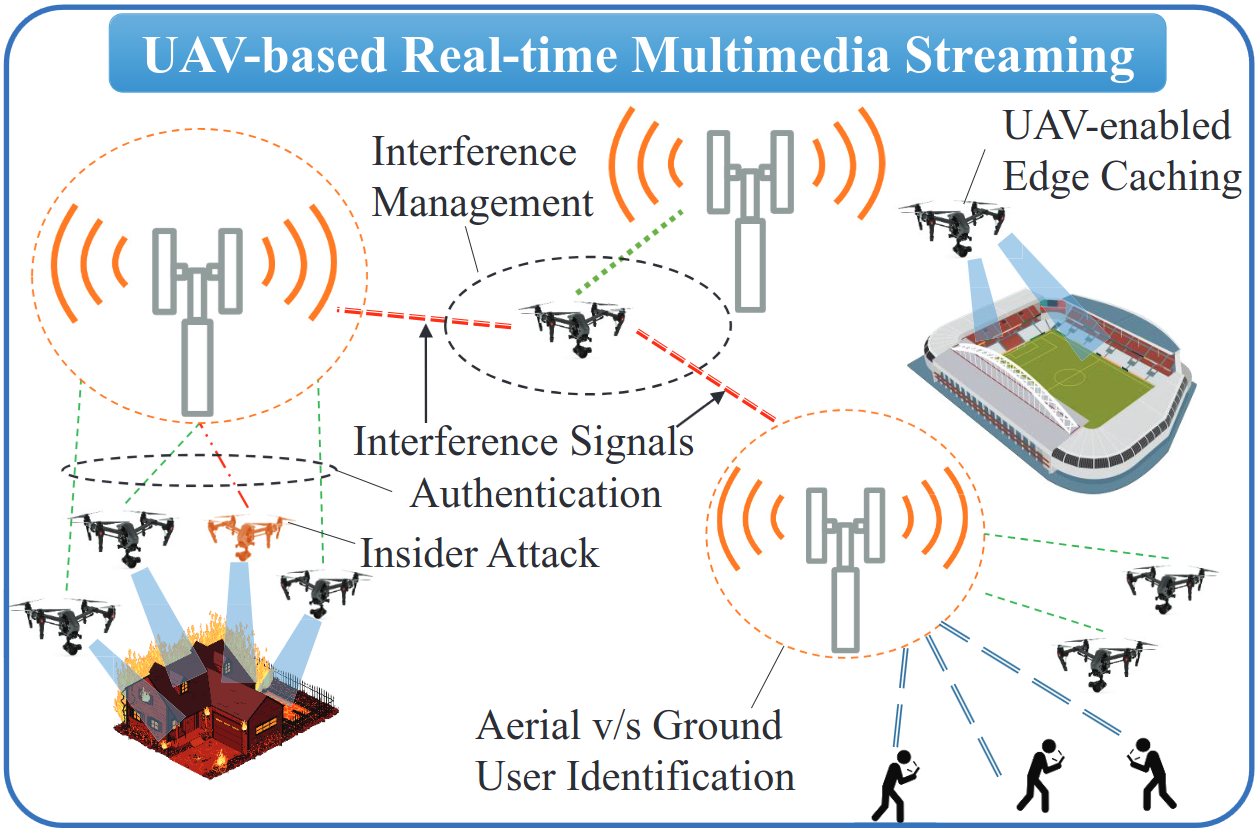
\includegraphics[height=0.2\textheight]{figures/uav_ue_multimedia.png}
        }
       \caption{\acrshort{uav}-\acrshort{ue}s used in Various Systems}
       \label{fig:uav_ue_applications}
\end{figure} 
Cellular-connected \acrshort{uav}s provide beyond \acrshort{los} control, low latency, real-time communication, wide levels of coverage and robust security \cite{challita_machine_2019}, which is advantaged over \acrshort{uav} \acrshort{ue}s connected to a network over short-range communication schemes such as WiFi or Bluetooth. 

\subsection{\texorpdfstring{Ad-Hoc \acrshort{uav}}{Ad-Hoc UAV} Networks}
Mobile ad hoc networks (\acrshort{manet}s) are self-organising networks that are formed by mobile nodes \cite{namuduri_mobile_nodate, namuduri_uav_2017, sahingoz_mobile_2013}. This literature review focuses particularly on \acrshort{uav}-enabled \acrshort{manet}s, however, other forms of \acrshort{manet} can exist, such as ground vehicle-enabled \acrshort{manet}s \cite{namuduri_mobile_nodate}. 

\acrshort{uav}-enabled \acrshort{manet}s are multi-hoop networks that can be used for transmitting and receiving information over long distances. 
Fig. \ref{fig:uav_ad_hoc_namuduri} depicts an ad-hoc configuration of a \acrshort{uav}-based network architecture reproduced from \cite{namuduri_mobile_nodate}. 

\begin{figure}[ht]
    \centering
    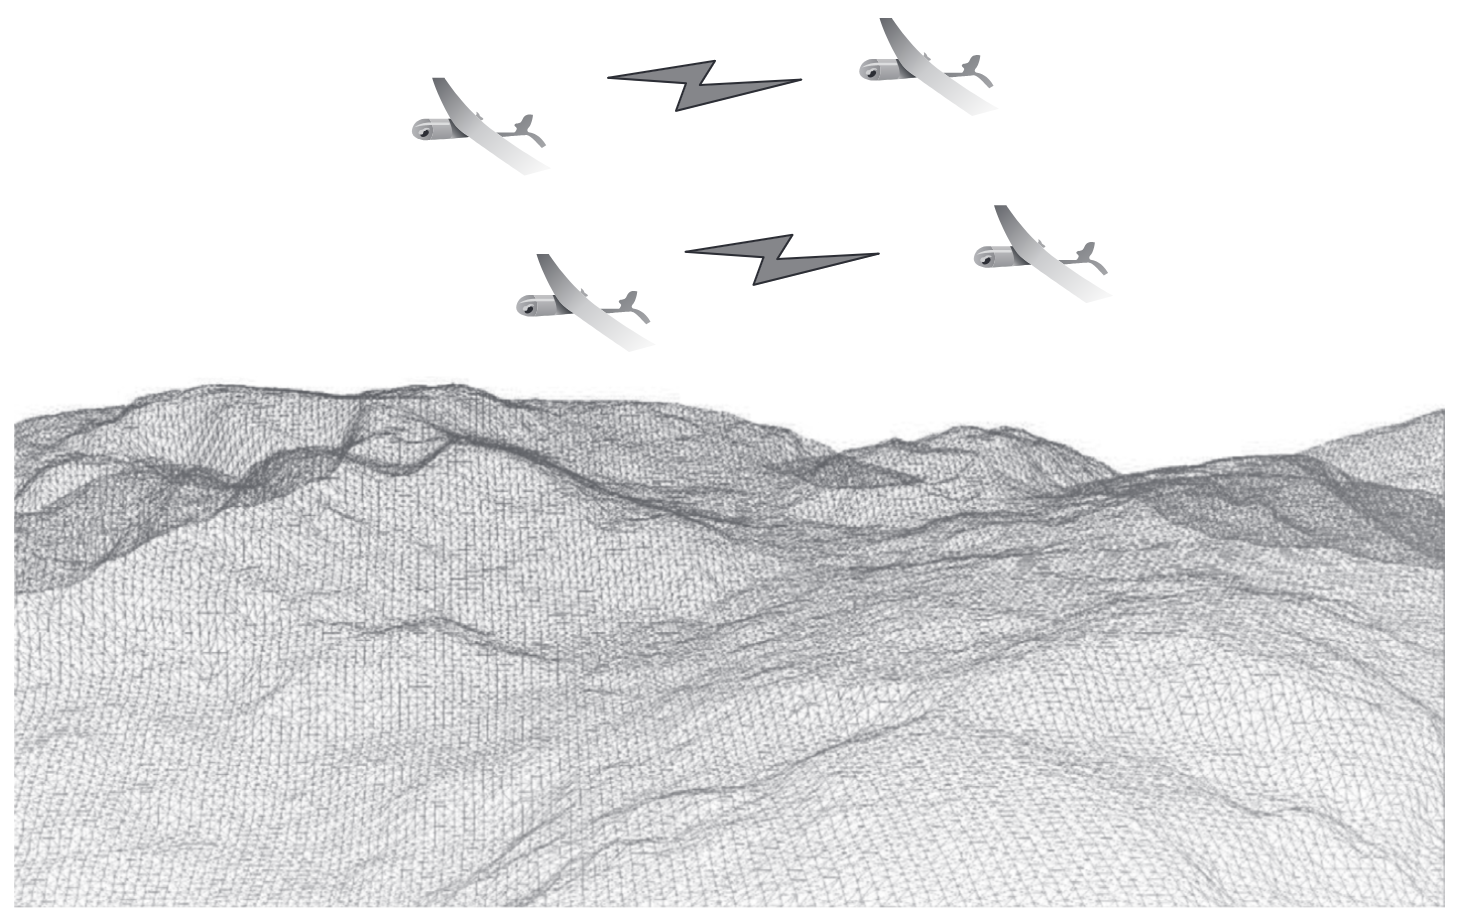
\includegraphics[width=0.75\textwidth]{figures/uav_ad_hoc_saad_textbook.png}
    \caption{Ad Hoc Configuration of \acrshort{uav} Network}
    \label{fig:uav_ad_hoc_namuduri}
\end{figure}
\acrshort{manet}s do not require the use of other network infrastructure, such as satellites or centralised servers to support the swarm of vehicles \cite{namuduri_uav_2017}, however, it's also expected that there is some assistance from terrestrial control stations as part of the network architecture \cite{namuduri_mobile_nodate}. 
Each node in the \acrshort{uav}-enabled \acrshort{manet} acts as a relay, router and terminal. 

\section{Optimisation of \texorpdfstring{\acrshort{uav}}{UAV} Communications}
%\hl{Write about what system parameters have been optimised to date in the literature, i.e., the objective and what the constraints are on that objective here}
%\\
%\hl{Compare different approaches to the problem and the key parameters that are and aren't important for different problems, e.g., energy efficiency/power consumption is a universal problem but secrecy may not be for some applications}.
%\\
%\hl{Refer to the papers saved in Zotero covering classical optimisation techniques used for systems/problems like this}
%\\
For optimal performance of an airborne network, optimisation techniques have been employed with a range of focuses for optimisation and constraints of a given system. 
The objective functions are typically mathematically derived and proven in the literature and algorithms are designed to implement them for the communications and control systems involved in airborne networks. 

Different studies focus on various aspects of airborne networks, with emphases placed on particular objectives of the system subject to a variety of relevant constraints. 
Many of these studies are presented with a joint non-convex optimisation problem that cannot be solved efficiently or easily with a standalone algorithm and thus, piecewise approaches are taken to optimise particular parameters of the system individually without violating the constraints of the overall problem. 
The main factors for optimisation that have been explored in the literature on this topic include energy efficiency \cite{zhao_energy_2023, zhang_energy-efficient_2024}, \acrshort{uav} clustering \cite{zhao_energy_2023, jeong_quantum_2025}, communication secrecy \cite{zhang_one_2025, mu_security_2021, yan_secure_2022}, platform deployment \cite{ji_joint_2023}, \acrshort{uav} trajectory \cite{zhao_energy_2023}, latency \cite{saravanan_optimizing_2024}, resource allocation\cite{ji_joint_2023} and scheduling, to name a few. 

The following subsections detail a set of focal points for optimisation and the constraints that are considered for aerial communications that have been documented to date. 
\subsection{Security \& Secrecy}
A key focus of many of these studies is the secrecy of communication and ensuring that the communications are secure between \acrshort{gu}s, \acrshort{hap}s and LAPs\cite{qin_secure_2023, zhang_one_2025, yan_secure_2022, mu_security_2021, lohan_secrecy-aware_2022}. In \cite{zhang_one_2025}, \acrshort{hap}s are deployed for communication with \acrshort{gu}s and \acrshort{uav}s are used for detection of eavesdroppers, who are referred to as "Eves" in the paper. 

\begin{figure}[ht!]
    \centering
    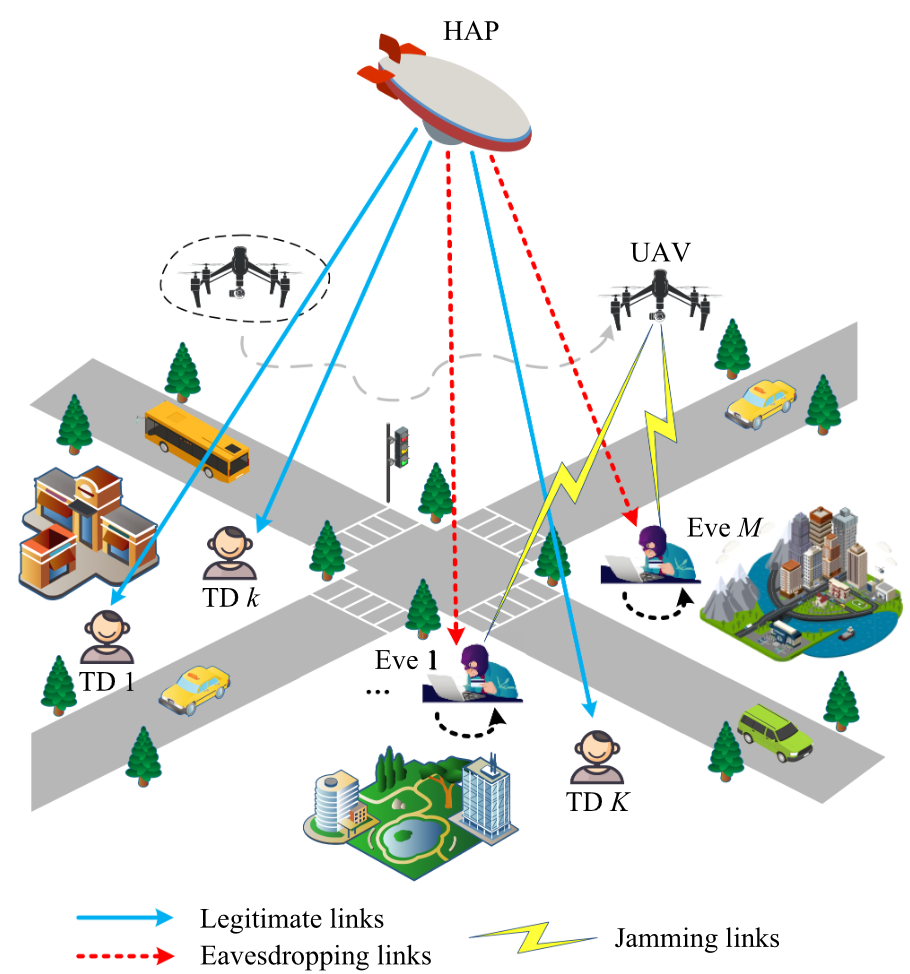
\includegraphics[width=0.7\textwidth]{figures/uav_haps_eves_diagram.png}
    \caption{Illustration of a Secure \acrshort{uav}-\acrshort{hap} Network Model}
    \label{fig:secure_uav_hap_zhang}
\end{figure}
An illustration of a secure \acrshort{uav}-\acrshort{hap} network reproduced from \cite{zhang_one_2025} is shown in Fig. \ref{fig:secure_uav_hap_zhang}, where \acrshort{uav}s are used as jammers to combat eavesdroppers and the \acrshort{hap} is used as the network provider for communication links between terrestrial \acrshort{td}s. 
The \acrshort{hap} network uses a \acrshort{uav} to interfere with the signal decoding of multiple mobile eavesdroppers. 
The \acrshort{uav}'s trajectory is dynamically adjusted and optimised based on the known locations of the eavesdroppers. 

In this study, the system's orthogonal subcarrier scheduling among \acrshort{td}s, subcarrier power allocation, \acrshort{uav} trajectory and \acrshort{hap} deployment are jointly optimised to maximise the minimum average secrecy rate (\acrshort{masr}), subject to the constraints of \acrshort{uav} mobility and \acrshort{hap} power budget.
This optimisation problem is a mixed-integer, non-convex optimisation problem, however, it is solved iteratively using successive convex approximation (\acrshort{sca}) algorithm. This is achieved by alternately optimising the \acrshort{uav} trajectory, power allocation and the subcarrier scheduling until convergence. 

Another approach to ensuring secrecy of communication is detailed in \cite{qin_secure_2023}, where the secrecy considerations are modelled as constraints in the system rather than objectives and the task computation latency, task scheduling and transmit power of legitimate users (\acrshort{lu}s) are jointly optimised for secure mobile edge computing (\acrshort{mec}). The system model is shown in Fig. \ref{fig:qin_uav_hap_mec_system_model}, which has been reproduced from \cite{qin_secure_2023}.

\begin{figure}[ht!]
    \centering
    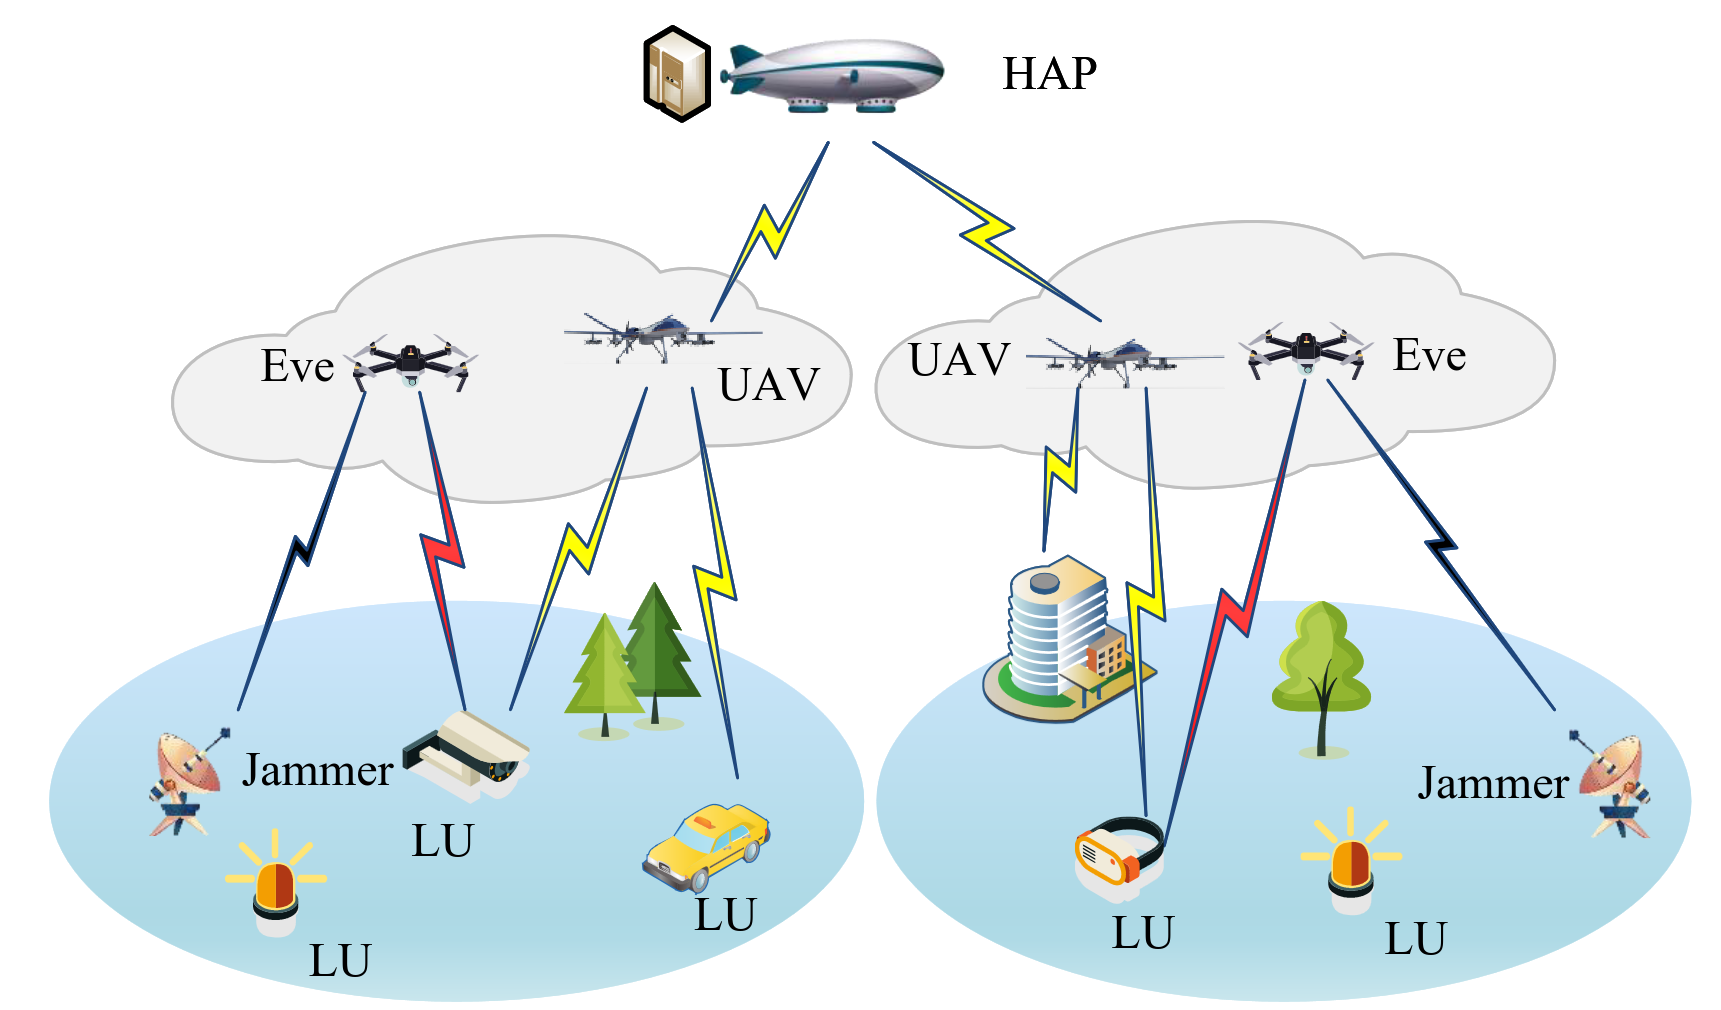
\includegraphics[width=0.75\textwidth]{figures/uav_hap_secrecy_qin.png}
    \caption{\acrshort{uav}-\acrshort{hap}-Enabled System Model for Secure \acrshort{mec}}
    \label{fig:qin_uav_hap_mec_system_model}
\end{figure}

An iterative approach is also taken for this proposed form of optimisation as in the case of \cite{zhang_one_2025}, in which the joint non-convex optimisation problem is solved by individually optimising the various parameters such that the minimum secure offloading sum rate is maximised. 
\acrshort{noma} is utilised for spectral efficiency over \acrshort{ofdm} as it allows multiple users to transmit data over the same resource block, so it supports a greater level of spectral efficiency \cite{qin_secure_2023}. 

\subsection{Energy Efficiency}
Certain studies \cite{silvirianti_energy-efficient_2022, silvirianti_layerwise_2024, zhao_energy_2023, zhang_energy-efficient_2024} focus on maximising the energy efficiency of \acrshort{uav}s in airborne networks. The importance of optimising the energy efficiency of the airborne platforms can be viewed as a universal one for the optimisation of any given \acrshort{uav} mission for networking due to the limited power capacity of LAPs, in particular that typically cannot generate any power while they're operational. 

In \cite{zhao_energy_2023}, the trajectory of \acrshort{uav}s in the network is optimised jointly with the resource allocation for the \acrshort{uav}s to maximise the energy efficiency. 
A dynamic, self-adaptive clustering algorithm based on affinity propagation and a proximal policy optimisation (\acrshort{ppo}) based deep reinforcement learning (\acrshort{drl}) algorithm are used to optimise the \acrshort{uav} clustering, trajectory planning and transmit power level of the sensing devices for providing device-to-\acrshort{uav} communication. 
In this study, \acrshort{hap}s are used as aerial \acrshort{bs}s, whereas the \acrshort{uav}s are used for the device links and communication with the \acrshort{hap}s that are providing the networking coverage. 
The simulation of the algorithm uses a scenario involving network that consists of a single \acrshort{uav} and \acrshort{hap}-\acrshort{bs} using the clustering and resource allocation algorithms to maximise the energy efficiency. 

The approach taken in \cite{zhang_energy-efficient_2024} involves the optimisation of the energy efficiency using the transmission power, \acrshort{uav} altitude and time allocation of \acrshort{hap}s and \acrshort{uav}s in the network. The architecture considered is a two-hop \acrshort{hap}-\acrshort{uav}-assisted wireless network that is serving a set of \acrshort{gu}s. 

The energy efficiency is maximised such that it does not violate the constraints of \acrshort{uav} altitude, \acrshort{uav} and \acrshort{hap} transmit power and the total operation time. 

Three algorithms are utilised to meet this objective, algorithm 1 handles the global optimal \acrshort{uav} and \acrshort{hap} transmit power, algorithm 2 handles the optimal transmit power allocation for the \acrshort{uav}s and \acrshort{hap}s alternately and algorithm 3 directly handles the energy efficiency using the optimal transmit power and allocation for the \acrshort{uav}s and \acrshort{hap}s, thus algorithm's 3 complexity and efficacy is dependent on the performance and adoption of algorithms 1 and 2 \cite{zhang_energy-efficient_2024}.

\subsection{Resource Allocation}
The allocation of resources within the network is a focus for optimisation in airborne networks. In \cite{ji_joint_2023}, a joint resource allocation problem is formulated and divided into constituent subproblems. The iterative algorithm proposed in \cite{ji_joint_2023} is sub-optimal, however, it can solve the resource allocation and \acrshort{hap} deployment optimisation problems efficiently and separately.

The resource allocation algorithm is based on the Gale-Shapely algorithm to produce a convergent solution to the two-sided matching game of the \acrshort{hap} deployment and resource allocation algorithms. 
Both algorithms are combined into a single algorithm that alternates between solving each of these problems iteratively, thus reducing it from a joint optimisation problem to two smaller subproblems for the algorithm to solve more efficiently. 

\section{Quantum Computing Techniques}
In recent years, quantum computers have been developed in an attempt to compute problems that cannot be solved as effectively, or at all, using classical computers. Different approaches to create qubits that leverage different technologies such as ion trap qubits \cite{Bruzewicz_2019}, superconducting qubits \cite{Krantz_2019}, semiconductor qubits \cite{chatterjee_semiconductor_2021} and photonic qubits \cite{Kok_2007}. 

Hybrid classical-quantum computer implementations have also been explored as feasible solutions to solving optimisation problems where some of the computation can be offloaded to one or the other means of computation depending on which method is more suitable to a portion of any given problem. 

Quantum computing can be utilised to solve complex optimisation problems. 

The two leading quantum computing paradigms are gate-based quantum computing and \acrfull{aqc} \cite{yarkoni_quantum_2022}. Gate-based quantum computing involves the application of a sequence of unitary quantum gates to a set of qubits. The states of the qubits collapse into a $\ket{0}$ or $\ket{1}$ state upon measurement. 

\acrshort{aqc} involves the preparation of a multi-qubit state as the ground state of a Hamiltonian operator. This Hamiltonian then has an adiabatic time evolution applied to it, which changes the Hamiltonian such that its ground state encodes the solution of the optimisation problem \cite{yarkoni_quantum_2022}. 
\subsection{Quantum Annealing}
Quantum annealing is a heuristic optimisation algorithm that can be used to solve combinatorial optimisation problems \cite{yarkoni_quantum_2022}.
With the use of quantum annealing, an optimisation problem can be converted into \acrlong{qubo} (\acrshort{qubo}) or Ising models \cite{jeong_quantum_2025}.
The expression for the \acrshort{qubo} problem is shown in \ref{eq:qubo}.
\begin{equation} \label{eq:qubo}
        Obj(x, Q) = x^T \cdot Q \cdot x
\end{equation}
Where $x$ is the vector of $N$ binary variables and $Q$ is the symmetric matrix defining interaction terms between the variables, which is an upper diagonal matrix  \cite{jeong_quantum_2025, yarkoni_quantum_2022}. 
In the case of the \acrshort{qubo} in \cite{jeong_quantum_2025}, the goal is to minimise $x$ in the objective function, so the \acrshort{qubo} is expressed as shown in \ref{eq:min_qubo}.
\begin{equation} \label{eq:min_qubo}
    \underset{x}{\min}\ H_{\acrshort{qubo}}(x) = x^{T} \cdot Q \cdot x
\end{equation}
The \acrshort{qubo} model can be extended to represent the binary combinatorial optimisation problem with linear and quadratic terms and, in this case, an $N \times N$ binary vector in 2 dimensions is considered. This model can be expressed as \ref{eq:lin_quad_qubo}. 
\begin{equation} \label{eq:lin_quad_qubo}
    H_{\acrshort{qubo}}(x) = \sum_{i=1}^{N} Q_{ii}x_{i} + \sum_{i=1}^{N}\sum_{j=1}^{N} Q_{ij} x_{i} x_{j}
\end{equation} 
In \cite{jeong_quantum_2025}, two quantum annealing-based algorithms are used for the optimisation of \acrshort{uav} clustering and for sub-channel assignment and power allocation. This algorithm is described pictorially in Fig. \ref{fig:quantum_annealing_uav_jeong}, which has been reproduced from \cite{jeong_quantum_2025}. 

\begin{figure}[ht]
    \centering
    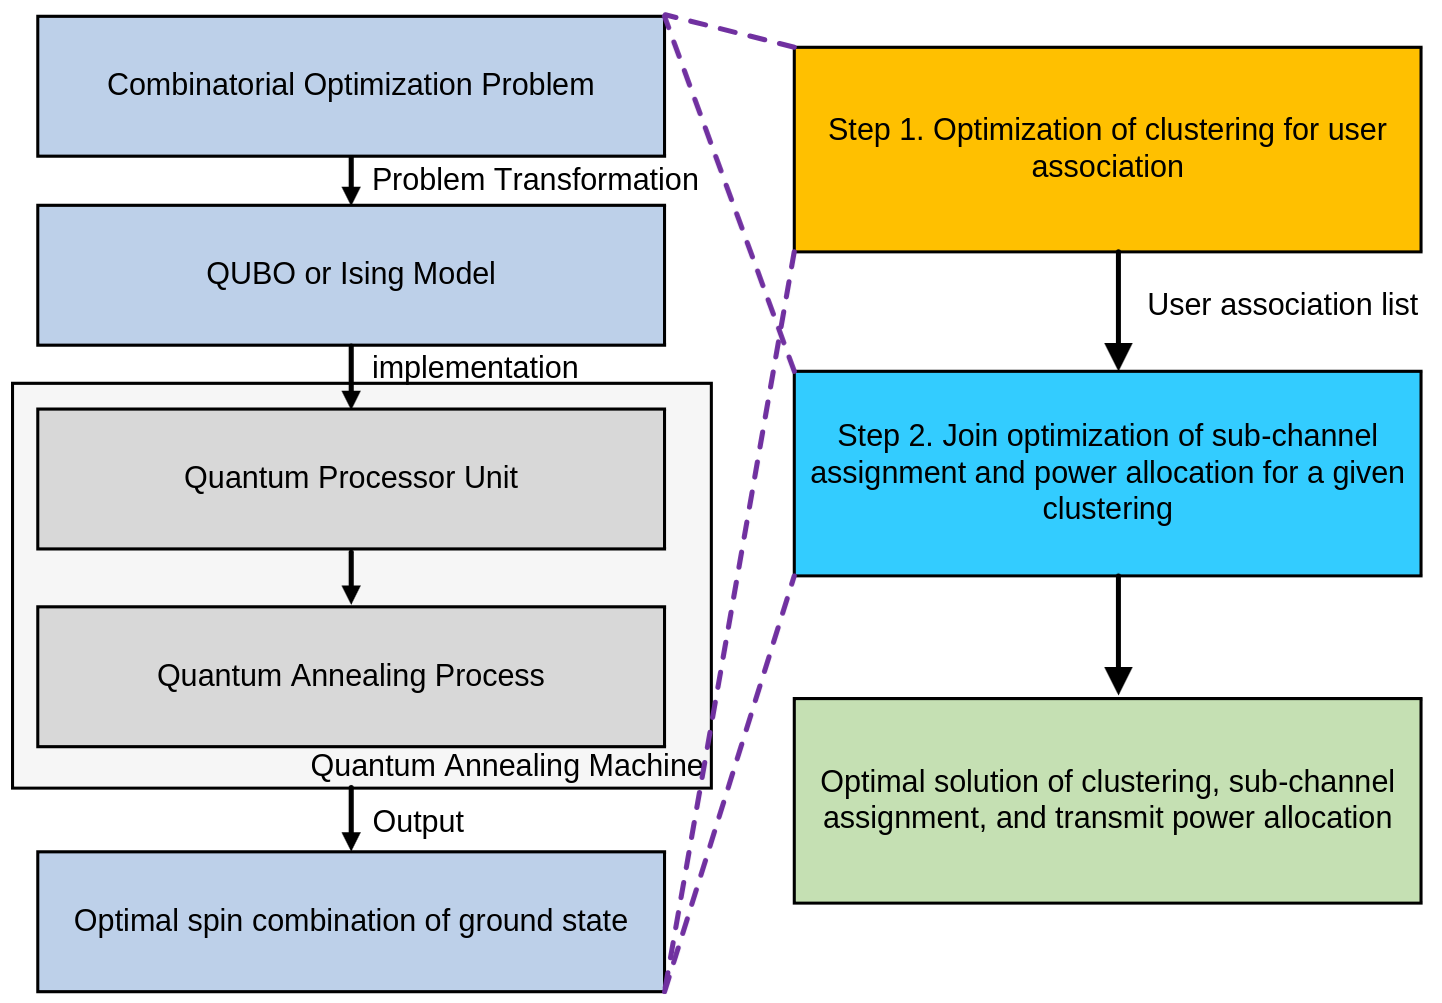
\includegraphics[width=1\textwidth]{figures/quantum_annealing_uav_algorithm.png}
    \caption{Quantum Annealing Based Algorithms for Optimisation of Clustering, Sub-Channel Assignment and Power Allocation}
    \label{fig:quantum_annealing_uav_jeong}
\end{figure}
In \cite{jeong_quantum_2025}, a quantum annealing-based clustering algorithm with a constrained quadratic model (\acrshort{cqm}) is used to optimise a binary variable that indicates if a \acrshort{uav} is associated with a \acrshort{gu} or not. 
The algorithm takes the locations of the \acrshort{gu}s and \acrshort{uav}s and builds the \acrshort{cqm} object. It then maps the cost function for optimising the \acrshort{uav} and \acrshort{gu} clustering to a \acrshort{qubo} Hamiltonian that is energy-based for use with D-Wave's quantum annealing machine, runs the \acrshort{cqm} sampler and then returns the optimal spin combination for the association of \acrshort{gu}s with \acrshort{uav}s for clustering. 
This algorithms provides the clustering configuration for the \acrshort{uav}s for the set of \acrshort{gu}s. 
The next algorithm handles the joint optimisation of the power allocation and sub-channel assignment for this clustering configuration that has been determined. 

The proposed quantum annealing based algorithm using a D-Wave hybrid \acrshort{qubo} solver outperformed classical K-means, simulated annealing \cite{kirkpatrick_optimization_nodate} and steepest descent \cite{battiti_first-_1992} algorithms in terms of maximisation of the sum rate, measured in Mbps. 
This increase in the quantum annealing based algorithms' performance also scaled better than the pre-existing algorithms with increases in the number of \acrshort{gu}s. 
The simulation time was also faster and remained low for increasing numbers of \acrshort{uav}s where the simulation time of the other algorithms began to increase for increasing numbers of \acrshort{uav}s with the proposed scenarios presented in the paper.

The optimisation algorithms that were compared against the proposed algorithm were not specially designed for \acrshort{uav} clustering or airborne communications and were published in the 1980s and 1990s. 
While this does not infringe on the validity of these methodologies, comparisons against newer algorithms that have been specifically designed for this problem could reflect its efficacy more accurately. 

\subsection{Quantum Embedding \& \texorpdfstring{\acrshort{drl}}{DRL}}
Quantum embedding is a process in which classical data can be stored and encoded into quantum states by passing a vector of data through a quantum circuit and storing the data upon measurement once this state has undergone time evolution through the circuit. 
The encoding operation acting on an input vector of classical data $x$ with $N$ elements can be mapped to a quantum state such that the input data is mapped to a quantum state as shown in \ref{eq:encoding_op}.
\begin{equation} \label{eq:encoding_op}
    S_x : \begin{Bmatrix}
        x_n
    \end{Bmatrix}_{n=1}^{N} \xrightarrow[]{} \begin{Bmatrix}
        \ket{\psi}
    \end{Bmatrix}_{n=1}^{N}
\end{equation}
Where $\ket{\psi}$ denotes the $n^{th}$ quantum state \cite{silvirianti_layerwise_2024}. 
Different encoding techniques can be used for quantum embedding \cite{munikote_comparing_2024, rath_quantum_2023}.
Basis encoding directly maps classical bits to qubits as shown in \ref{eq:basis_encoding}. 
\begin{equation} \label{eq:basis_encoding}
    \ket{x} = \ket{b_1} \otimes \ket{b_2} \dots \ket{b_n}
\end{equation}
Where $\ket{b_i}$ are the binary digits of $\textbf{x}$. 
Basis encoding requires many qubits to encode data as a result of it being a one-to-one mapping scheme, thus, it scales poorly for increasing dataset sizes. 

Superposition encoding is a technique that involves encoding classical data as a superposition of multiple states at once and it represents a quantum state as a linear combination of basis states, illustrated by the example shown by \ref{eq:eg_superposition_encoding}. 
\begin{equation} \label{eq:eg_superposition_encoding}
    \ket{101} \xrightarrow{} \alpha\ket{000} + \beta\ket{010} + \gamma\ket{001}
\end{equation}
Angle encoding encodes classical data in the relative phase between different basis states with the use of phase rotation gates, i.e., $R_{X}(\theta)$, $R_{Y}(\theta)$ and $R_{Z}(\theta)$. 
This encoding scheme requires $n$ qubits for $n$ data points being encoded into those qubits, which can lead to deep quantum circuits for large values of $n$.

Amplitude encoding involves encoding classical information into the amplitudes of a quantum state and it can be expressed mathematically as shown in \ref{eq:amplitude_encoding_equation}. 
\begin{equation} \label{eq:amplitude_encoding_equation}
    \ket{x} = \frac{x_1}{\sqrt{\sum_{i=1}^{n}}x_i^2}\ket{0} + \frac{x_2}{\sqrt{\sum_{i=1}^{n}}x_i^2}\ket{1} + \dots + \frac{x_n}{\sqrt{\sum_{i=1}^{n}}x_i^2}\ket{n-1}
\end{equation}
Amplitude encoding requires a smaller number of qubits compared to the other major encoding schemes, however, it also requires a novel preparation protocol and the use of quantum tomography to determine what the probability amplitudes are as a result of the encoding process \cite{munikote_comparing_2024, rath_quantum_2023}.

Generally, several layers of quantum encoding are required for the quantum embedding process. 
Different approaches can be taken to obtain the classical values after the embedding process in which all of the data is obtained once all of the quantum embedding layers have encoded all of the classical information into quantum states, however, in \cite{silvirianti_layerwise_2024}, measurements are taken after each layer to employ local loss training. 

\acrshort{drl} is a branch of machine learning that combines the concepts of deep learning and reinforcement learning and this integration enables the agents interacting with the environment in \acrshort{drl} algorithms to be able to handle high-dimensional input spaces, such as the environmental, secrecy and energy considerations of a network of \acrshort{uav}s. 

Generally, \acrshort{drl} algorithms work by using a learning agent to interact with a training environment by taking an action based on the observation of the current state. 
It then moves onto the next state. 
The optimal action is taken at discrete intervals under a particular policy to ensure the maximum reward for the network is attained and higher rewards are obtained over time. 
An episode refers to the single-chain agent interaction and the interaction experience from each episode is stored in a memory experience replay, which is used to update the policy until it converges into the optimal policy \cite{silvirianti_layerwise_2024}. 

The memory experience replay (\acrshort{mer}), shown in the \acrshort{lqdrl} framework pictured in Fig. \ref{fig:lqdrl_framework_silvirianti} stores the following parameters: action $a$ taken by agent, observed state $s$ of the system at time $t$, the reward $r$ for the action taken and $s'$ refers to the next state at time $t+1$.

The layerwise quantum deep reinforcement learning (\acrshort{lqdrl}) framework refers to the integration of the layerwise quantum embedding with local loss training with the \acrshort{drl}-based actor-critic network. 

The proposed framework used in \cite{silvirianti_layerwise_2024} for the \acrshort{lqdrl} methodology is displayed in Fig. \ref{fig:lqdrl_framework_silvirianti}.

\begin{figure}[ht]
    \centering
    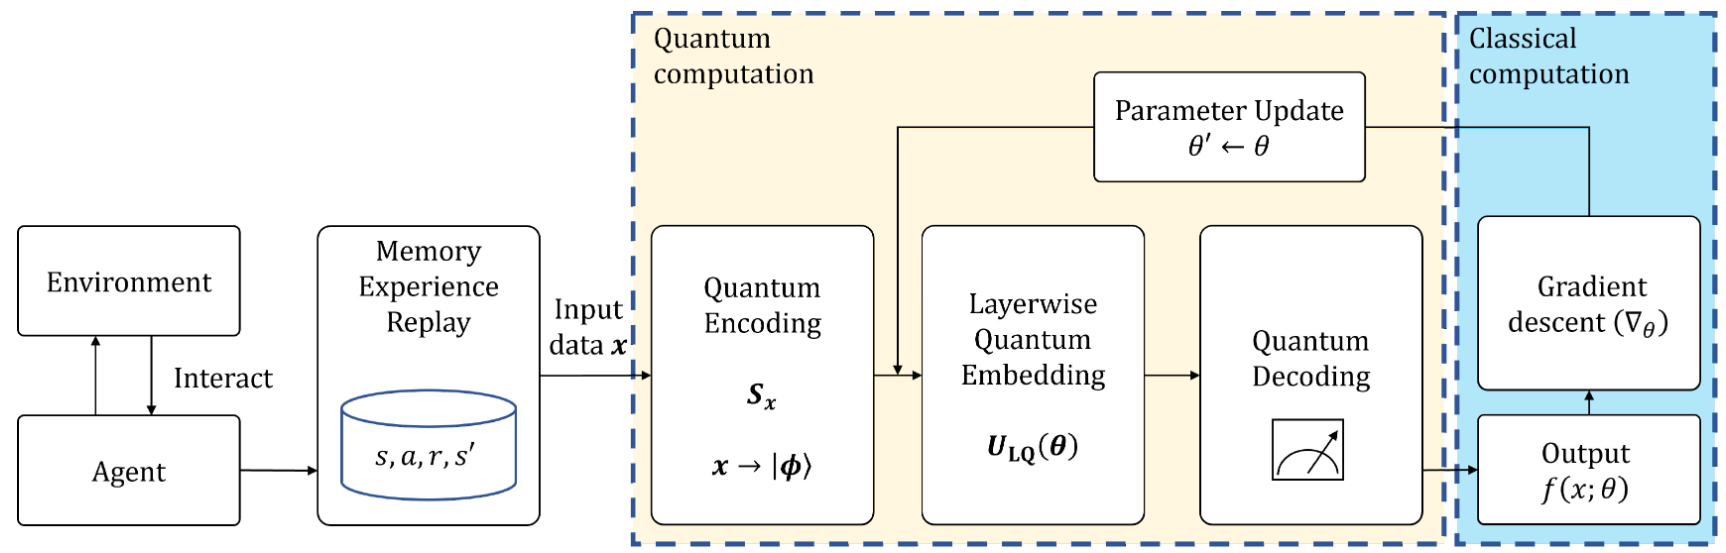
\includegraphics[width=1\textwidth]{figures/lq_drl_framework_silviratani_et_al.png}
    \caption{\acrshort{lqdrl} Framework Proposed by Silvirianti et. al (2025)}
    \label{fig:lqdrl_framework_silvirianti}
\end{figure}
It can be seen in Fig. \ref{fig:lqdrl_framework_silvirianti} that a hybrid approach is taken for computing the optimal parameters for the \acrshort{drl} algorithm, i.e., part of the computation is performed using quantum gates and the other part is performed using classical computing methods, however, both portions of the overall system rely on one another to perform \acrshort{drl}. 

The study involved the use of a \acrshort{drl} that employs a deep neural network to enable the agent to learn in a high-dimensional, continuous space and not a discrete one, which is typical for \acrshort{drl} algorithms. 

The optimal action policy is selected by the actor network and the critic network evaluates the quality of this selected policy by referring to the maximum Q-values at that given layer. The Q-values represent a value given a particular action and state at a given time.
As they are directly related to the rewards given for particular actions, they must be updated over time as opposed to being kept the same from iteration to iteration \cite{skolik_quantum_2022}. 

The use of quantum embedding and measurement for each layer was performed for encoding all of the data into quantum states with the use of an ansatz for quantum embedding, i.e. a quantum circuit. 
There is a decoding operator that acts on the quantum state for measurement to collapse the quantum information into classical information, which then provides an input for a gradient descent optimisation algorithm that updates parameters for the next layer to be embedded and subsequently decoded. 
The decoding operation is then used to calculate the value of the local loss for each iteration of this process and each measurement operation is performed $K_{shot}$ times. The local loss is a measure of the difference between the decoded output and the desired output averaged over $N_{data}$ times, where $N_{data}$ is the size of the encoded data. 

The proposed ansatz for the layerwise quantum embedding in this study is shown in Fig. \ref{fig:lqdrl_ansatz_silvirianti}, which has been reproduced from \cite{silvirianti_layerwise_2024}. 

\begin{figure}[ht]
    \centering
    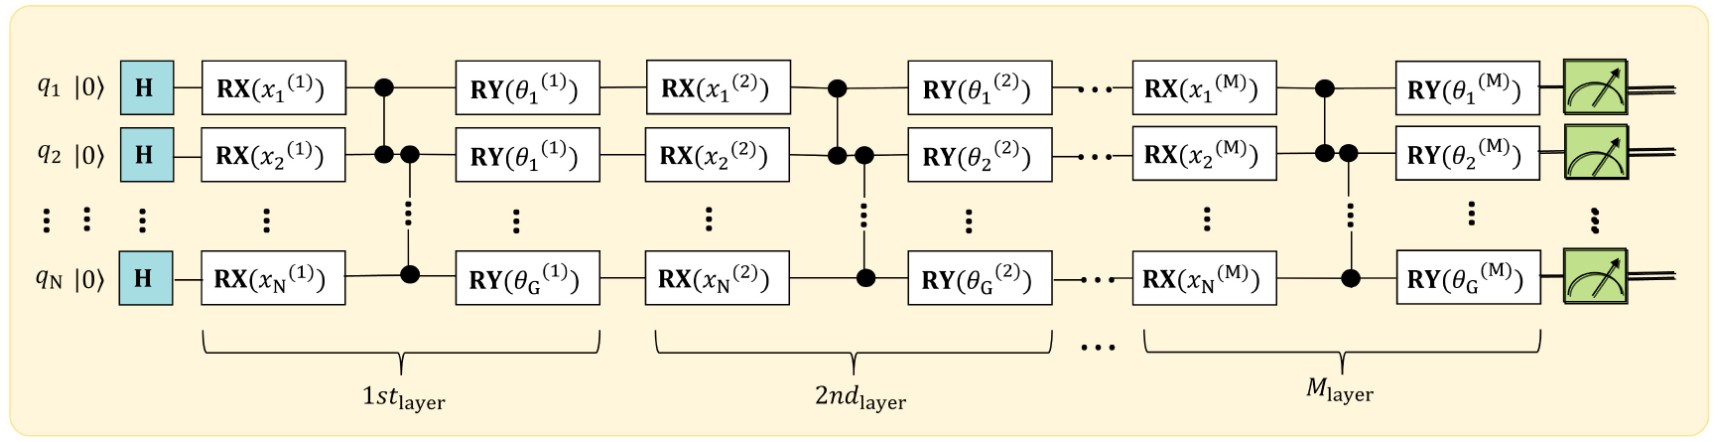
\includegraphics[width=1\textwidth]{figures/lq_drl_ansatz.png}
    \caption{Ansatz Used for Layerwise Quantum Embedding Proposed by Silvirianti et. al (2025)}
    \label{fig:lqdrl_ansatz_silvirianti}
\end{figure}
The layerwise quantum embedding process is performed for the actor and critic networks. 

The employed \acrshort{lqdrl} scheme was used to jointly optimise the \acrshort{uav} trajectory planning, transmit power allocation and \acrshort{noma} user grouping. 

The scenario considered for evaluating the performance of the algorithm involved a single \acrshort{uav} in three-dimensional space, with full power $E_{max}$, acting as an aerial \acrshort{bs} to provide downlink coverage serving $K$ \acrshort{gu}s that were distributed randomly over the horizontal plane, i.e. in two dimensions and moving at constant speeds.  
The authors formulated energy consumption models, \acrshort{noma} channel grouping, transmission power models, a noise and interference model and subsequently formulated an objective function that aimed to maximise the energy efficiency of the \acrshort{uav} network subject to the following constraints:
\begin{itemize}
    \item The total maximum transmit power of the \acrshort{uav} must not be exceeded by the total allocated power for the \acrshort{gu}s in a \acrshort{noma} group.
    \item The range of the allocated power coefficient for each user must not be exceeded and must fall between 0 and 1 .
    \item Higher transmission power must be allocated to \acrshort{gu}s with a lower channel gain.
    \item The minimum threshold data rate must be exceeded by the achievable data rate of any \acrshort{gu} within a given group at a particular time
    \item The \acrshort{uav} must remain within its maximum allowed co-ordinates in Cartesian co-ordinates.
\end{itemize}
The authors formulated a state space for the \acrshort{uav} in which the location, remaining energy to consume and the states of the \acrshort{gu}s are considered with $(2K + 4)$ state space dimensions, where $K$ denotes the number of \acrshort{gu}s. 

An action space was also formulated based on the objective problem of jointly optimising the \acrshort{uav} trajectory, \acrshort{noma} user grouping and power allocation. 
Action $a$ considered the following actions:
\begin{itemize}
    \item \textbf{\acrshort{uav} Trajectory} controlled by the velocity of the \acrshort{uav} and related to it's maneuvre.
    \item \textbf{\acrshort{noma} User Grouping} to address every possible GU clustering outcome and its objective is reward maximisation. 
    \item \textbf{Dynamic Power Allocation} which orders the transmit power allocations based on the highest to lowest channel gains for all of the \acrshort{gu}s.
\end{itemize}

The action space has 5 dimensions in total.

The reward $r$ is determined based on the energy efficiency $\eta(t)$ of a given episode and this is the value that's assigned as a reward if the energy efficiency optimisation is met, otherwise a value of $0$ is assigned for reward $r$. 

The \acrshort{lqdrl} algorithm used in \cite{silvirianti_layerwise_2024} demonstrated that the \acrshort{lqdrl} algorithm had higher effective dimensionality compared to a classical \acrshort{drl} approach. 
The layer loss was also shown to decrease in magnitude for each layer. 
The energy efficiency, critic and actor loss also decreased substantially, with improvements being demonstrated to occur for each layer. 
\chapter{Methodology}
\section{System Model \& Environment}
The proposed network architecture in use for this problem consists of a \acrshort{uav}-\acrshort{bs} for providing network coverage to a set of legitimate \acrshort{gu}s, in which physical layer security is upheld with the use of an \acrshort{ans} to mask the wireless signal from eavesdroppers attempting to perform \acrshort{mitm} attacks on legitimate communications links. 
A diagrammatic representation of the system architecture is shown in Fig. \ref{fig:mengsc_simplified_architecture}, with eavesdroppers referred to as "Eves" and the \acrshort{uav}-\acrshort{bs} shown to provide network coverage for a set of $\mathcal{K}$ legitimate \acrshort{gu}s.
\begin{figure}[ht!]
    \centering
    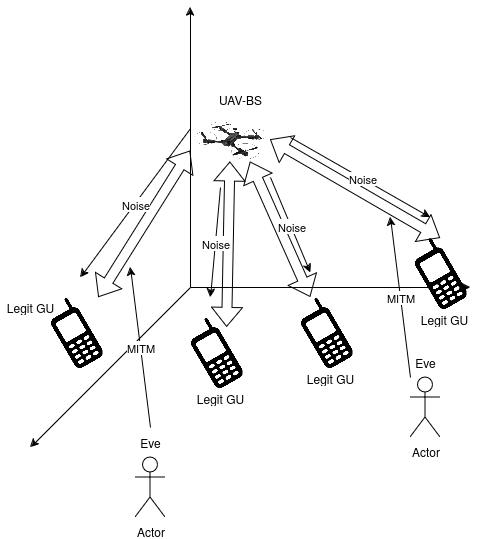
\includegraphics[width=0.7\textwidth]{figures/MEngSc_Thesis_system_architecture_updated.drawio.png}
    \caption{Simplified Diagram of the System Architecture}
    \label{fig:mengsc_simplified_architecture}
\end{figure}

Within the system architecture, there is a set $\mathcal{K}$ of K legitimate \acrshort{gu}s, a set $\mathcal{M}$ of E Eves and a set $\mathcal{X}$ of X \acrshort{uav}-\acrshort{bs}s. 
\subsection{\texorpdfstring{\acrshort{uav}-\acrshort{bs}}{UAV-BS}}
The purpose of the \acrshort{uav}-\acrshort{bs}s are to establish and maintain \acrshort{uav}-\acrshort{gu} communication links with legitimate \acrshort{gu}s while ensuring those communications are physically secure and maintaining an acceptable secrecy rate.  
They provide network coverage to the \acrshort{lu}s and their trajectory, data rate of exchange, energy efficiency and secrecy rate must be optimised to ensure the delivery of adequately secure and energy-efficient communication links for legitimate \acrshort{gu}s. 
The mobility model for the \acrshort{uav} is shown in \ref{eq:uav_mobility_model} \cite{silvirianti_layerwise_2024}. 
\begin{equation} \label{eq:uav_mobility_model}
   v_{\acrshort{uav}} (t) = \delta V_{max}, \ 0 < \delta \le 1
\end{equation}
In this model, the \acrshort{uav}-\acrshort{bs}s can only be connected to the legitimate \acrshort{gu}s and must generate an \acrshort{ans} to combat eavesdropping from Eves based on their observed positions. 
\subsection{Legitimate \texorpdfstring{\acrshort{gu}s}{GUs}}
The \acrshort{lu}s within the system model are the \acrshort{gu}s that the \acrshort{uav}-\acrshort{bs} wishes to communicate with secrectly. 
This involves the \acrshort{lu} having to receive a noisy signal that contains the desired modulated data for the \acrshort{lu} with an \acrshort{ans} that the \acrshort{lu} is provided with information about to enable the \acrshort{lu}'s receiver to filter the \acrshort{ans} from the signal. 
\subsection{Eavesdroppers}
The Eves within the system are eavesdroppers that wish to perform \acrshort{mitm} attacks by detecting and storing the \acrshort{uav}-\acrshort{lu} communications data. 
With the Eves in the environment, they have an eavesdropping rate $R_{E, k} (t), \forall \ k$ for each of the K \acrshort{lu}s which describes how much data they are managing to intercept and store between the \acrshort{uav}-\acrshort{bs} and any of the \acrshort{lu}s. 
The \acrshort{uav}-\acrshort{bs} must estimate the worst-possible value for $R_{E, k} (t)$ to inject \acrshort{ans} into the modulated waveform that minimises the \acrshort{snr} for all E $\in \mathcal{M}$ Eves. 
\subsection{\texorpdfstring{\acrshort{noma}}{NOMA} Communications Model}
A \acrshort{noma} communication scheme has been chosen as it offers potentially higher data exchange rates and all \acrshort{gu}s can be communicated with by the \acrshort{uav}-\acrshort{bs} using a \acrshort{mimo} antenna array on the \acrshort{uav} without the need for division of frequency or time for multiple \acrshort{gu}s to communicate with the \acrshort{uav}. 
The transmitted signal using \acrshort{noma} is shown in \ref{eq:tx_signal_noma} and the received signal is shown in \ref{eq:rx_signal_noma} \cite{silvirianti_layerwise_2024, bizaki_towards_2016}. 
\begin{equation} \label{eq:tx_signal_noma}
    x_{n} = \sum_{k=1}^{K} \sqrt{P_{k, n}^{Tx}} s_{k}
\end{equation}
\begin{equation} \label{eq:rx_signal_noma}
   y_{n} = h_{k, n} (t) x_{n} + I_{k, n}
\end{equation}
In \ref{eq:tx_signal_noma}, $P_{k, n}^{Tx}$ refers to the transmitted signal power and $s_k$ refers to the modulated symbols being transmitted. 
In \ref{eq:rx_signal_noma}, $h_{k, n}$ is the channel gain and $I_{k, n}$ is the interference in the channel caused by the other \acrshort{gu}s being communicated to be the \acrshort{uav}-\acrshort{bs}. 
$I_{k, n}$ in \ref{eq:rx_signal_noma} is removed from the received signal with the use of \acrfull{sic}. 

\subsection{Rician Channel Model \& Environmental Considerations}
The Rician channel model describes a communications channel in which the propagating waveform is made up of a dominant \acrshort{los} path between the receiver and transmitter as well as non-dominant paths. 
The channel model can be characterised with the use of Rician K-factors and $\Omega$-factors \cite{rice_statistical_1948}, shown in \ref{eq:rician_k_factor} and \ref{eq:rician_omega_factor}. 
Rician K-factors describe the ratio of the dominant signal power to the non-dominant signal power in a communication channel. 
The $\Omega$-factors act as a scaling factor for the Rician distribution and is the sum of the dominant and scattered paths. 
%\begin{equation} \label{eq:cosine_wave}
%    s(t) = cos(\omega_{c}t)
%\end{equation}
\begin{equation} \label{eq:dom_and_non_dom_signal}
    v(t) = C \cdot cos(\omega_{c}t) + \sum_{n=1}^{N} r_n cos(\omega_{c}t + f_n)
\end{equation}
\begin{equation} \label{eq:rician_k_factor}
    K = \frac{v^{2}}{2\sigma^{2}}
\end{equation}
\begin{equation} \label{eq:rician_omega_factor}
    \Omega = v^{2} + 2\sigma^{2}
\end{equation} 

The K-factors are computed dynamically with the use of channel gain coefficients that are fixed parameters of the channel, $A_{1}$ and $A_{2}$. 
The elevation angle, $\theta$ between the \acrshort{uav}-\acrshort{bs} and a given \acrshort{gu} is given by \ref{eq:rician_theta} \cite{you_3d_2019}.
\begin{equation} \label{eq:rician_theta}
   \theta = \sin^{-1}\begin{pmatrix}
       \frac{z_{U}}{d_{U}} 
   \end{pmatrix}
\end{equation}
\begin{equation} \label{eq:dynamic_k_factor}
    K = A_{1} e^{A_{2} \theta}
\end{equation}
\begin{equation} \label{eq:rician_g_val}
    g_{U}[k] = \sqrt{\frac{K}{1+K}} g + \sqrt{\frac{1}{K+1}} \tilde{g}
\end{equation}
\begin{equation} \label{eq:pathloss_equation}
   \zeta_{k, n}^{fs} = 20\log_{10}(d_{U} [k]) + 20\log_{10}(f_{c}) + 20\log_{10} \begin{pmatrix}
       \frac{4\pi}{c}
   \end{pmatrix}
\end{equation}
\begin{equation} \label{eq:dynamic_rician_gain}
   h_{U} [k] = g_{U} [k] d_{U} [k]^{-\zeta_{k, n}}
\end{equation}
In \ref{eq:rician_g_val}, $g$ is the deterministic \acrshort{los} component and $\tilde{g}$ is the \acrfull{nlos} random scattered components, which is represented as a \acrfull{cscg}. 
The \acrfull{fspl} exponent shown in \ref{eq:pathloss_equation} in dB, $\zeta_{k, n}$ and $f_{c}$ refers to the carrier frequency of the waveform and $c$ refers to the speed of light. 
The channel gain $h_{U} [k]$ shown in \ref{eq:dynamic_rician_gain} is a function of \ref{eq:rician_g_val}, \ref{eq:pathloss_equation} and $d_{U} [k]$ \cite{li_joint_2024}. 

\section{Mathematical Derivations \& Problem Definition}
The desired outcome of the algorithm and overall system involving \acrshort{uav}s as networking platforms is that the \acrshort{uav}s acting in the environment can perform their task of providing optimal network coverage that must be energy efficient, secret and secure for legitimate \acrshort{gu}s while also ensuring that eavesdropping \acrshort{gu}s are prevented from eavesdropping on legitimate \acrshort{uav}-\acrshort{gu} communications. 
The maximisation of the secrecy rate is a joint optimisation problem that is reliant on the maximisation of the energy efficiency, the maximisation of the data exchange rate, the optimisation of the data exchange rate and the minimisation of the \acrshort{uav} trajectory. The definitions and explanations for these optimisation problems are outlined in the following subsections. 
\subsection{Secrecy Rate Optimisation}
The secrecy rate optimisation is derived from the \acrshort{noma} data exchange rate optimisation, energy efficiency optimisation and the \acrshort{uav} trajectory optimisation. 

The secrecy rate, with aspects adapted from \cite{zhang_one_2025}, with the model for \acrshort{noma} communications from \cite{silvirianti_layerwise_2024}, is derived from the subchannel bandwidth, which allocates a frequency band from the total carrier frequency bandwidth at a given time in which a portion of the total transmit power is allocated to each \acrshort{gu} based on each of their respective channel gains, $h_{U, k}$.
\begin{equation} \label{eq:noma_subchannel_bw}
   \sum_{k=1}^{K} B_{sc} \le BW_{f_{c}}
\end{equation}
As shown in \ref{eq:noma_subchannel_bw}, the sum of the subchannel bandwidths must not exceed the total bandwidth of the carrier frequency $f_{c}$. 

The position of the \acrshort{uav} must only change such that it cannot exceed the maximum step change, $\delta$ multiplied by the maximum velocity of the \acrshort{uav}, $V_{max}$. 

Equation \ref{eq:uav_power_constraint} shows the allocated transmit power cannot exceed the maximum allocated power in timeslot $n$. 
\begin{equation} \label{eq:uav_power_constraint}
    \sum_{i=0}^{I} P_{U, i} [n] \le P_{U, k}^{Tx} [n], \forall n
\end{equation}
The distance between the \acrshort{uav} and \acrshort{gu}, shown in \ref{eq:distance_uav_gu} is factored into the channel gain along with the directional gain of the antennae on the \acrshort{uav} and the \acrshort{gu}. 
This \acrshort{uav} channel gain $h_{U, k}$ for $k$ \acrshort{gu}s, shown in \ref{eq:channel_gain_uav_gu} is subsequently used in \ref{eq:snr_uav_gu} for computing the data rate in the \acrshort{uav}-\acrshort{gu} communications channel, which in turn, is used to compute the \acrshort{masr} or the secrecy rate of the communications. 

\begin{equation} \label{eq:distance_uav_gu}
    d_{U, k} = \sqrt{(x_{U, k}-x_{GU, k})^2 + (y_{U, k}-y_{GU, k})^2 + (z_{U, k}-z_{GU, k})^2}
\end{equation}
\begin{equation} \label{eq:channel_gain_uav_gu}
    h_{U, k} [n] = g_{U, k} [n] d_{U, k} [n]^{-\zeta_{k, n}}
    %h_{U, k} = \frac{G_{0}G_{1}\beta_{0}}{(d_{U, k}[n])^2}
\end{equation} 
\begin{equation} \label{eq:snr_uav_gu}
    \acrshort{snr}: \gamma_{U, k, i} [n] = \frac{P_{U, i}[n] h_{U, k}[n]}{I_{k, n} + (\sigma_{\acrshort{los}} + \sigma_{\acrshort{nlos}} + \sigma_{\acrshort{awgn}})^{2}}
    %\acrshort{snr}: \gamma_{U, k, i} [n] = \frac{P_{U, i}[n] h_{U, k}[n]}{B_{0}N_{0}^{GU}}
\end{equation} 
The \acrshort{snr} is the ratio of the channel power by the channel gain to the sum of the \acrshort{awgn}, \acrshort{los} and \acrshort{nlos} noise power values and $I_k, n$ is the interference from other users, which is canclled with \acrshort{sic}. 
The rate of data exchange in the \acrshort{uav}-\acrshort{gu} communication link is expressed in \ref{eq:uav_gu_data_rate}, which is a function of the subchannel bandwidth $B_{sc} [n]$ in slot $[n]$ and the \acrshort{snr}. 
\begin{equation} \label{eq:uav_gu_data_rate}
    R_{U, m, i} [n] = B_{sc}[n] \log_{2} (1 + \gamma_{U, m, i}[n]), \forall i, m, n
\end{equation} 
The position of Eve $m$ in timeslot $n$ is shown in \ref{eq:exact_eve_position}. 
\begin{equation} \label{eq:exact_eve_position}
    s_{m} [n] = \begin{pmatrix}
        x_{m} [n] & y_{m} [n] & z_{m} [n]
    \end{pmatrix} ^{T}
\end{equation}
The \acrshort{uav}-\acrshort{bs} observes the state with all of the \acrshort{gu}s, and those that have not been authenticated as \acrshort{lu}s within the network are classed as Eves. 
Based on the proximity of the perceived Eves within the environment, the \acrshort{uav}-\acrshort{bs} must calculate the eavesdropping rate that each Eve has for each \acrshort{lu} as shown in \ref{eq:eavesdropping_rate_eq}. 
\begin{equation} \label{eq:eavesdropping_rate_eq}
   R_{E, k, m} [n] = B_{sc} [n] \log_{2} (1 + \gamma_{E, k, n} [n]), \forall \ k, m, n
\end{equation}
The eavesdropping rates with the highest values are used for the calculation of the \acrshort{ans}. 
With this secrecy scheme, each of the \acrshort{lu}s are protected from the worst-case eavesdropping rate, i.e., the eavesdropping rate of whichever Eve has the greatest \acrshort{snr} to conduct their \acrshort{mitm} attack. 
%The estimated position of Eve $m$ is $\tilde{s}_{m}$, which is a circle of radius $\mathcal{E}$ with estimation errors $\Delta x_{m} [n], \Delta y_{m} [n] \in \mathcal{E}$. 
%The relationship between the exact and estimated Eve position is shown in \ref{eq:estimated_eve_position_x} and \ref{eq:estimated_eve_position_y}. 
%\begin{equation} \label{eq:estimated_eve_position_x}
%    x_{m} [n] = \tilde{x}_{m} [n] + \Delta x_{m} [n]
%\end{equation}
%\begin{equation} \label{eq:estimated_eve_position_y}
%    y_{m} [n] = \tilde{y}_{m} [n] + \Delta y_{m} [n]
%\end{equation}
%The actual Eve position is within a circle of radius $\tilde{s}_{m} [n]$ with a radius of $\mathcal{E}$ such that $\mathcal{E} \le ||q_{U}[n] - \tilde{s}_{m} [n]||$. 
The worst-case eavesdropping rate is shown in \ref{eq:worst_case_eve_rate} and the minimum secrecy rate is expressed in \ref{eq:secrecy_rate}, being the absolute difference between \ref{eq:uav_gu_data_rate} and \ref{eq:worst_case_eve_rate} \cite{zhang_one_2025}. 
The secrecy sum rate is expressed in \ref{eq:secrecy_sum_rate}
%\begin{equation}\label{eq:worst_case_eve_rate}
%    \Phi = \underset{\mathcal{M}}{\max}\begin{Bmatrix} \underset{\Delta x_{m} [n], \Delta y_{m} [n] \in X}{\max} 
%        R_{E, k, m}[n]
%    \end{Bmatrix}, \forall k, m, n
%\end{equation} 
\begin{equation}\label{eq:worst_case_eve_rate}
    \Phi = \underset{\mathcal{M}}{\max}\begin{Bmatrix} \underset{\max \gamma_{E, k, m}[n]}{\max} 
        R_{E, k, m}[n]
    \end{Bmatrix}, \forall k, m, n
\end{equation} 
\begin{equation} \label{eq:secrecy_rate}
    R_{k, i}^{sec} [n] = [R_{U, k, i} [n] - \Phi]^{+}, \forall i, k, n
\end{equation} 
\begin{equation} \label{eq:secrecy_sum_rate}
    \bar{R}_{k, i}^{sec} [n] = \frac{1}{N} \sum_{n=1}^{N} \sum_{i=1}^{I} R_{k, i}^{sec} [n], \forall k
\end{equation}
%\hl{REWRITE THIS PORTION WITH PROPER EQUATION REFERENCING FOR THE CONSTRAINTS AND OBJECTIVE FUNCTION} 

The secrecy rate is to be maximised subject to the following constraints, the \acrshort{uav} must not exceed its range and altitude limits in three-dimensional Cartesian space (\ref{eq:secrecy_rate_position_constraint}), the power consumption must not exceed the maximum power consumption over time (\ref{eq:secrecy_rate_power_constraint}), the allocated transmit power must be greater than or equal to 0 (\ref{eq:secrecy_rate_tx_power_constraint}) and the change in position of the \acrshort{uav} must not exceed the step size $\delta$ multiplied by the maximum velocity of the \acrshort{uav}, $V_{max}$ (\ref{eq:secrecy_rate_trajectory_constraint}). 
The co-ordinate position of the \acrshort{uav} in Cartesian co-ordinates, $[x_{U}, y_{U}, z_{U}]$ is denoted as $q_{U}$ in \ref{eq:secrecy_rate_trajectory_constraint}.
\begin{equation} \label{eq:secrecy_rate_objective_function}
    \underset{q_{U}, A, E, Q}{\max}\bar{R}_{k, i}^{sec}, s.t.
\end{equation} 
\begin{equation} \label{eq:secrecy_rate_power_constraint}
    \sum_{i=1}^{I} P_{U, i} \le P_{tot}
\end{equation}
\begin{equation} \label{eq:secrecy_rate_tx_power_constraint}
    0 \le P_{U, k}^{Tx} \le P_{U_{tot}}^{Tx}, \forall k
\end{equation}
\begin{equation} \label{eq:secrecy_rate_subchannel_constraint}
    \sum_{k=1}^{K} B_{sc, k} [n] \le BW_{f_c}, \forall \ k
\end{equation}
\begin{equation} \label{eq:secrecy_rate_e_cons_constraint}
    E_{cons} \le E_{max}
\end{equation} 
\begin{equation} \label{eq:secrecy_rate_trajectory_constraint}
    ||q_{U}[n+1] - q_{U}[n]||^2 \le (\delta V_{max})^2, \forall \ n
\end{equation} 
\begin{equation} \label{eq:secrecy_rate_position_constraint}
    x_{min} \le x_{U} \le x_{max}
    ,\  
    y_{min} \le y_{U} \le y_{max}
    ,\  
    z_{min} \le z_{U} \le z_{max}
\end{equation}
The subchannel allocation, \acrshort{uav} trajectory and energy efficiency must be maximised as part of this joint optimisation problem to ensure that the secrecy rate is maximised. 
The Eve \acrshort{snr} must also be minimised in order to minimise the eavesdropping rate, as described in \ref{eq:maximise_eve_snr_constraint} and \ref{eq:minimise_eve_rate_constraint}. 
The maximisation of the \acrshort{uav}-\acrshort{lu} data rate is also required to minimise the eavesdropping rate and the maximisation of the \acrshort{ans}, $\psi$. 
\begin{equation} \label{eq:maximise_eve_snr_constraint}
   \underset{\psi}{\max}\gamma_{E, m, k}
\end{equation}
\begin{equation} \label{eq:minimise_eve_rate_constraint}
   \underset{\min \gamma_{E, k, m}}{\min} R_{E, k, m} [n], \forall \ k, m, n
\end{equation}
\subsection{Energy Efficiency Optimisation}
The energy consumption mathematical model has been adapted from \cite{silvirianti_layerwise_2024} to describe the consumption of energy on board any given \acrshort{uav}. The model accounts for the energy consumed while travelling, hovering, by the avionics and the communication energy. 
The energy consumption at time $t$, $E_{cons}(t)$ can be expressed as shown in \ref{eq:energy_cons_model}.

%\hl{CHANGE THE MASS CALCULATION AS IT SHOULD BE A CONSTANT. NO CLEAR REASON TO SUM IT TWICE}
\begin{equation} \label{eq:energy_cons_model}
    E_{cons}(t) = \sum_{n=1}^{N} \sum_{k=1}^{K_n} \left (\underbrace{\frac{\sum_{i=1}^{I} n_{i} g |q_{U}(t)|}{K\textit{r}}}_{\text{Travelling}} + 
    \underbrace{\frac{((\sum_{i=1}^{I}n_i)g)^{\frac{3}{2}}}{\sqrt{2 r \zeta \theta}}}_{\text{Hovering}} +
    \underbrace{\Lambda \frac{|q_{U}(t)|}{v(t)}}_{\text{Avionics}} + 
    \underbrace{P_{k, n}^{Tx}(t) R_{k, n}(t)}_{\text{Communications}} \right)
\end{equation}
In \ref{eq:energy_cons_model}, $n_{i}$ is the mass of the \acrshort{uav} frame and battery, $g$ is acceleration due to gravity ($9.81\ m s^{-2}$), $q_{U}(t)$ is the position of the \acrshort{uav} at time $t$, $K$ is the lift-to-drag ratio, shown in \ref{eq:lift_to_drag_ratio}, $r$ denotes the number of \acrshort{uav} rotors, $\zeta$ refers to the air density, $\theta$ is the spinning blade of a single rotor, $\Lambda$ is the avionics power and $v(t)$ is the velocity of the \acrshort{uav} at time $t$ \cite{silvirianti_layerwise_2024, zhang_energy_2021}. 

%\hl{POSSIBLE NEED TO UPDATE LIFT TO DRAG RATIO HERE FOR QUADCOPTER UAV}
\begin{equation} \label{eq:lift_to_drag_ratio}
   K = \frac{L}{D} = \frac{\sum_{i=1}^2 n_{i} g v_{U}}{P}
\end{equation}
$\sum_{i=1}^2 n_{i}$ is the mass of the \acrshort{uav} frame and battery, $g$ is the acceleration due to gravity, $v_{U}$ is the velocity of the \acrshort{uav} and $P$ is the power required for the \acrshort{uav} \cite{theys_forward_2020}. 
%\begin{equation} \label{eq:lift_to_drag_ratio}
%    K = \left (\frac{L}{D} \right )_{max} = \frac{1}{2} \sqrt{\frac{\pi \epsilon (AR)}{C_{D, 0}}}
%\end{equation}
%Where $\epsilon$ is the span efficiency factor, $AR$ refers to the aspect ratio of the \acrshort{uav} wings and $C_{D, 0}$ is the zero-lift drag coefficient. \hl{CITATION}

As can be seen in the expression for the communications energy, the transmit power is included within the energy consumption model, which is factored into the secrecy rate in \ref{eq:secrecy_rate_objective_function}.
The total energy efficiency can be expressed as shown in \ref{eq:energy_efficiency}. 
\begin{equation} \label{eq:energy_efficiency}
    \eta (T) = \int_{t=1}^{T} \frac{\sum_{n=1}^{N} \sum_{k=1}^{K_{n}} R_{k, n}(t)}{E_{cons}(t)} dt
\end{equation}
The energy efficiency must be maximised as part of the joint optimisation expressed in \ref{eq:secrecy_rate_objective_function}. The optimisation of \ref{eq:energy_efficiency} is detailed in \ref{eq:energy_efficiency_objective_function} and the maximisation of $\eta(t)$ involves the optimisation of the user grouping, \acrshort{uav} position and power allocation on the \acrshort{uav}. 
\begin{equation} \label{eq:energy_efficiency_objective_function}
    \underset{G_{n} \in N, q_{U}(t), P_{k, n}^{Tx}(t)}{\max} \eta (t), s.t.
\end{equation}
\begin{equation} \label{eq:energy_efficiency_transmit_power_constraint}
    \sum_{n=1}^{N} \sum_{k=1}^{K_n} P_{k, n}^{Tx} \le P_{UAV}^{Tx} 
\end{equation}
\begin{equation} \label{eq:energy_efficiency_power_coefficient_constraint}
    0 < \sum_{k=1}^{K_n} a_{k, n} \le 1
\end{equation}
\begin{equation} \label{eq:energy_efficiency_power_coefficient_order_constraint}
    a_{1, n} < \dots < a_{K_n, n}
\end{equation}
\begin{equation} \label{eq:energy_efficiency_transmit_rate_coefficient}
    R_{k, n} [n] \ge R_{min}
\end{equation}
\begin{equation} \label{eq:energy_efficiency_position_constraint}
    x_{min} \le x_{U} \le x_{max},\ y_{min} \le y_{U} \le y_{max},\ z_{min} \le z_{U} \le z_{max}
\end{equation}
The constraints applied to \ref{eq:energy_efficiency_objective_function} include the limit of the maximum transmit power in a \acrshort{noma} group of \acrshort{gu}s (\ref{eq:energy_efficiency_transmit_power_constraint}), the transmit power coefficient range for each \acrshort{gu} (\ref{eq:energy_efficiency_power_coefficient_constraint}), the fact that each transmit power coefficient must be ordered such that a higher coefficient is granted to users with a lower channel gain (\ref{eq:energy_efficiency_power_coefficient_order_constraint}), the transmitted data rate must exceed the minimum threshold data rate (\ref{eq:energy_efficiency_transmit_rate_coefficient}) and the \acrshort{uav} must remain within the bounds of its range and altitude (\ref{eq:energy_efficiency_position_constraint}). 

%\subsection{\acrshort{ofdm} Channel Subcarrier Allocation Optimisation}
%\hl{CHANGE THIS TO NOMA DATA RATE OPTIMISATION AS NOMA IS BEING USED IN THE MODEL}
%
%The \acrshort{ofdm} subcarrier channels are a resource for the \acrshort{uav}-\acrshort{bs} to allocate for a given legitimate \acrshort{gu} and they are scheduled such that the subcarrier channel allocation is fair for all \acrshort{gu}s and provides a reasonable \acrfull{qos}. 
%\acrshort{ofdm} is in use due to its high spectral efficiency and resilience to noisy channels. 
%Each subcarrier can be described as shown in \ref{eq:ofdm_subcarrier_wave}. 
%\begin{equation} \label{eq:ofdm_subcarrier_wave}
%    s_{c}(t) = A_{c} e^{j|\omega_{c} + \phi_{c}(t)|}
%\end{equation}
%Where $A_{c}$ is the symbol of the carrier and its magnitude, while $s_{c}(t)$ is a complex wave containing both a magnitude and phase. 
\subsection{Optimisation of \texorpdfstring{\acrshort{uav}-\acrshort{gu}}{UAV-GU} Data Exchange Rate}
As the function of data rate exchange shown in \ref{eq:uav_gu_data_rate} is a function of the \acrshort{snr}, which itself is a function of the channel gain, which is dependent on the distance between the \acrshort{uav}-\acrshort{bs} and any given \acrshort{gu} as a result of the \acrshort{fspl}, the \acrshort{uav}-\acrshort{gu} data exchange rate can be optimised by minimising the distance between the \acrshort{uav}-\acrshort{bs} and all $K$ \acrshort{gu}s. 
To achieve \ref{eq:data_rate_objective_function}, the difference in distances between all \acrshort{gu} to the \acrshort{uav}-\acrshort{bs} must be minimised and the distance between the \acrshort{uav}-\acrshort{bs} to the \acrshort{gu} centroid must be minimised. 
The differences in distances between the \acrshort{uav}-\acrshort{bs} and the \acrshort{gu}s is expressed in \ref{eq:gu_dist_diffs}. 
Minimising this distance as shown in \ref{eq:min_gu_dist_diffs} ensures that all \acrshort{gu}s are receiving a level of network coverage that is above $R_{min}$.
Minimising the distance between the \acrshort{uav}-\acrshort{bs} helps to ensure that the \acrshort{uav} trajectory is optimised, as shown in \ref{eq:uav_trajectory_objective_function}, while also maximising $R_{U, k} [n]$, as expressed in \ref{eq:data_rate_objective_function}. 
The \acrshort{gu} centroid, $C_{GU} [n]$ is the average value between all of the \acrshort{gu} positions. 
\begin{equation} \label{eq:data_rate_objective_function}
    \max R_{U, k} [n]
\end{equation}
\begin{equation} \label{eq:gu_dist_diffs}
    \lambda_{GU} [n] = \sum_{k=1}^{K} \sum_{j \neq k}^{K} |d_{U, k} [n] - d_{U, j}[n]|
\end{equation}
\begin{equation} \label{eq:min_gu_dist_diffs}
    \min \lambda_{GU} [n]
\end{equation}
\begin{equation} \label{eq:gu_centroid}
    C_{GU} [n] = \frac{1}{K} \sum_{k=1}^{K} d_{U, k} [n] + z_{min}
\end{equation}
\begin{equation} \label{eq:min_gu_centroid}
    \min C_{GU} [n]
\end{equation}
The objective functions shown in \ref{eq:data_rate_objective_function}, \ref{eq:min_gu_dist_diffs} and \ref{eq:min_gu_centroid} are subject to the constraints shown in \ref{eq:secrecy_rate_trajectory_constraint}, \ref{eq:secrecy_rate_position_constraint}, \ref{eq:energy_efficiency_transmit_power_constraint} and \ref{eq:energy_efficiency_transmit_rate_coefficient}.  

\subsection{Optimisation of \texorpdfstring{\acrshort{uav}}{UAV} Trajectory}
The \acrshort{uav} trajectory can be expressed as \ref{eq:uav_trajectory}.
\begin{equation} \label{eq:uav_trajectory}
   c(t) = q_{U}[n+1] - q_{U}[n]
\end{equation}
The trajectory is to be minimised such that the \acrshort{uav} can take the shortest path to serve its role for a set of $K$ \acrshort{gu}s and other \acrshort{uav}s. 
\begin{equation} \label{eq:uav_trajectory_objective_function}
   \underset{}{\min}\ q_{U}(t), s.t.
\end{equation}
\begin{equation}\label{eq:traj_boundary_constraints}
    x_{min} \le x_{U} \le x_{max},\ y_{min} \le y_{U} \le y_{max},\ z_{min} \le z_{U} \le z_{max}
\end{equation}
\begin{equation} \label{eq:distance_constraint}
    d_{U}, k \le 100, \forall k
\end{equation}
\section{Algorithms \& System Design}
%\hl{TODO: UPDATE THIS TO REFLECT THAT ONLY ONE UAV-BS WILL BE IN USE (AT LEAST AT PRESENT)}
The proposed approach for solving the outlined optimisation problem leverages \acrshort{drl} to determine the optimal secrecy rate for \acrshort{uav}-\acrshort{gu} communications such that $R_{U, k, n} \forall k, n$ over \acrshort{noma} is optimised, the energy efficiency converges to higher values, the resource allocation is optimised and the \acrshort{uav} trajectories are optimised. 
%A \acrshort{ppo}-based algorithm is used for this problem and solved in the classical computation case and a subsequent implementation of this algorithm, where part of the computation is offloaded to a gate-based quantum computer is also outlined. 
\subsection{Design}
The overall architecture of the system is illustrated in Fig. \ref{fig:system_block_diagram}. 

\begin{figure} [ht!]
    \centering
    %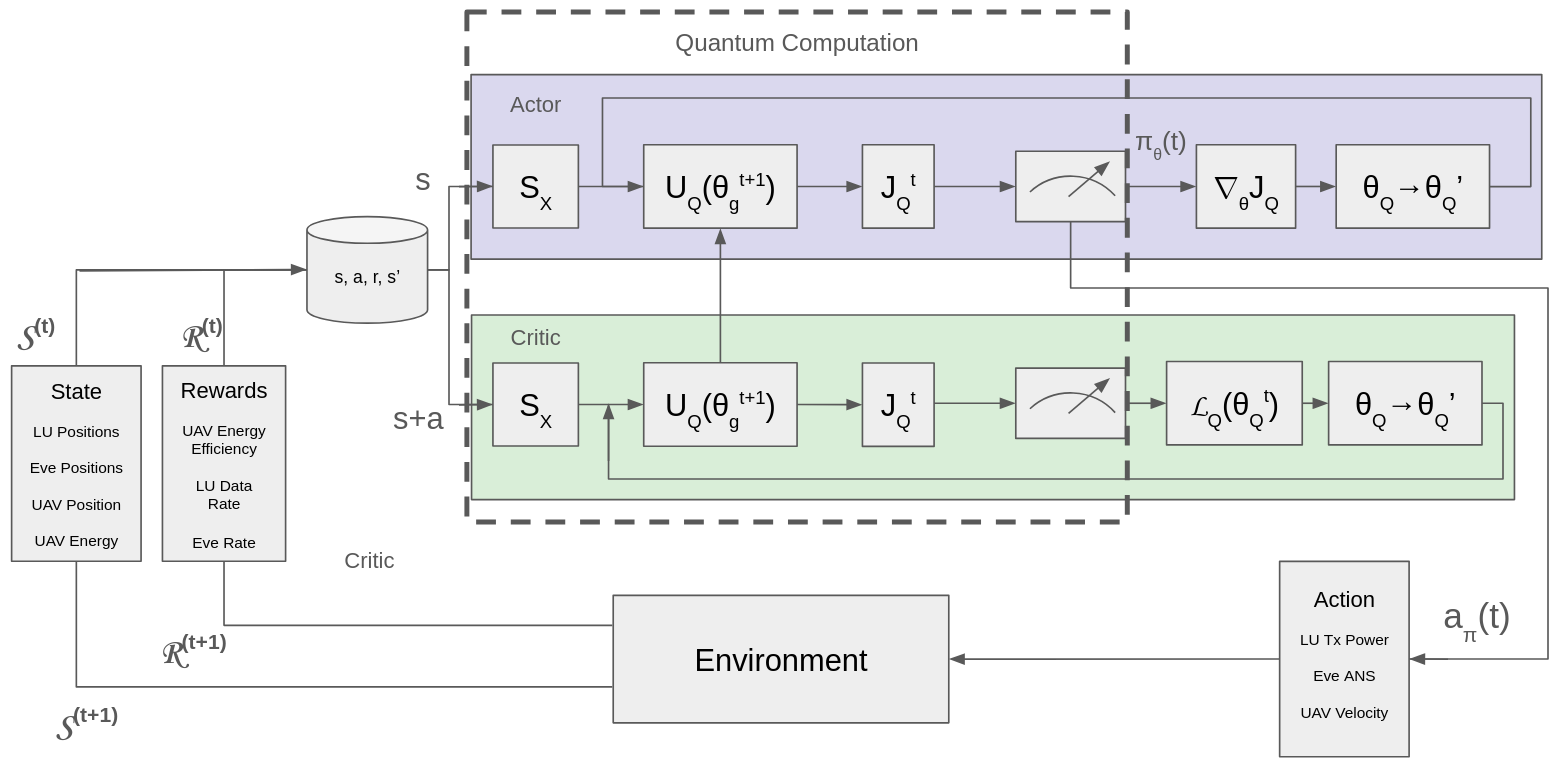
\includegraphics[width=1\textwidth]{figures/annotated_system_block_diagram.png}
    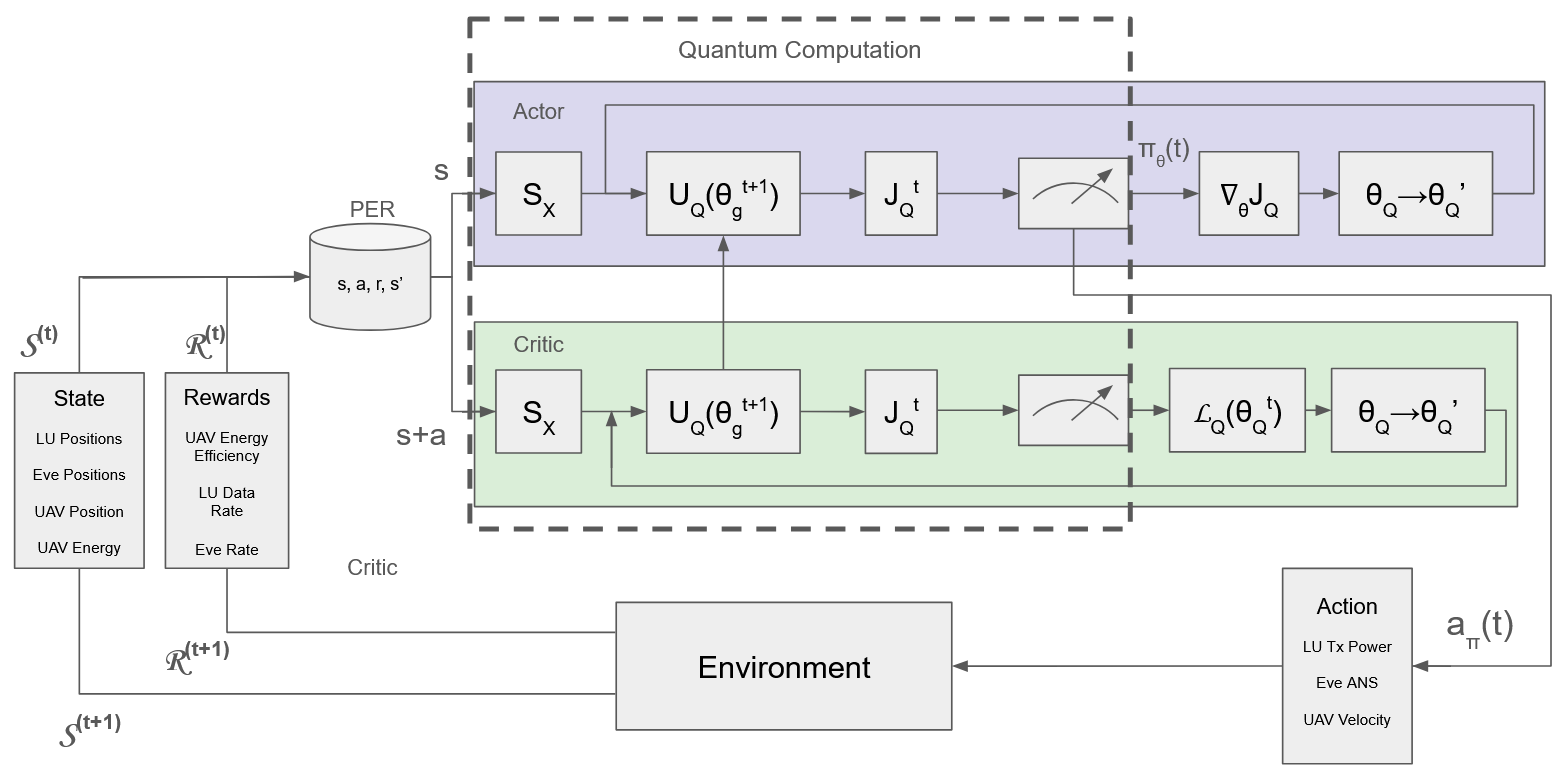
\includegraphics[width=1\textwidth]{figures/system_block_diagram_labelled.png}
    \caption{System Block Diagram}
    \label{fig:system_block_diagram}
\end{figure}
As shown in Fig. \ref{fig:system_block_diagram}, the overall system is a quantum-classical hybrid approach to the joint optimisation problem outlined in the previous section of this chapter. 
This system architecture has been adapted from \cite{silvirianti_layerwise_2024} and \cite{silvirianti_uav_2024}.
The design of the \acrshort{lqdrl} algorithm employing layerwise quantum embedding involves the use of storing parameters of the system as quantum states using a quantum circuit, referred to as an ansatz. 
This process is referred to as quantum encoding. 
The input parameter data is stored in a vector $\textbf{x}$ of $N$ elements, which are encoded into a set of quantum states $\ket{\phi}_{0, 1, \dots, N-1}$. 
The encoding process is denoted as $S_{\textbf{x}}$. 
The \acrshort{uav} is an agent interacting with the environment to observe the state space $s$, determine an action $a$ that is best in line with the desired policy $\pi$ that yields a reward $r$ and creates the updated state space $s'$. 
These parameters are embedded within the ansatz as $N$ qubits, where $N$ denotes the number of parameters required for the quantum data embedding. 
The value function of the selected policy $\pi$ for a state $s$ is shown in \ref{eq:policy_value_function} and $\mu'$ is the learning discount rate \cite{murphy2025reinforcementlearningoverview}. 
\begin{equation} \label{eq:policy_value_function}
   V_{\pi} (s) = E \begin{pmatrix}
       \sum_{t=1}^{T} \mu' r_{t} | s_{0}=s
   \end{pmatrix} 
\end{equation}
The system has been designed as a \acrfull{dqn}. 
Q-learning involves evaluating the quality or value of a state/action pair by determining it's Q-value $Q(s, a)$. 
The Q-value can be updating as shown in \ref{eq:q_value_update} \cite{murphy2025reinforcementlearningoverview}. 
\begin{equation} \label{eq:q_value_update}
   Q^{update} (s, a) = Q^{old} (s, a) + \alpha \begin{pmatrix}
       r_t + \mu \underset{a}{\max} Q (s_{t+1}, a) - Q^{old} (s_{t}, a_{t})
   \end{pmatrix}
\end{equation}
Q-learning is employed to essentially evaluate both \ref{eq:policy_value_function} and the policy itself simultaneously. 
By maximising the Q-value, the quality of state/action pairs can influence the \acrshort{drl} algorithm's agent to perform more optimally as it learns.

The system contains a \acrshort{mer}, which stores the states ($s$), actions ($a$), rewards ($r$) and the next state ($\hat{s}$). 
The experiences of the agent are stored and sampled as the agent learns to optimise it's parameters and actions based on the observed state space which is sampled by the critic to evaluate the quality of an action taken by the actor network. 
The more experiences that the \acrshort{uav} has, the larger it's set of experiences to sample and compare its current action from grows.

\subsection{Quantum Data Embedding \& Parameter Encoding}
The ansatz in use for the actor and critic networks involves the encoding of data into the circuit that is measured and decoded at the output and passed to a gradient descent algorithm that employs the two-term parameter-shift rule to compute the quantum gradients. 
The actor network takes the observed state space at time $t$, which contains $2K+4$ dimensions, where $K\ \in \mathcal{K}$, i.e., the number of \acrshort{gu}s in the environment. 
The critic network takes both the state and action at time $t$ as its inputs, which contains $(2K+4)+5$ dimensions as the action space contains 5 dimensions, the \acrshort{uav} transmit power, the \acrshort{ans}s for the Eves and the \acrshort{uav} velocity and trajectory. 

The quantum gates in use within the quantum circuits are the Hamiltonian, x-rotation gate, y-rotation gate and the controlled Pauli-Z (denoted as CZ) gates, whose matrix representations are shown in \ref{eq:hamiltonian_operator}, \ref{eq:rx_gate_matrix}, \ref{eq:ry_gate_matrix} and \ref{eq:cz_gate_matrix}. 
\begin{equation} \label{eq:hamiltonian_operator}
   H = \begin{pmatrix}
       1 & 1 \\
       1 & -1
   \end{pmatrix} 
\end{equation}
\begin{equation} \label{eq:rx_gate_matrix}
   RX (\theta) = \begin{pmatrix}
       \cos(\frac{\theta}{2}) & -i \cdot \sin(\frac{\theta}{2}) \\
        -i \cdot \sin(\frac{\theta}{2}) & \cos(\frac{\theta}{2})
   \end{pmatrix} 
\end{equation}
\begin{equation} \label{eq:ry_gate_matrix}
   RY (\theta) = \begin{pmatrix}
        cos(\frac{\theta}{2}) & -sin(\frac{\theta}{2}) \\
        sin(\frac{\theta}{2}) & cos(\frac{\theta}{2})
    \end{pmatrix} 
\end{equation}
\begin{equation} \label{eq:cz_gate_matrix}
   CZ = \begin{pmatrix}
       1 & 0 & 0 & 0 \\
       0 & 1 & 0 & 0 \\
       0 & 0 & 1 & 0 \\
       1 & 0 & 0 & -1
   \end{pmatrix} 
\end{equation}

The quantum embedding system design uses the ansatz presented in \cite{silvirianti_layerwise_2024} and the quantum circuit in use for the actor and critic networks is presented in Fig. \ref{fig:single_layer_ansatz}. 

\begin{figure}[ht!]
    \centering
    \begin{quantikz}
        \lstick{$\ket{0}$} & \gate{H} \gategroup[5, steps=1, style={inner sep=1pt}]{Encoding} & \qw & \qw & \gate{RX(\textbf{$x_{1}^{(1)}$})} \gategroup[5, steps=1, style={inner sep=1pt}]{Input Vector} &\qw &\qw & \ctrl{1} \gategroup[5, steps=3, style={inner sep=1pt}]{Entanglement} & \qw & \qw & \qw & \qw & \gate{RY(\textbf{$\theta_{1}^{(1)}$})} \gategroup[5, steps=1, style={inner sep=1pt}]{Gradients} & \qw & \meter[label, style={inner sep=1pt}]{1}{} & \\
        \lstick{$\ket{0}$} & \gate{H} & \qw & \qw & \gate{RX(\textbf{$x_{2}^{(1)}$})} & \qw & \qw & \control{} & \ctrl{1} & \qw & \qw & \qw & \gate{RY(\textbf{$\theta_{2}^{(1)}$})} & \qw & \meter{2}{} & \\
        \vdots & \vdots & \vdots & \vdots & \vdots & \vdots & \vdots & \vdots &\vdots &\vdots &\vdots & \vdots &\vdots &\vdots &\vdots \\
        \lstick{$\ket{0}$} & \gate{H} & \qw & \qw & \gate{RX(\textbf{$x_{N-1}^{(1)}$})} & \qw & \qw & \qw & \ctrl{-1} & \ctrl{1} & \qw & \qw & \gate{RY(\textbf{$\theta_{G-1}^{(1)}$})} & \qw & \meter{N-1}{} & \\
        \lstick{$\ket{0}$} & \gate{H} & \qw & \qw & \gate{RX(\textbf{$x_{N}^{(1)}$})} & \qw & \qw & \qw &  \qw & \control{} & \qw & \qw & \gate{RY(\textbf{$\theta_{G}^{(1)}$})} & \qw & \meter{N}{} & 
    \end{quantikz}
    \caption{Single-Layered Actor-Critic Network Ansatz}
    \label{fig:single_layer_ansatz}
\end{figure}

The actor and critic quantum circuits can be represented as unitary operators, which evolve a Hermitian operator over time. 
The equation describing the ansatz design presented in Fig. \ref{fig:single_layer_ansatz} is shown in \ref{eq:ansatz_unitary} \cite{silvirianti_layerwise_2024}. 
\begin{equation} \label{eq:ansatz_unitary}
    U_{LQ} (\theta) = \bigotimes_{g=1}^{G} \bigotimes_{n=1}^{N} (S_{\theta_{g}}) \begin{pmatrix}
\Pi_{n=1}^{N} CZ(\phi_{2}|\phi_{1}) \otimes \dots \otimes CZ(\phi_{N}|\phi_{N-1})
\end{pmatrix} (S_{\textbf{x}_{n}})H
\end{equation}
The encoding of the input parameter data vector $\textbf{x}$ is shown in \ref{eq:input_vector_encoding} and the encoding of the quantum gradients is shown in \ref{eq:gradient_encoding}. 
\begin{equation} \label{eq:input_vector_encoding}
   S_{\textbf{x}}: \bigotimes_{n=1}^{N} RX \begin{pmatrix}
       \textbf{x}_{n}
   \end{pmatrix}
\end{equation}
\begin{equation} \label{eq:gradient_encoding}
   S_{\theta} : \bigotimes_{g=1}^{G} RY \begin{pmatrix}
       \theta_g
   \end{pmatrix}
\end{equation}
The decoding operation for the actor network is shown in \ref{eq:actor_decoding_expectation_value}, \ref{eq:actor_decoding_op} and the operation is reduced to \ref{eq:actor_decoding}, where $K_{shots}$ is the number of measurements taken of the output \cite{silvirianti_layerwise_2024}. 
\begin{equation} \label{eq:actor_decoding_expectation_value}
   J_{Q} = \braket{0|U_{Q}^{\dagger}(x) H U_{Q}(x)|0}
\end{equation}
\begin{equation} \label{eq:actor_decoding_op}
   J_{Q} (\theta_{g}) = Z(\ket{\phi_{n}})
\end{equation}
\begin{equation} \label{eq:actor_decoding}
    y \xleftarrow[]{} \frac{1}{K_{shots}} \sum_{k=1}^{K_{shots}} Z(\ket{\phi})
\end{equation}
As the actor's output state has to be measured in the computational basis, its basis is transformed into the Pauli Z-basis for measurement. 

The critic outputs the loss calculation based on the generated Q-value for a given action $a$ in state $s$ based on target rewards sampled from the \acrshort{mer}. 
This operation is shown in \ref{eq:critic_decoding_op} \cite{silvirianti_layerwise_2024}. 
\begin{equation} \label{eq:critic_decoding_op}
   \mathcal{L}_{Q} = \frac{1}{N_{data}} \sum_{n=1}^{N_{data}} (y_{n} - \hat{y}_{n})^2
\end{equation}
The variable $y_{n}$ refers to the actor output and $\hat{y}_{n}$ refers to the target output. 
The difference between these values is taken and squared to ensure that the result is positive-valued. 
The critic is calculating a loss value based on the difference between an optimal target action and the action taken by the agent. 

The $\theta$ parameters are updated for each timestep as shown in \ref{eq:theta_parameter_update} \cite{silvirianti_layerwise_2024}.  

\begin{equation} \label{eq:theta_parameter_update}
   \theta_{g} = \theta_{g} - \beta \nabla_{\theta_{g}} \mathcal{L}_{Q} (\theta_{g})
\end{equation}
$\theta_{0}, \theta_{1} \dots \theta_{G-1}, \theta_{G}$ is updated using the gradient descent calculation of \ref{eq:critic_decoding_op} multiplied by $\beta$, which is the learning rate for the critic \cite{silvirianti_layerwise_2024}. 
\subsection{Classical Computation of Gradient Descent}
The two-term parameter shift algorithm is used to compute the gradient descent for computation of new parameters in the quantum circuit after every timestep.  
This approach involves modelling the expectation value of the measured output of a quantum circuit as a Fourier series using a finite set of \acrfull{pud}.
The Fourier series has a finite number of terms and can be computed classically. 
The \acrfull{dft} can be used to determine the coefficients of the Fourier series. 
The expectation value for a general gate $U(x) = e^{ixG}$ defined by a Hermitian operator $G$ and parameterised by $x$ can be expressed as shown in \ref{eq:param_shit_expectation_value}. 
\begin{equation} \label{eq:param_shit_expectation_value}
    E(x) = a_{0} + \sum_{l=1}^{R} \begin{bmatrix}
        a_{l} \cos(\Omega_{l}x) + b_{l} \sin(\Omega_{l}x)
    \end{bmatrix}
\end{equation}
The two-term parameter-shift rule for computing quantum gradients can then be expressed by \ref{eq:two_term_param_shift} having introduced a shift parameter $s \in \mathbb{R}$, such that $\frac{\Omega_{l}}{\pi} \notin \mathbb{N}$ \cite{wierichs_general_2022}. 
\begin{equation} \label{eq:two_term_param_shift}
    \frac{dE(x)}{dx} = \frac{E(x+s) - E(x-s)}{2\sin{\Omega s}} \Omega
\end{equation}
\subsection{Reward Shaping}
The reward function is shown in \ref{eq:reward_function}. The computed energy efficiency for a given timestep is awarded on the condition that the minimum secrecy rate for all legitimate \acrshort{gu}s has been matched or exceeded.
\begin{equation}\label{eq:reward_function}
   \mathcal{R}(t) = \begin{cases}
       \eta (t),\ R_{U, k}^{sec} [n] \ge R_{min}^{sec} [n] \forall k, n \\
       0,\ otherwise
   \end{cases} 
\end{equation}

The reward allocation is penalised if any of the constraints to the optimisation problems are violated. 
The more the difference in distances between the \acrshort{lu}s is minimised, the agent receives incremental reward boosts to the reward. 
This also occurs when the \acrshort{uav} is within a proximal region of 30 m surrounding the \acrshort{lu} centroid, which is defined as shown in \ref{eq:gu_centroid}. 
The reward is also penalised if it has violated any of the constraints outlined in the previous section of this chapter. 
If the \acrshort{uav} flies beyond the allocated flight area that it has been placed in, then it's reward is penalised by 95\% of the computed reward for that step to ensure that the \acrshort{uav}-\acrshort{bs} agent learns to return to the flight zone, where it's able to receive rewards. 
\subsection{Memory Experience Replay}
The \acrshort{mer} is a feature of \acrshort{drl} algorithms in which the states, actions, rewards and updated states are stored and sampled from at random to set targets from previous experiences for the \acrshort{drl} algorithm to generate Q-values and learn via Q-learning. 

With the basic \acrshort{mer}, previous experiences are stored and sampled entirely at random to set target rewards for the agent to compare its actions against. 
This approach can lead to the generation of some poor Q-values as all experiences have an equal probability of being selected for Q-learning, including poor actions that led to poor experiences. 

With a prioritised experience replay (\acrshort{per}), the experiences are stored in a sum-tree as shown in Fig. \ref{fig:sum_tree}, in which the experiences with higher rewards are stored within the leaf nodes of the sum tree and the experiences with the lower rewards are stored in the roots. 
As there are more leaf nodes than root nodes in the sum tree, the distribution for sampling more desirable experiences for reinforcement learning and generating higher Q-values is increased by using the \acrshort{per} as poorer experiences and actions are selected more rarely than actions and experiences that yielded greater rewards for the agent. 
The \acrshort{per} prioritises the replay sampling by \acrfull{tde}. 

\begin{figure} [ht!]
    \centering
        \begin{tikzpicture}[
            level 1/.style={sibling distance=35mm},
            level 2/.style={sibling distance=8mm},
          every node/.style = {shape=circle, rounded corners,
            draw, align=center,
            top color=white, bottom color=white}]]
          \node {1}
            child { node {2} 
                child { node {3} }
                child { node {3} }
                child { node {3} }
                child { node {3} } } 
            child { node {2}
                child { node {3} }
                child { node {3} }
                child { node {3} }
                child { node {3} } };
        \end{tikzpicture}   
    \caption{\acrshort{per} Sum Tree}
    \label{fig:sum_tree}
\end{figure}
Despite the distribution being skewed in favour of sampling experiences that yielded higher rewards, all experiences still have a non-zero chance of being sampled from the \acrshort{per}, ensuring that the \acrshort{drl} is not outright discounting any experiences. 
The stochastic sampling method in use with the \acrshort{per} is shown in \ref{eq:stochastic_per_sampling} \cite{schaul_prioritized_2016}.
\begin{equation} \label{eq:stochastic_per_sampling}
   P(i) = \frac{p_{i}^{\alpha}}{\sum_{k}^{K} p_{k}^{\alpha}} , \ p^{\alpha} > 0
\end{equation}
In \ref{eq:stochastic_per_sampling}, $p_{\alpha}$ is the priority of transition $i$. 
The exponent $\alpha$ determines how much prioritisation is used, with $\alpha = 0$ being the uniform sampling case. 
As the distribution is being changed based on the priority of a given state-wise transition and the system is reliant on expectation value of the update being the same as the expectation of its estimated value, bias is introduced to the sampling and must be corrected for. 
The bias is corrected for using \acrfull{is} weights, shown in \ref{eq:importance_sampling_weight}. 
The \acrshort{is} weights fully compensate for the non-uniform sampling probabilities when $\beta = 1$ \cite{schaul_prioritized_2016}. 
\begin{equation} \label{eq:importance_sampling_weight}
   w_{i} = \begin{pmatrix}
       \frac{1}{N} \frac{1}{P_{i}}
   \end{pmatrix}^{\beta}
\end{equation}
\subsection{\texorpdfstring{\acrshort{ans}}{ANS} Generation for Eavesdropping Links}
For a set of $\mathcal{M}$ Eves attempting to perform \acrshort{mitm} attacks on the set of $\mathcal{K}$ \acrshort{lu}s, the \acrshort{uav}-\acrshort{bs} must dynamically adjust a noise signature for the legitimate \acrshort{gu}s to filter out to maximise the secrecy rate. 
This is done to minimise the eavesdropping rate and in turn, maximise the secrecy rate. 
To achieve this, the \acrshort{uav}-\acrshort{bs} introduces an \acrshort{ans} to the signals being transmitted and received in the \acrshort{lu} communications channels based on the worst-case estimate of the eavesdropping rate. 
The \acrshort{ans} is generated by the \acrshort{uav}-\acrshort{bs}, which observes the position of all of the non-authenticated \acrshort{gu}s and calculates the evesdropping rate for all of the perceived Eves for each \acrshort{lu}. 
A scaling variable, $\rho$ is calculated to amplify the noise signature $\psi$ based on the proximity of any given Eve to each \acrshort{lu}. 
For greater levels of proximity of an Eve, measured by $d_{E, k}$ relative to the maximum flight zone distance, the value of $\rho$ increases, as shown in \ref{eq:rho_ans_scaling_variable}. 
\begin{equation} \label{eq:rho_ans_scaling_variable}
   \rho = \begin{bmatrix}
       \frac{d_{max, k} - d_{E, k}}{d_{max, k}}
   \end{bmatrix} ^{-1}
\end{equation}
This variable is then used to scale the \acrshort{ans} waveform as shown in \ref{eq:ans_waveform}. 
\begin{equation} \label{eq:ans_waveform}
   \psi = \rho P_{U, k}^{Tx} \cos(f_{n})
\end{equation}
Where $f_{n}$ is the frequency of the \acrshort{ans} waveform, which is also scaled by $\rho$ as shown in \ref{eq:ans_frequency}.
\begin{equation} \label{eq:ans_frequency}
   f_{n} = \rho f_{c}
\end{equation}
\section{Software Engineering \& Implementation}
The simulation was written in the Python programming language and structured using the \acrfull{oop} programming paradigm.
All code and scripts in use for the project besides the \acrshort{per} implementation were written from scratch. 
The key packages that were used to design the simulation were OpenAI's Gymnasium and PennyLane frameworks, made for deep reinforcement learning and quantum machine learning applications, respectively. 

Git was used for software version control throughout the entire development of the project. Different features were tested on their own branches and eventually merged into the main branch once they were functioning as intended. 

The initial experiments for testing particular features and ensuring that the code would run reliably were performed locally, however, as the computational load began to increase for longer and more comprehensive experiments, the Sonic \acrfull{hpc} cluster provided by the university was used with batch scripts, written in \acrshort{bash}, running the Python experiment script while writing the output log data to a text file for post-processing data analysis. 
\subsection{Custom Gymnasium Environment}
\acrshort{uav}s, \acrshort{gu}s and the Gymnasium environment are modelled as classes with particular attributes. 
Inheritance is utilised for different subclasses of \acrshort{gu}, i.e., \acrshort{lu}s and Eves and for different classes of \acrshort{uav}s so that the design is extensible to support different classes of \acrshort{uav}, such as \acrshort{uav} relays and separate \acrshort{uav}s for interfering with \acrshort{mitm} attacks from Eves. 

These classes were written to ensure that the design can be extended for other network architectures, however, in the final implementation, the \acrshort{uav}-\acrshort{bs} handles the \acrshort{ans} generation. 

All of the core computation involving the environment is contained within functions for computing $\eta_{EE} (t)$, the channel dynamics, \acrshort{ans} generation, reward allocation, \acrshort{uav} movement, subchannel allocation for \acrshort{lu}s and observation of the constraints is handled within the environment program. 

There are also functions for accessing the results of these calculations in getter methods so that the top-level script can access this data for logging and visualisation purposes. 
\subsection{Top-Level Program}
The overall simulation was designed with separate programs, each serving a particular purpose and all called upon using a top-level Python script in which the simulation parameters are instantiated, e.g., the capacity of the \acrfull{mer} or \acrfull{per} buffer, the number of layers in the actor-critic network ansatz, the number of episodes to be run, the \acrshort{mer} or \acrshort{per} random sampling batch size, target directories for the output data and the data visualisation.  

The actor and critic loss, gradient optimisation and gradient descent calculations are also handled in this script, where the computed quantum gradients are updated in the quantum circuitry. 
The gradients are computed using the JAX interface and the Optax library is in use for the optimisation of the gradients. 

The JAX interface was chosen for its \acrfull{jit} compilation via OpenXLA, open-source machine learning compiler ecosystem.
This script imports the custom Gymnasium environment, the \acrshort{mer}, the \acrshort{per} and the quantum circuits for the actor and critic network. 
\subsection{Simulated Quantum Circuits}
The quantum actor-critic network Python program contains the function definitions for the quantum circuits using the PennyLane library as well as the functions for visualisation the quantum circuits and the decoding operations for both the actor and critic networks. 
The critic class contains a method for evaluating the Q-value for the action taken by the actor, which is called for each timestep within the simulation.
The JAX interface is specified for the quantum circuits and the qubit type is the PennyLane lightning qubit, which is contained within the PennyLane-Lightning library for faster computation and has a C++ backend as opposed to a Python one. 
The decoded outputs are vectorised within the top-level experiment script using JAX's NumPy-like arrays. 
\section{Simulation Parameters \& Chosen Scenario}
The values that were used in the simulations are listed in Table \ref{table:simulation_values}.
These parameters were used to yield the results presented in the following chapter. 
The scenarios tested as part of this research did not involve obstacles within the flight zone.

\begin{table} [ht!]
    \centering
    %\begin{tabular}{ | m{3cm} | m{3cm} | m{3cm} | } 
    \begin{tabular}{ | c | c | c | } 
         \hline
         \textbf{Parameter} & \textbf{Definition} & \textbf{Value} \\ [0.75ex] 
         %\hline\hline
         \hline
         Ep & Number of Episodes & 30 \\ 
         \hline
         B & \acrshort{per} Sampling Batch Size & 30 \\
         \hline
         M & Number of Layers & 1-5 \\
         \hline
         $BW_{f_{c}}$ & Bandwidth & 1 MHz \\
         \hline
         K & Number of \acrshort{lu}s & 4 \\
         \hline
         E & Number of Eves & 2 \\  
         \hline
         X & Number of \acrshort{uav}-\acrshort{bs}s & 1 \\
         \hline
         $\sigma_{\acrshort{los}}^{2}$ & \acrshort{los} Noise & -100 dBm \\ 
         \hline
         $\sigma_{\acrshort{nlos}}^{2}$ & \acrshort{los} Noise & -80 dBm \\ 
         \hline
         $R_{min}$ & Minimum Data Rate & 9.5 Mbps \\
         \hline
         $R_{min}^{sec}$ & Minimum Secrecy Rate  & 9.5 Mbps \\
         \hline
         $x_{max}, y_{max}, z_{max}$ & Flight Area & 150 m, 150 m, 122 m \\ 
         \hline
         $x_{min}, y_{min}, z_{min}$ & Minimum \acrshort{uav} Co-ordinates & 0 m, 0 m, 10 m \\ 
         \hline
         $\zeta$ & Air Density & 1.225 kg m$^{-3}$ \\
         \hline
         $\sum_{i=1}^{2} n_{i}$ & Mass of \acrshort{uav} Frame \& Battery & 1.46 kg \\ 
         \hline
         $\textbf{K}$ & Lift-to-Drag Ratio & 6.65 \\ 
         \hline
         $K_{shots}$ & Number of Quantum Measurements & 1024 \\
         \hline
         $\beta_{actor}$ & Actor Learning Rate & 0.01 \\
         \hline
         $\beta_{critic}$ & Critic Learning Rate & 0.01 \\
         \hline
         $V_{max}$ & Maximum \acrshort{uav} Velocity & 50 m s$^{-1}$ \\
         \hline
         $P_{U, max}^{Tx}$ & Maximum Transmit Power & 30 dBm \\
         \hline
         $A_{1}$, $A_{2}$ & Rician Channel Characteristics & 4, 0.1 \\
         \hline
         $E_{max}$ & Total \acrshort{uav} Energy & 50 kJ \\
         \hline
         r & Number of \acrshort{uav} Rotors & 4 \\
         \hline
         $\theta$ & Spinning Blade of 1 Rotor & 0.0507 m$^{2}$ \\
         \hline
         $\mu$ & Discount Factor & 0.99 \\
         \hline
    \end{tabular} 
    \caption{Simulation Parameters}
    \label{table:simulation_values}
\end{table}
Multiple \acrshort{uav}s were tested along with larger numbers of \acrshort{gu}s early in the development of this project, however, the problem was reduced to a single-agent \acrshort{drl} approach rather than immediately starting with a multi-agent reinforcement learning (\acrshort{marl}) approach. 
This is also a very computationally intensive system to simulate, so fewer of \acrshort{gu}s and a single \acrshort{uav}-\acrshort{bs} led to the simulations being faster and a greater ability to debug and improve the system throughout the development of the simulations. 
A classical \acrshort{drl} implementation was attempted early in the development of the project for comparative purposes, however, this proved to detract from the \acrshort{lqdrl} implementation and was abandoned. 
\chapter{Results}
\label{chap_results}
\section{Optimised \texorpdfstring{\acrshort{uav}}{UAV} Parameters}
%\hl{DETAIL \& PLOT THE OPTIMISATION CURVES FOR THE VARIOUS PARAMETERS OF THE UAV \& UAV-GU COMMUNICATIONS}
The parameters that were optimised by maximisation and minimisation of values were the \acrshort{uav} energy efficiency $\eta_{EE} (T)$, the data exchange rate $R_{U, k} [n]$ between the \acrshort{uav} and \acrshort{lu}s, the total secrecy rate $R_{U, k}^{sec}$ and the \acrshort{uav} trajectory $c(t)$, leading to a decrease in the distances between the \acrshort{uav}-\acrshort{bs} and \acrshort{lu}s. 
\subsection{\texorpdfstring{\acrshort{uav}}{UAV} Trajectory}
For $\eta_{EE}(t)$, $R_{U, k} (t)$ and $R_{U, k}^{sec}$ to be optimised, the \acrshort{uav} trajectory also had to be optimised to fairly and securely provide coverage to all of the \acrshort{lu}s. 
This involved ensuring that distance to the \acrshort{gu} centroid as well as a smaller difference in distance between the \acrshort{uav} and all of the \acrshort{lu}s were minimised and that rewards were allocated to the agent for minimising these values from timestep to timestep. 

%\begin{figure}[ht!]
%   \centering
%       \subfigure[Maximum, Minimum \& Mean Distances to \acrshort{lu} Centroid Per Timestep Across 30 Episodes]{\label{fig:step_dist_to_centroid}
%           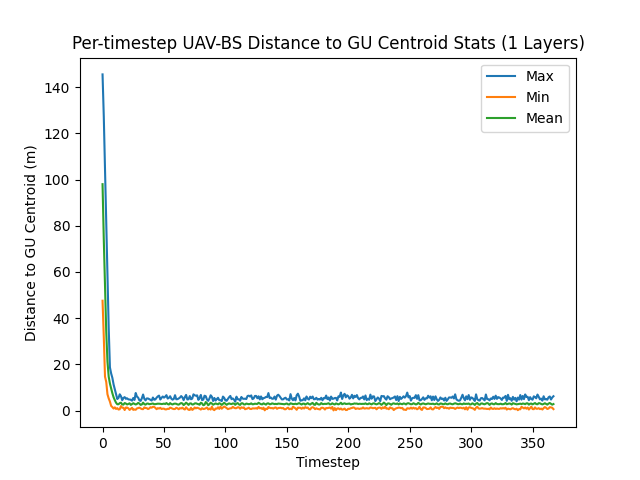
\includegraphics[width=0.43\textwidth]{figures/eve_test1/1_timestep_distance_to_centroid.png}
%       }
%       \hspace{1mm}
%    \subfigure[Maximum, Minimum \& Mean Distances to the \acrshort{lu} Centroid Across 30 Episodes]{\label{fig:ep_dist_to_centroid}
%           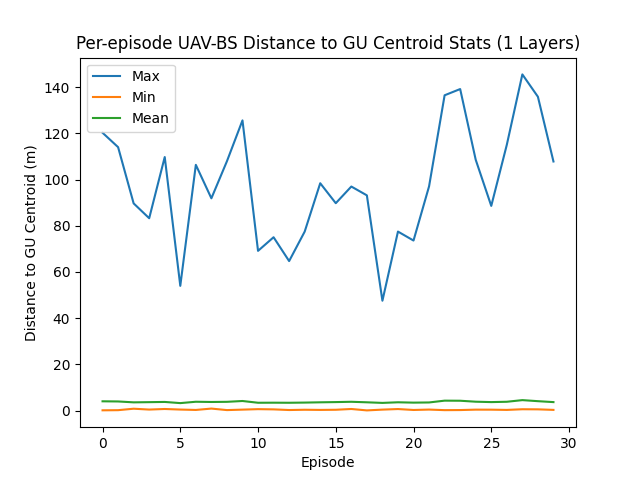
\includegraphics[height=0.21\textheight]{figures/eve_test1/1_episode_distance_to_centroid.png}
%       }
%       \caption{Proximity of the \acrshort{uav} to the \acrshort{lu} Centroid}
%       \label{fig:dist_to_centroid_plots}
%\end{figure}
\begin{figure} [ht!]
    \centering
    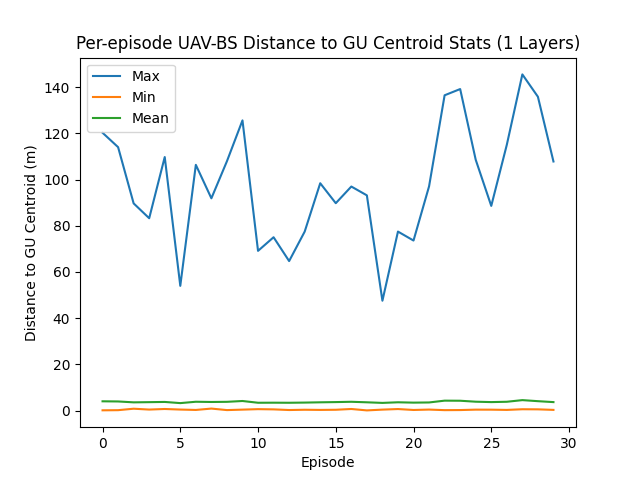
\includegraphics[width=0.75\linewidth]{figures/eve_test1/1_episode_distance_to_centroid.png}
    \caption{Maximum, Minimum \& Mean Distances to the \acrshort{lu} Centroid Across 30 Episodes}
    \label{fig:episode_dist_to_centroid}
\end{figure}
\begin{figure} [ht!]
    \centering
    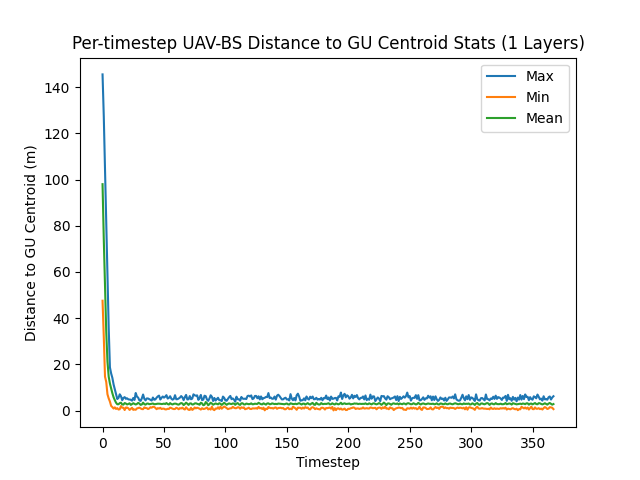
\includegraphics[width=0.75\linewidth]{figures/eve_test1/1_timestep_distance_to_centroid.png}
    \caption{Maximum, Minimum \& Mean Distances to \acrshort{lu} Centroid Per Timestep Across 30 Episodes}
    \label{fig:timestep_dist_to_centroid}
\end{figure}
As can be seen in Fig. \ref{fig:episode_dist_to_centroid} and Fig. \ref{fig:timestep_dist_to_centroid}, the \acrshort{uav} converged towards the \acrshort{lu} centroid (10 m above the average x, y co-ordinates for all \acrshort{lu}s) from a number of randomly generated starting locations where it was initialised in each episode. 
This demonstrates that the \acrshort{uav} consistently learned to achieve this objective, regardless of where it started in the simulation. 

\begin{figure} [ht!]
    \centering
    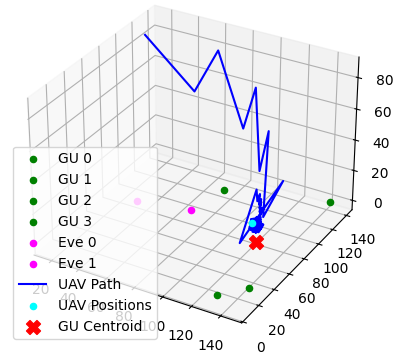
\includegraphics[width=0.75\linewidth]{figures/1_layers_uav_trajectory_20_timestep_370.png}
    \caption{\acrshort{uav} Trajectory in Simulated Environment}
    \label{fig:uav_trajectory_cube}
\end{figure}
As can be seen in Fig. \ref{fig:uav_trajectory_cube}, the \acrshort{uav} managed to learn, based on the observed state of the environment, to converge on the centroid of the \acrshort{lu}s despite its initial position being on the far side of the flight area. 
\subsection{Energy Efficiency}
The stabilisation and convergence of $\eta(t)$, i.e., the energy efficiency at timestep $t$ and $\eta (T)$, i.e., the integral of the energy efficiency from $t=0$ to $t=T$ is shown in Fig. \ref{fig:step_energy_eff} \& \ref{fig:ep_energy_eff}, respectively. 
A mean value of ~40kbps/Hz/J for $\eta(T)$ is maintained for all episodes in the simulation as the agent exhibits that it can and does effectively learn to optimise $\eta(t)$ early in the simulation with a single-layered ansatz in the actor and critic networks' quantum circuits. 
\begin{figure} [ht!]
    \centering
    %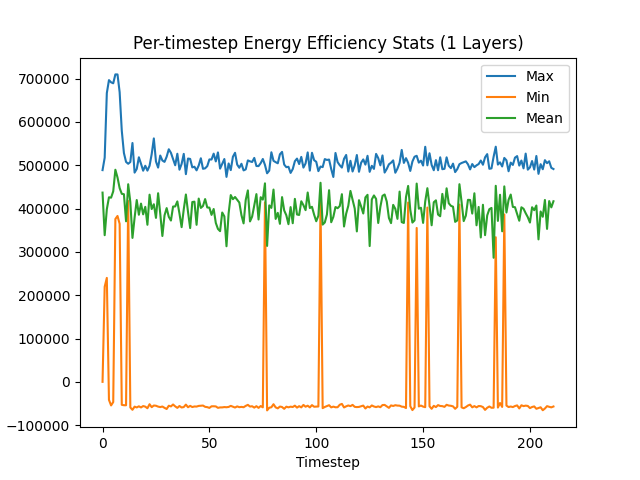
\includegraphics[width=0.75\linewidth]{figures/test9/1_timestep_energy_eff.png}
    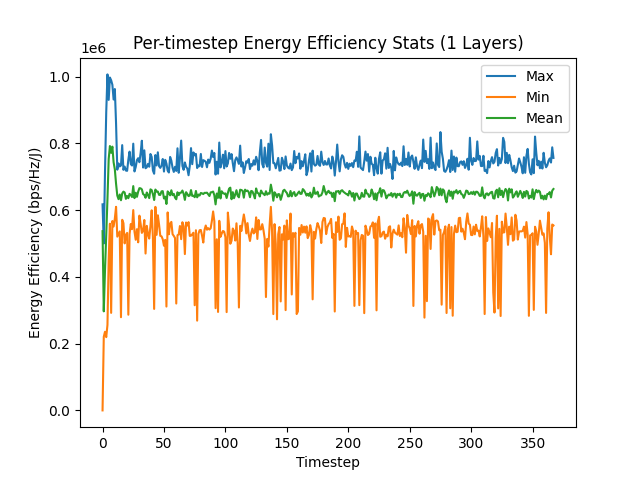
\includegraphics[width=0.75\linewidth]{figures/plots_eve_outputs/test3/1_timestep_energy_eff.png}
    \caption{Maximum, Minimum \& Mean Energy Efficiency Per Timestep}
    \label{fig:step_energy_eff}
\end{figure}

\begin{figure} [ht!]
    \centering
    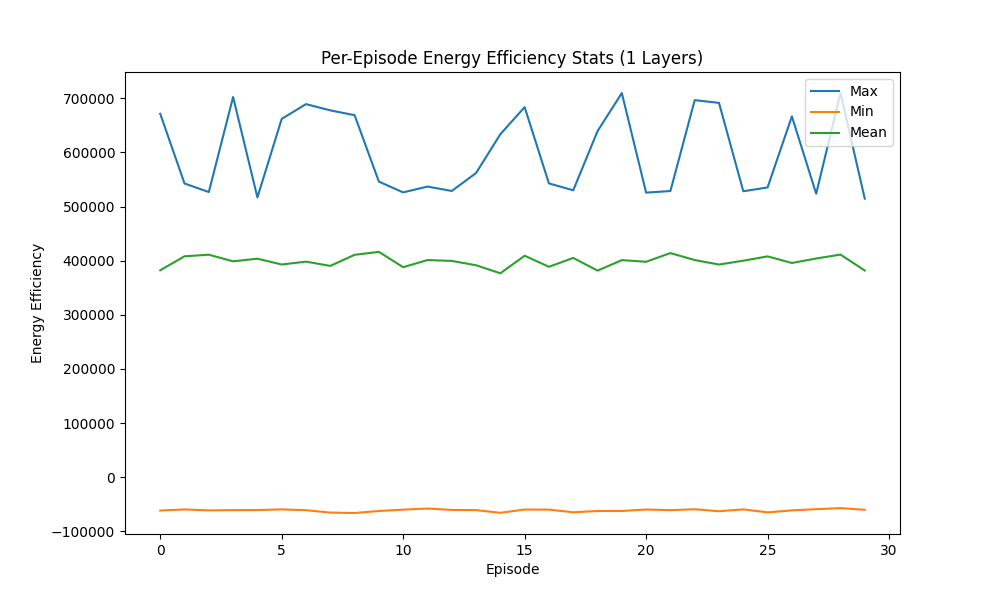
\includegraphics[width=0.75\linewidth]{figures/test9/1_episode_energy_eff.png}
    \caption{Energy Efficiency Across 30 Episodes}
    \label{fig:ep_energy_eff}
\end{figure}
As shown in Fig. \ref{fig:step_energy_eff} and Fig. \ref{fig:ep_energy_eff}, $\eta_{EE} (t)$ converges consistently towards \~ 40kbps/Hz/J across all of the 30 episodes that were run. 

As the \acrshort{uav} trajectory has been optimised as well as the data exchange rate and the secrecy rate, the energy efficiency increases as the \acrshort{uav} converges towards a lower level of energy consumption as it ceases to move around the environment and is able to hover above the optimal location for secure communications with the \acrshort{lu}s. 

%\begin{figure}[ht!]
%   \centering
%       \subfigure[Maximum, Minimum \& Mean Energy Efficiency Per Timestep]{\label{fig:step_energy_eff}
%           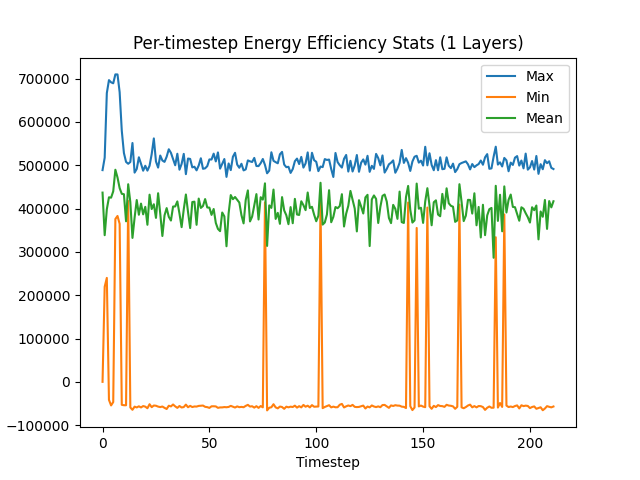
\includegraphics[width=0.42\textwidth]{figures/test9/1_timestep_energy_eff.png}
%       }
%       \hspace{1mm}
%    \subfigure[Energy Efficiency Across 30 Episodes]{\label{fig:ep_energy_eff}
%           %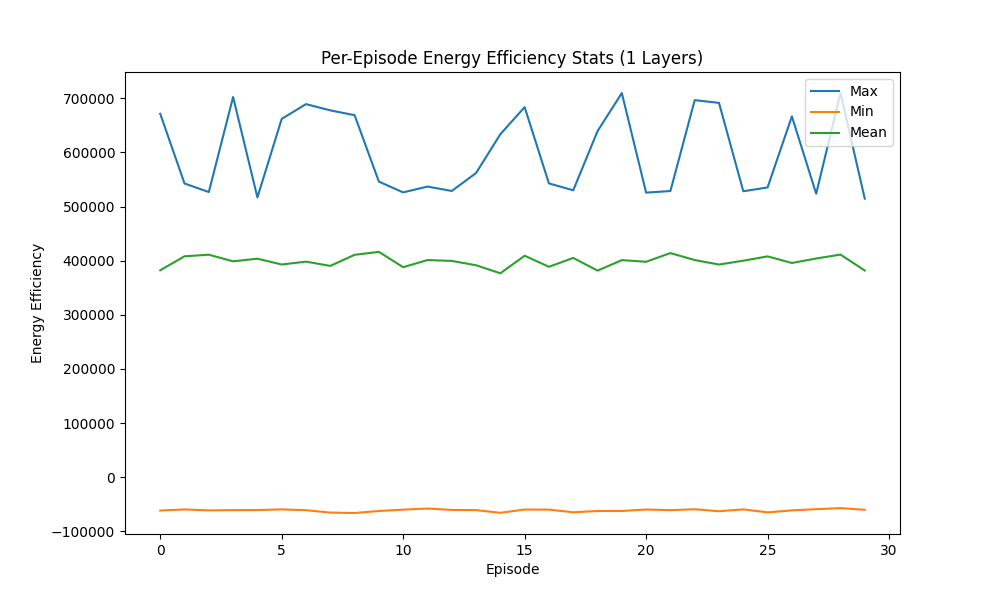
\includegraphics[width=0.45\textwidth]{figures/test9/1_episode_energy_eff.png}
%           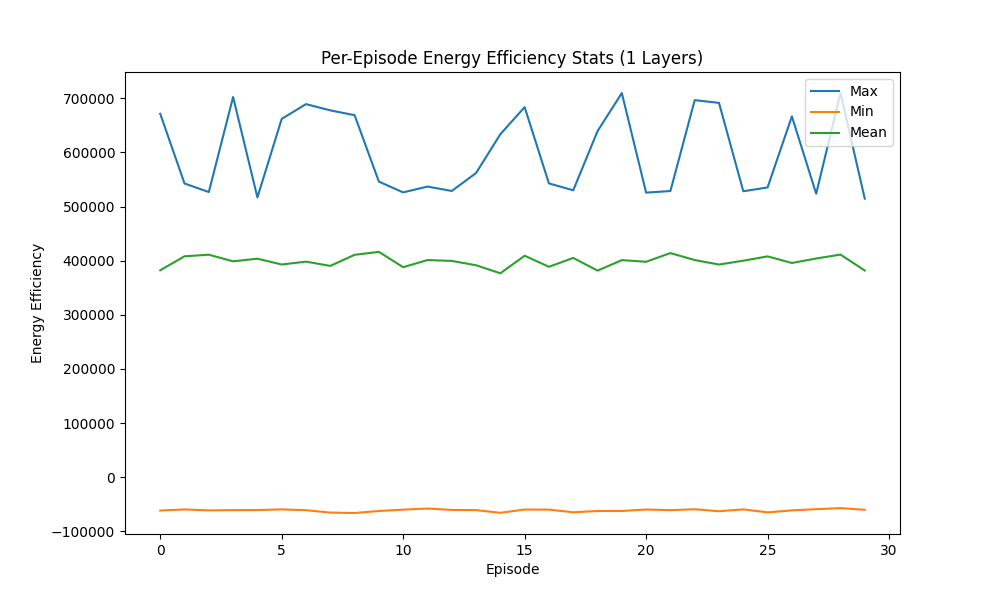
\includegraphics[height=0.2\textheight]{figures/test9/1_episode_energy_eff.png}
%       }
%       \caption{Energy Efficiency Data using a \acrshort{per}}
%       \label{fig:energy_eff_figs}
%\end{figure}
\subsection{Data Exchange Rate}
The data exchange rate $R_{U, k} (t)$ is used to shape the reward allocation along with penalties for violating the constraints of the joint optimisation problem. 
As rewards are dependent on the data exchange and secrecy rates for all \acrshort{lu}s and $\eta (t)$ is a function of $R_{U, k} (t)$, the maximisation of $\eta (T)$ requires that $R_{U, k} (t)$ is maximised and $E_{cons}$ is minimised.

\begin{figure} [ht!]
    \centering
    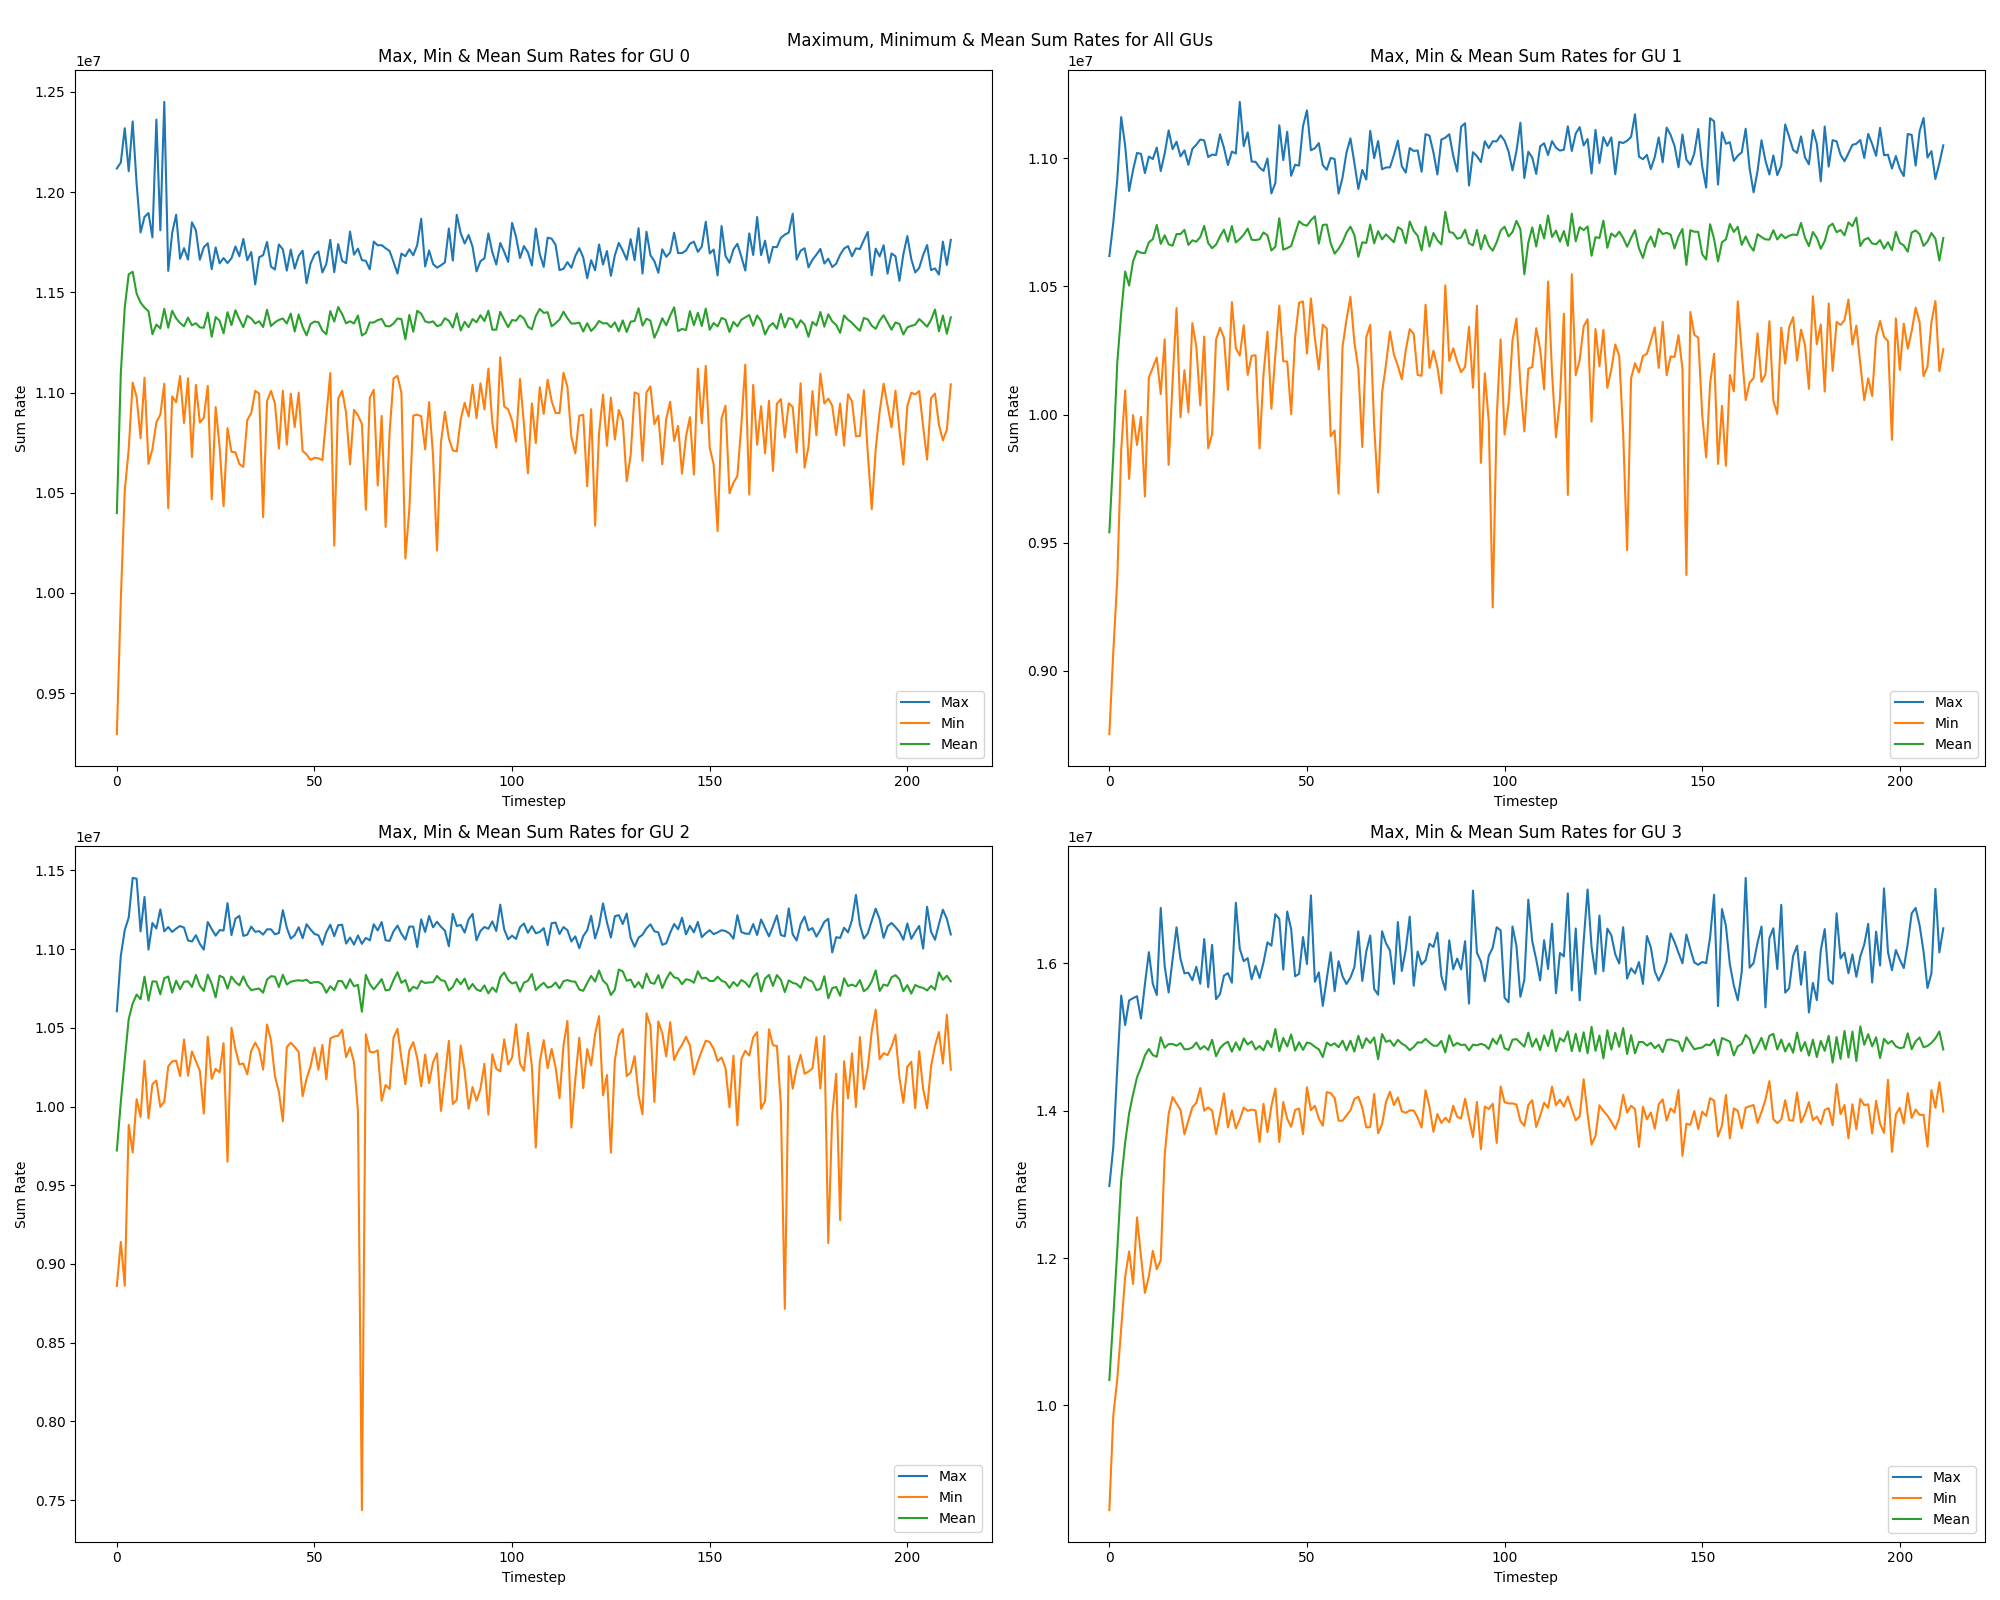
\includegraphics[width=0.9\textwidth]{figures/test9/fixed_1_timestep_sum_rate_all_GUs.png}
    \caption{Maximum, Minimum \& Mean $R_{U, k} (t)$ Values in Mbps from $t$ to $T$ Across 30 Episodes}
    \label{fig:timestep_sum_rates_all_gus}
\end{figure}
As shown in Fig. \ref{fig:timestep_sum_rates_all_gus}, for all of the legitimate \acrshort{gu}s in the simulated scenario, the average sum rate converges from $0$ to above 10 Mbps for $R_{min} = 9.5\ Mbps$ consistently within a short period of time. 

Fig. \ref{fig:episodes_sum_rates_all_gus} displays the maximum, minimum and mean values for the data exchange rates across 30 episodes. 
Again, it can be seen that the agent effectively managed to learn to maximise $R_{U, k} (t)$ for all \acrshort{lu}s such that the $R_{min}$ threshold has been met for all \acrshort{lu}s, ensuring fairness in the distribution of $R_{U, k} (t)$ for all $\mathcal{K}$ \acrshort{lu}s. 
\begin{figure} [ht!]
    \centering
    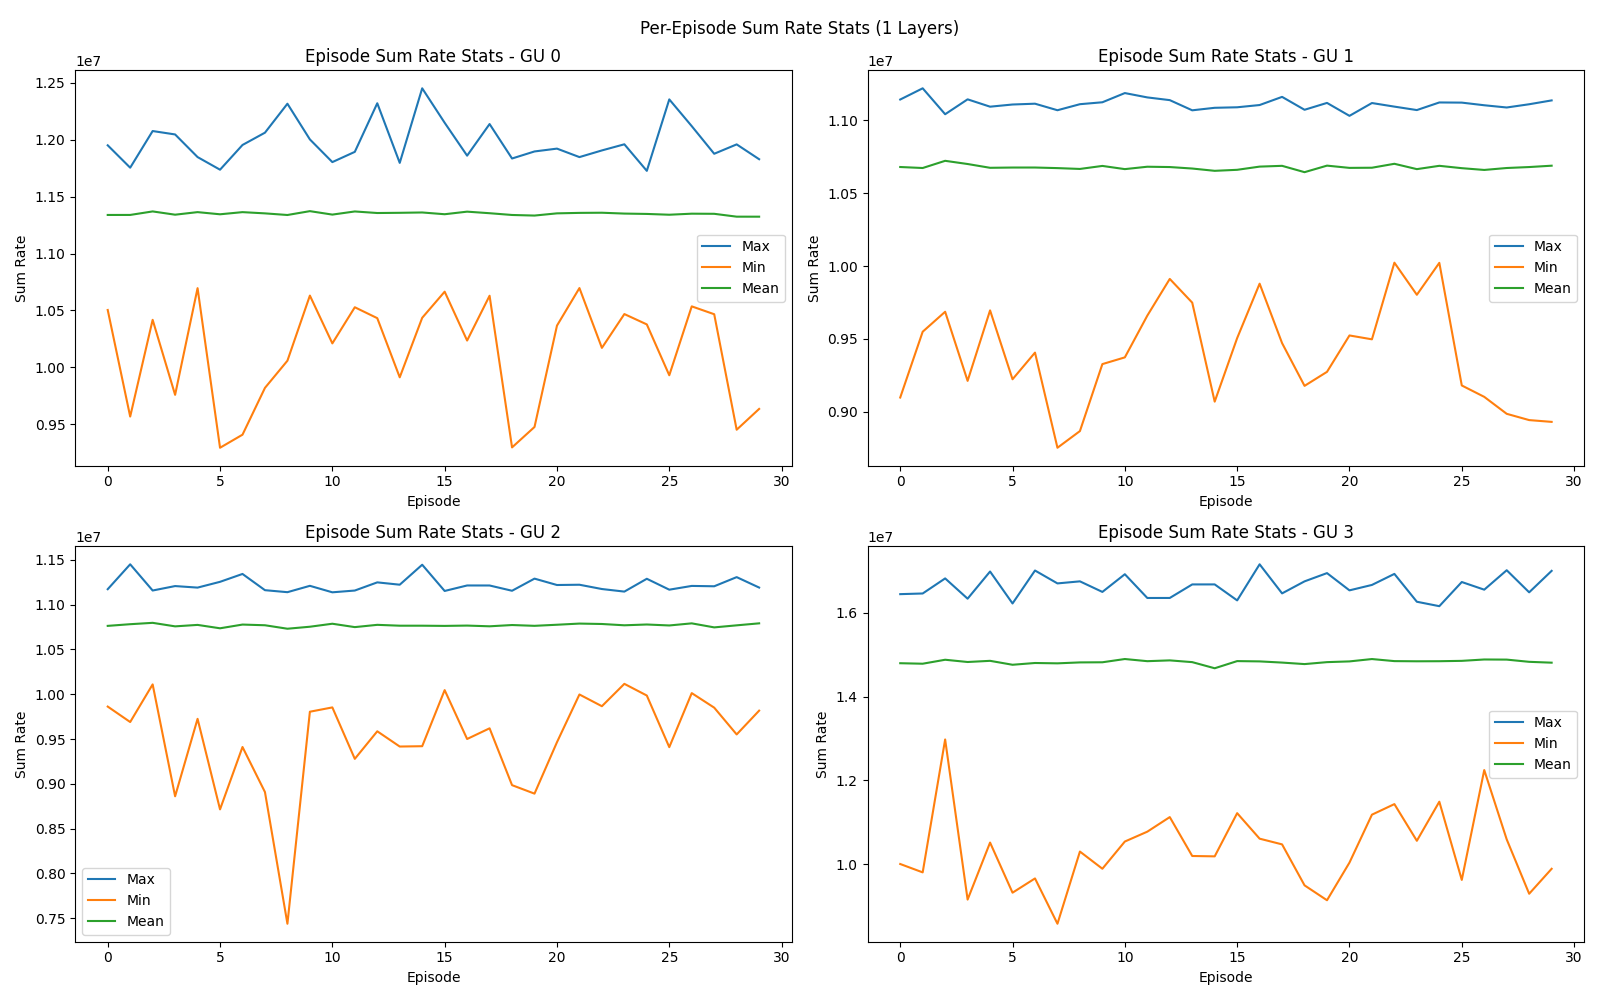
\includegraphics[width=0.9\textwidth]{figures/test9/1_episode_sum_rate_stats.png}
    \caption{Maximum, Minimum \& Mean $R_{U, k} (t)$ in Mbps Values Across 30 Episodes}
    \label{fig:episodes_sum_rates_all_gus}
\end{figure}

This demonstrates that the agent effectively learns to maximise the data exchange rate as well as the fairness in data rates for all \acrshort{gu}s such that all \acrshort{gu}s receive an acceptable and consistent \acrshort{qos}. 
None of the \acrshort{lu}s have a value for $R_{U, k} (t) < R_{min}$ upon convergence, thus adhering to the constraints of the optimisation of $R_{U, k} (t)$. 

%\begin{figure}[ht!]
%    \centering
%    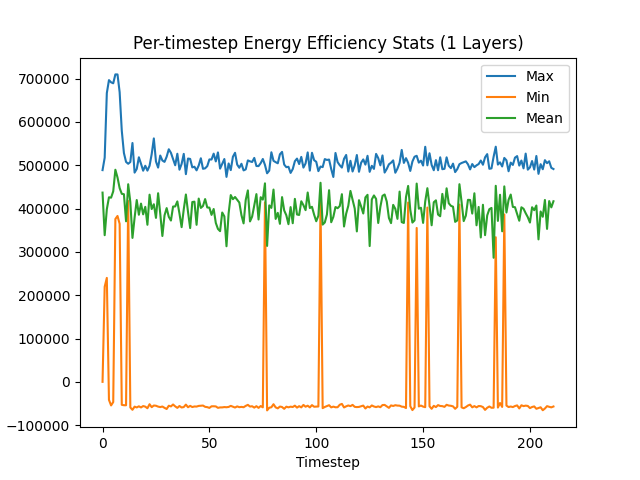
\includegraphics[width=0.5\linewidth]{figures/test9/1_timestep_energy_eff.png}
%    \caption{Caption}
%    \label{fig:step_energy_eff}
%\end{figure}
%
%\begin{figure}[ht!]
%    \centering
%    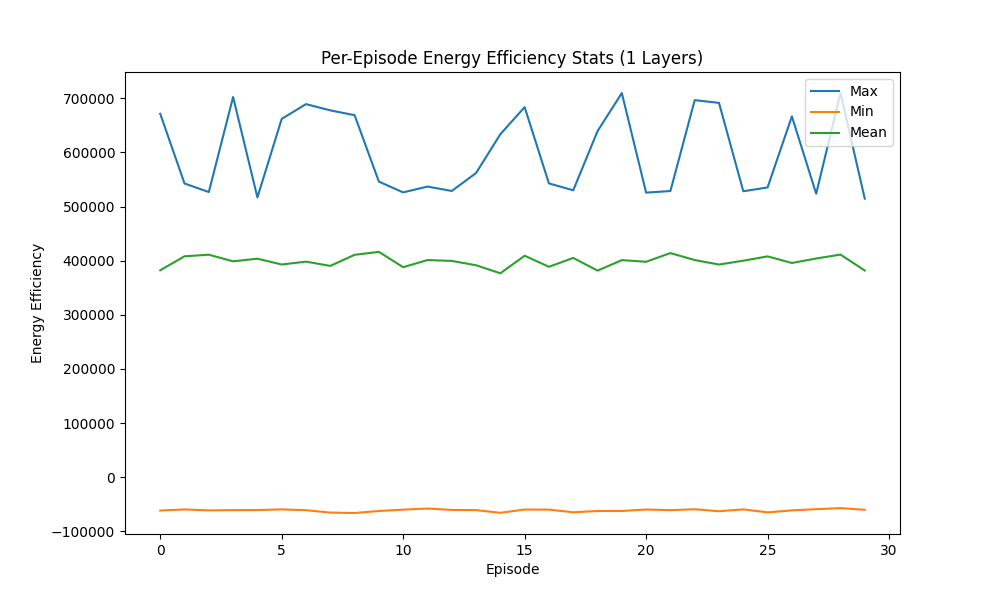
\includegraphics[width=0.5\linewidth]{figures/test9/1_episode_energy_eff.png}
%    \caption{Caption}
%    \label{fig:ep_energy_eff}
%\end{figure}
%\subsection{Data Exchange Rate}

\subsection{Secrecy Rate}
The secrecy rate for the \acrshort{uav}-\acrshort{lu} communications had to be above $R_{min}^{sec} = R_{min} = 9.5\ Mbps$. 
This was achieved with a single layer in the actor-critic quantum circuits and is shown in Fig. \ref{fig:timestep_secrecy_rate_all_gus} and Fig. \ref{fig:episode_secrecy_rate}, respectively. 

\begin{figure} [ht!]
    \centering
    %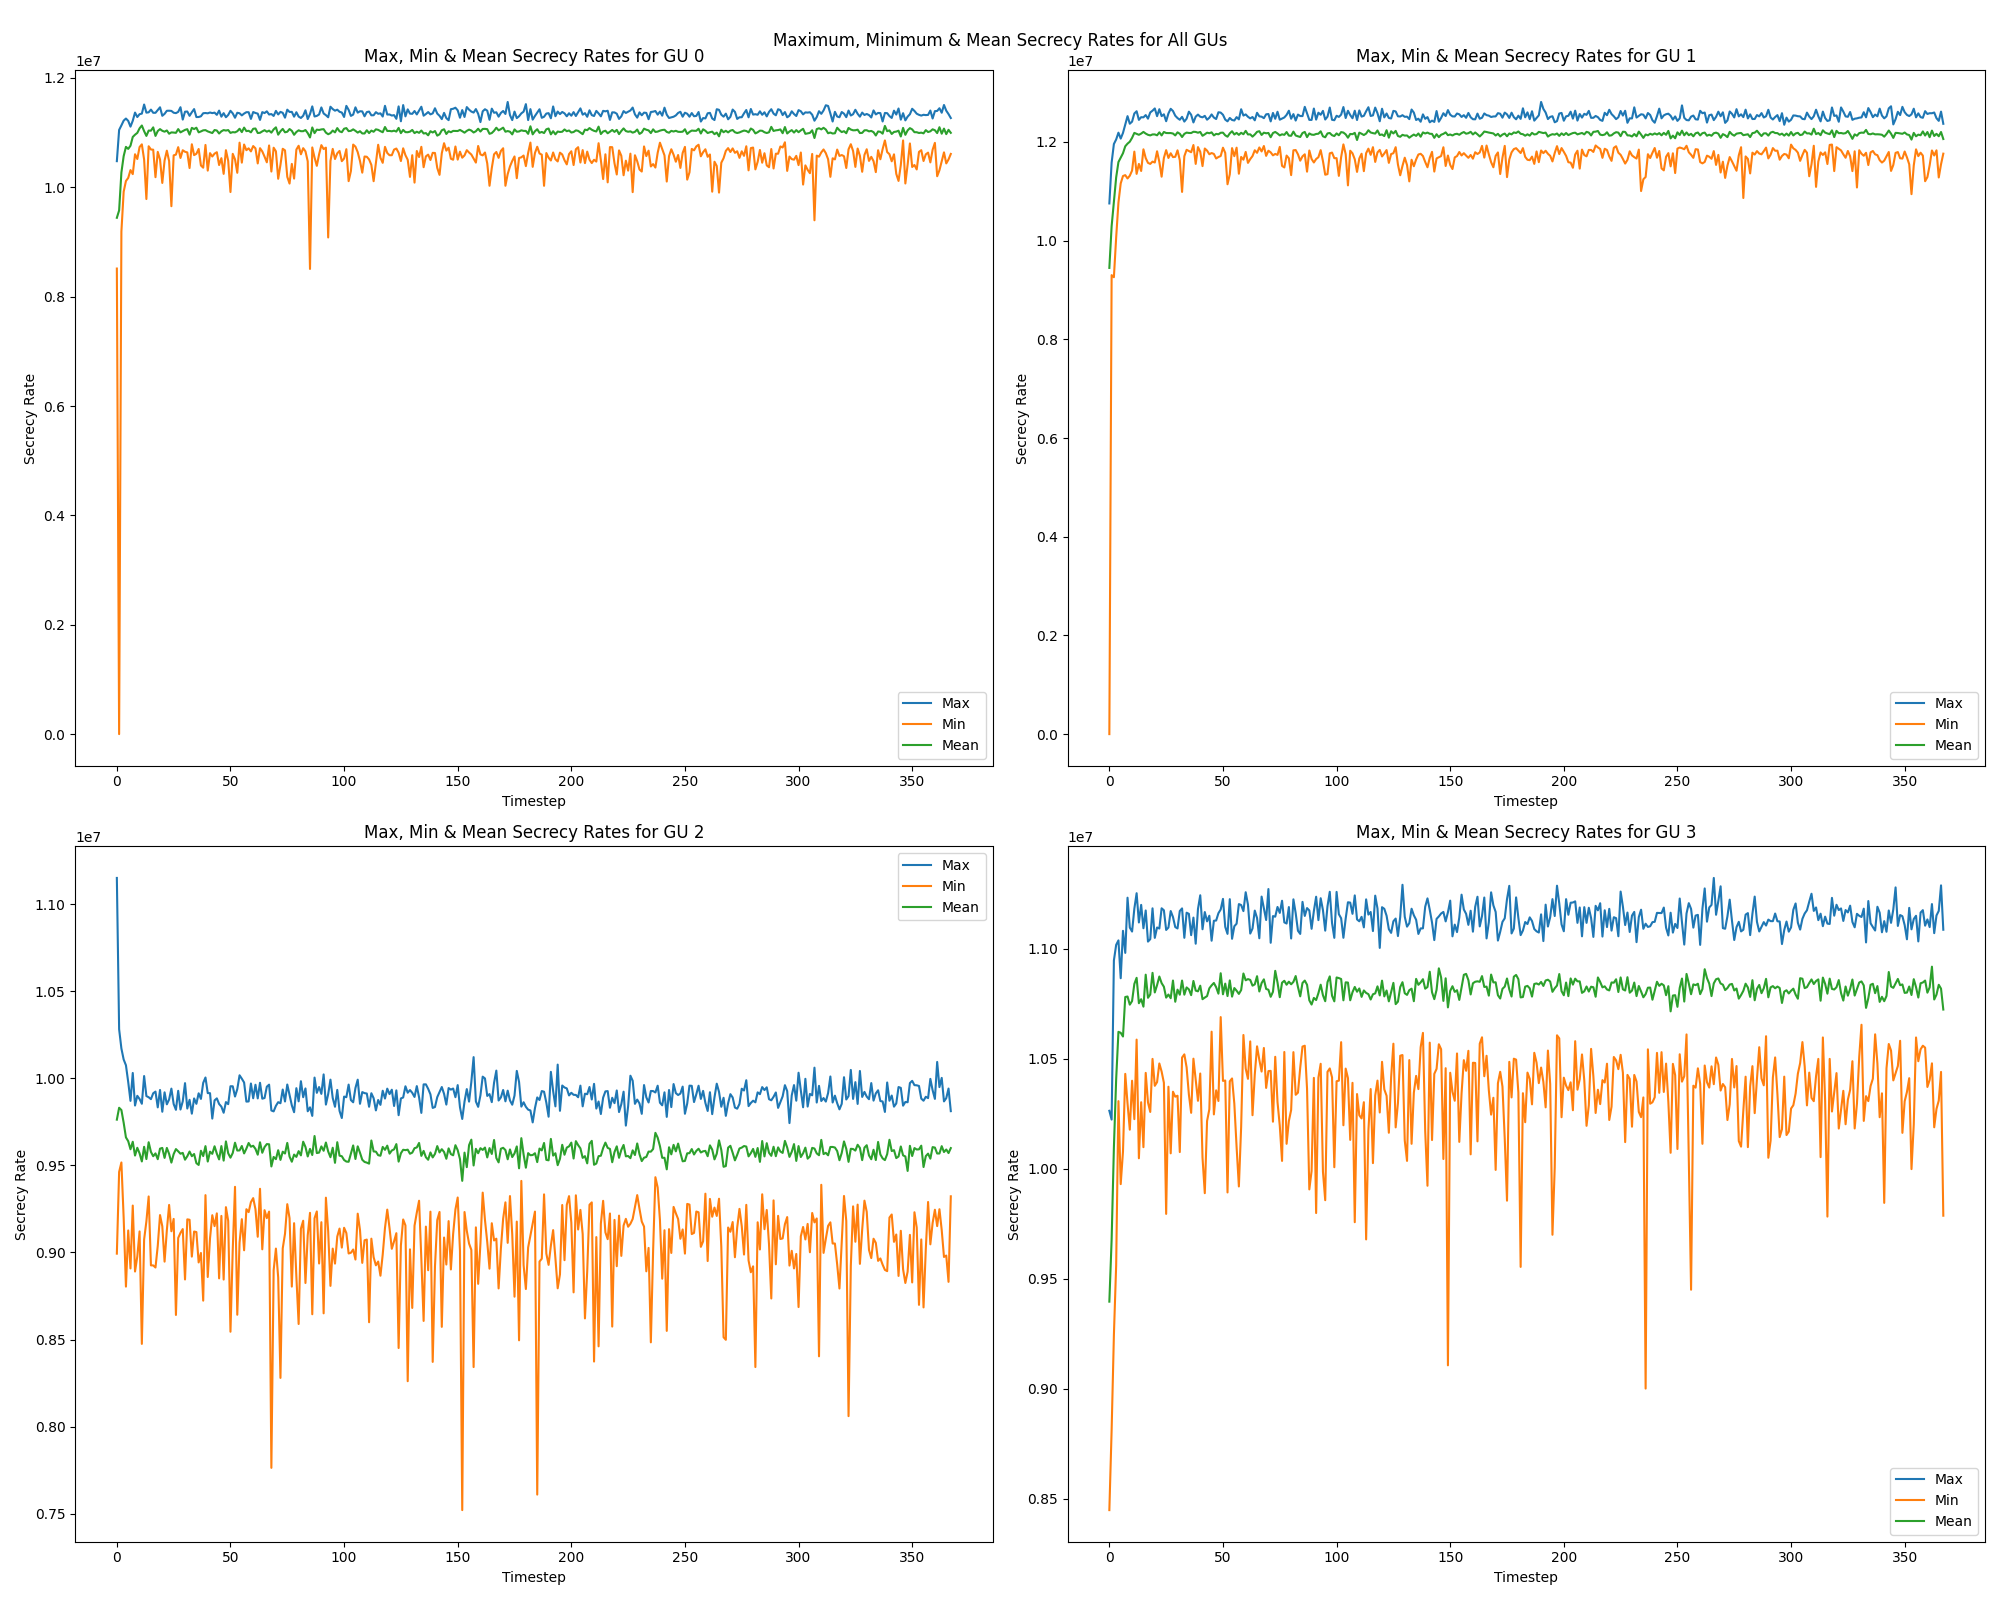
\includegraphics[width=1\textwidth]{figures/eve_test1/1_timestep_secrecy_rate_all_GUs.png}
    %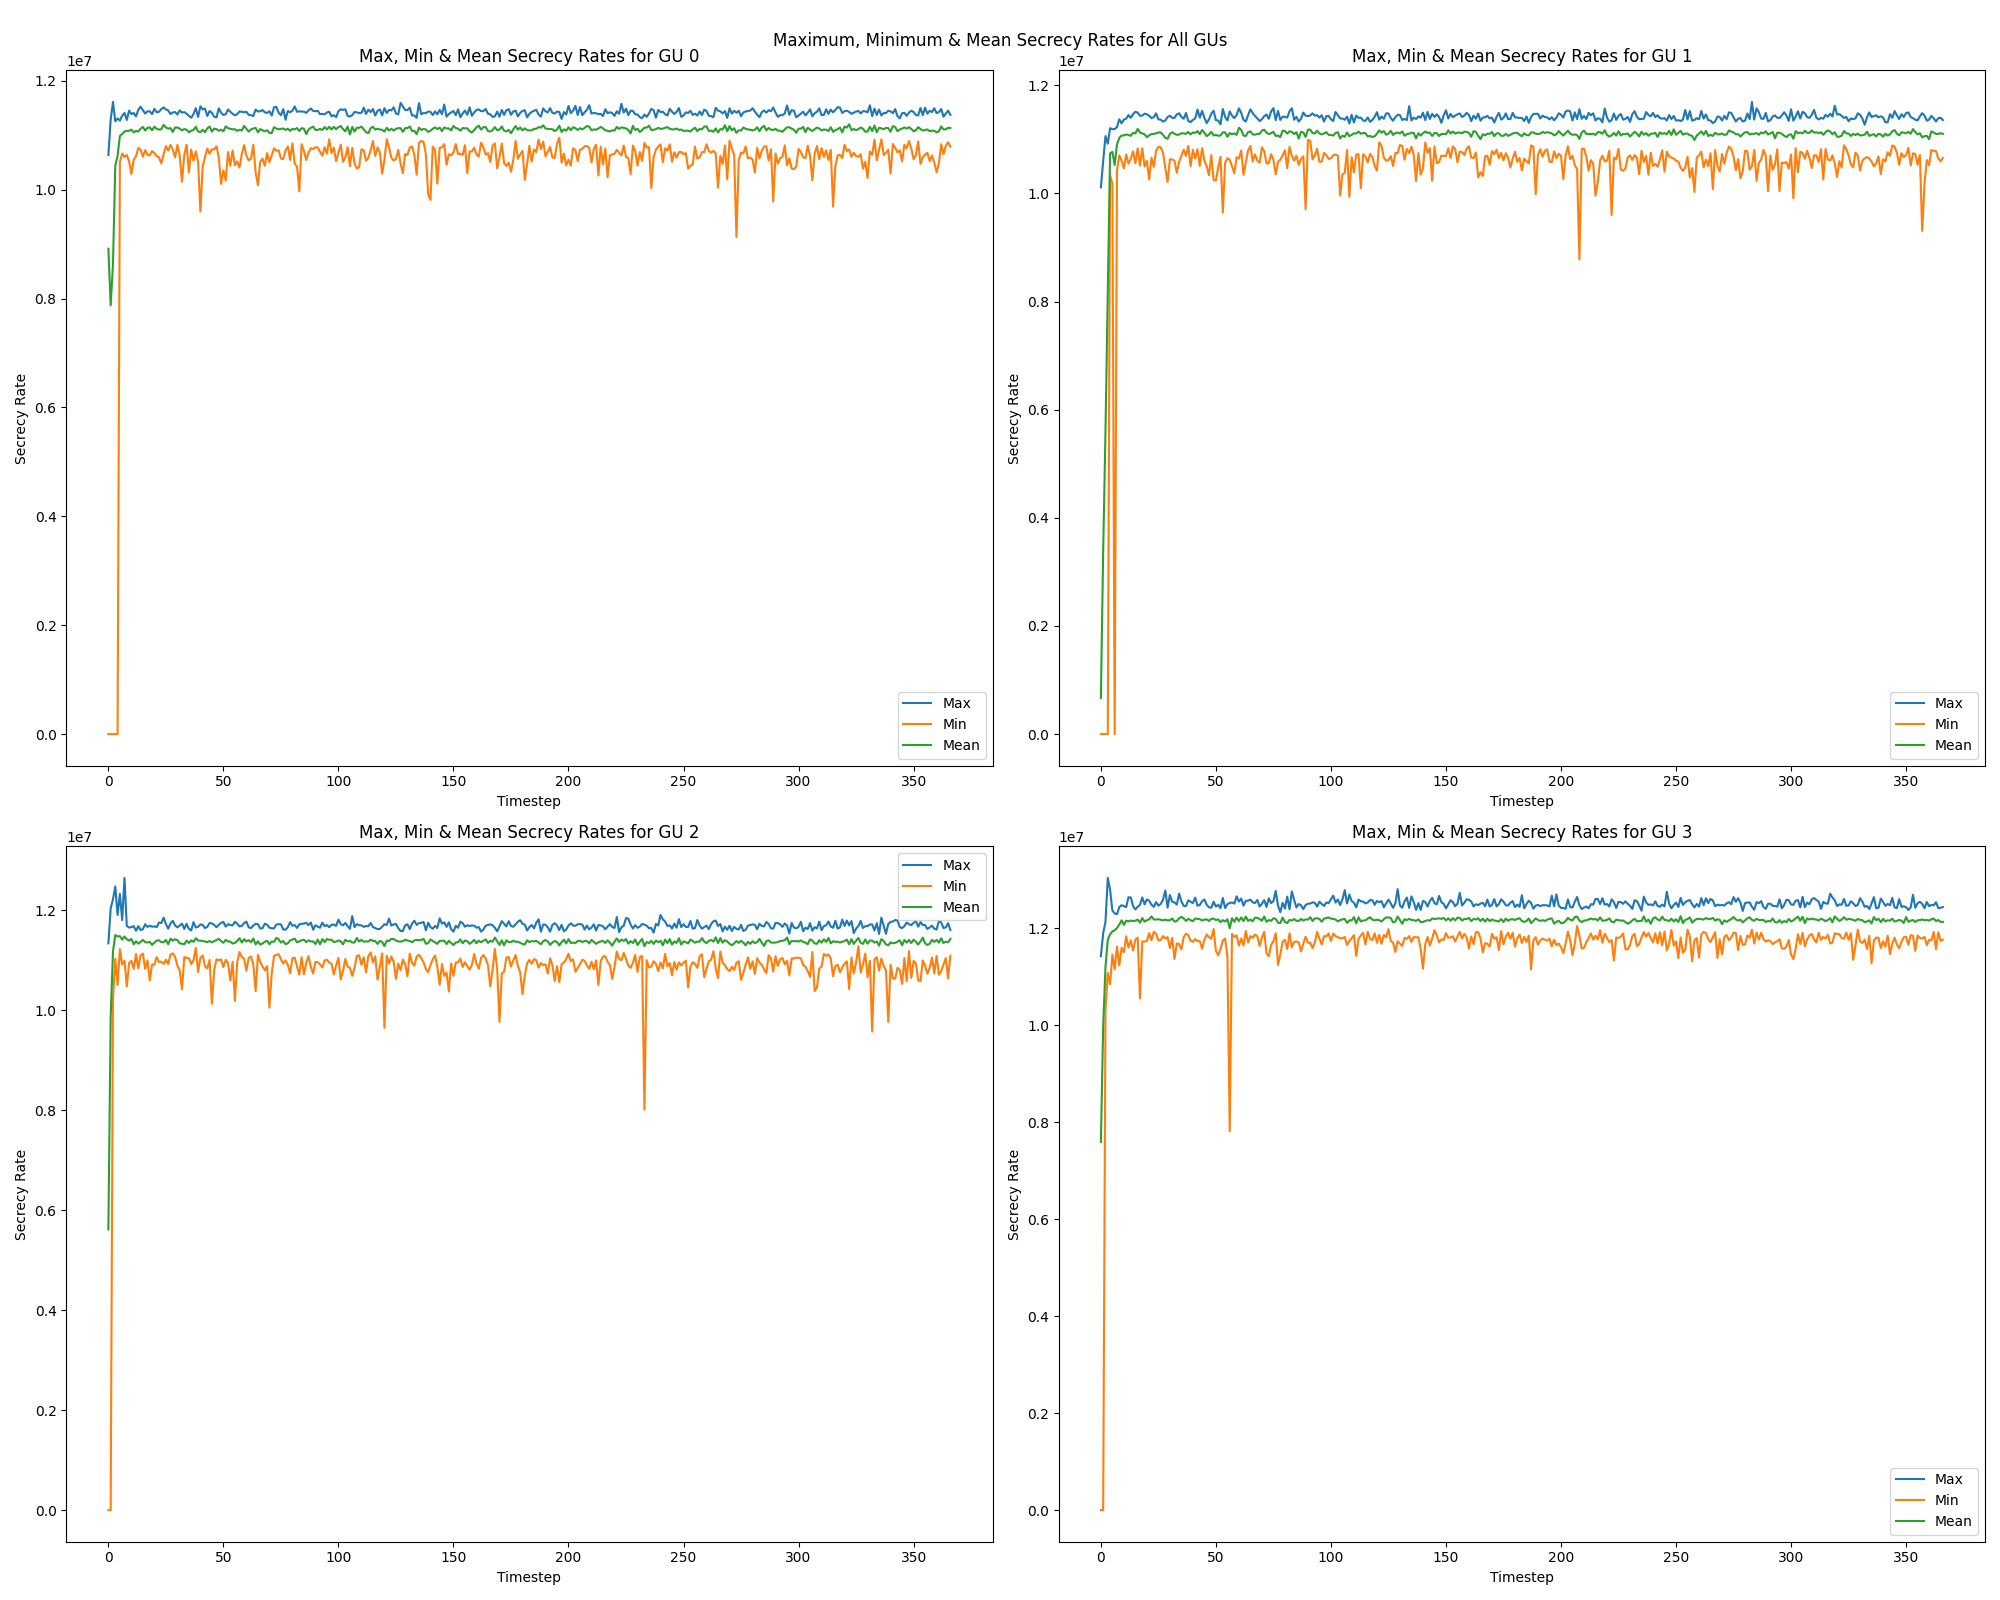
\includegraphics[width=1\textwidth]{figures/eve_out/1_timestep_secrecy_rate_all_GUs.png}
    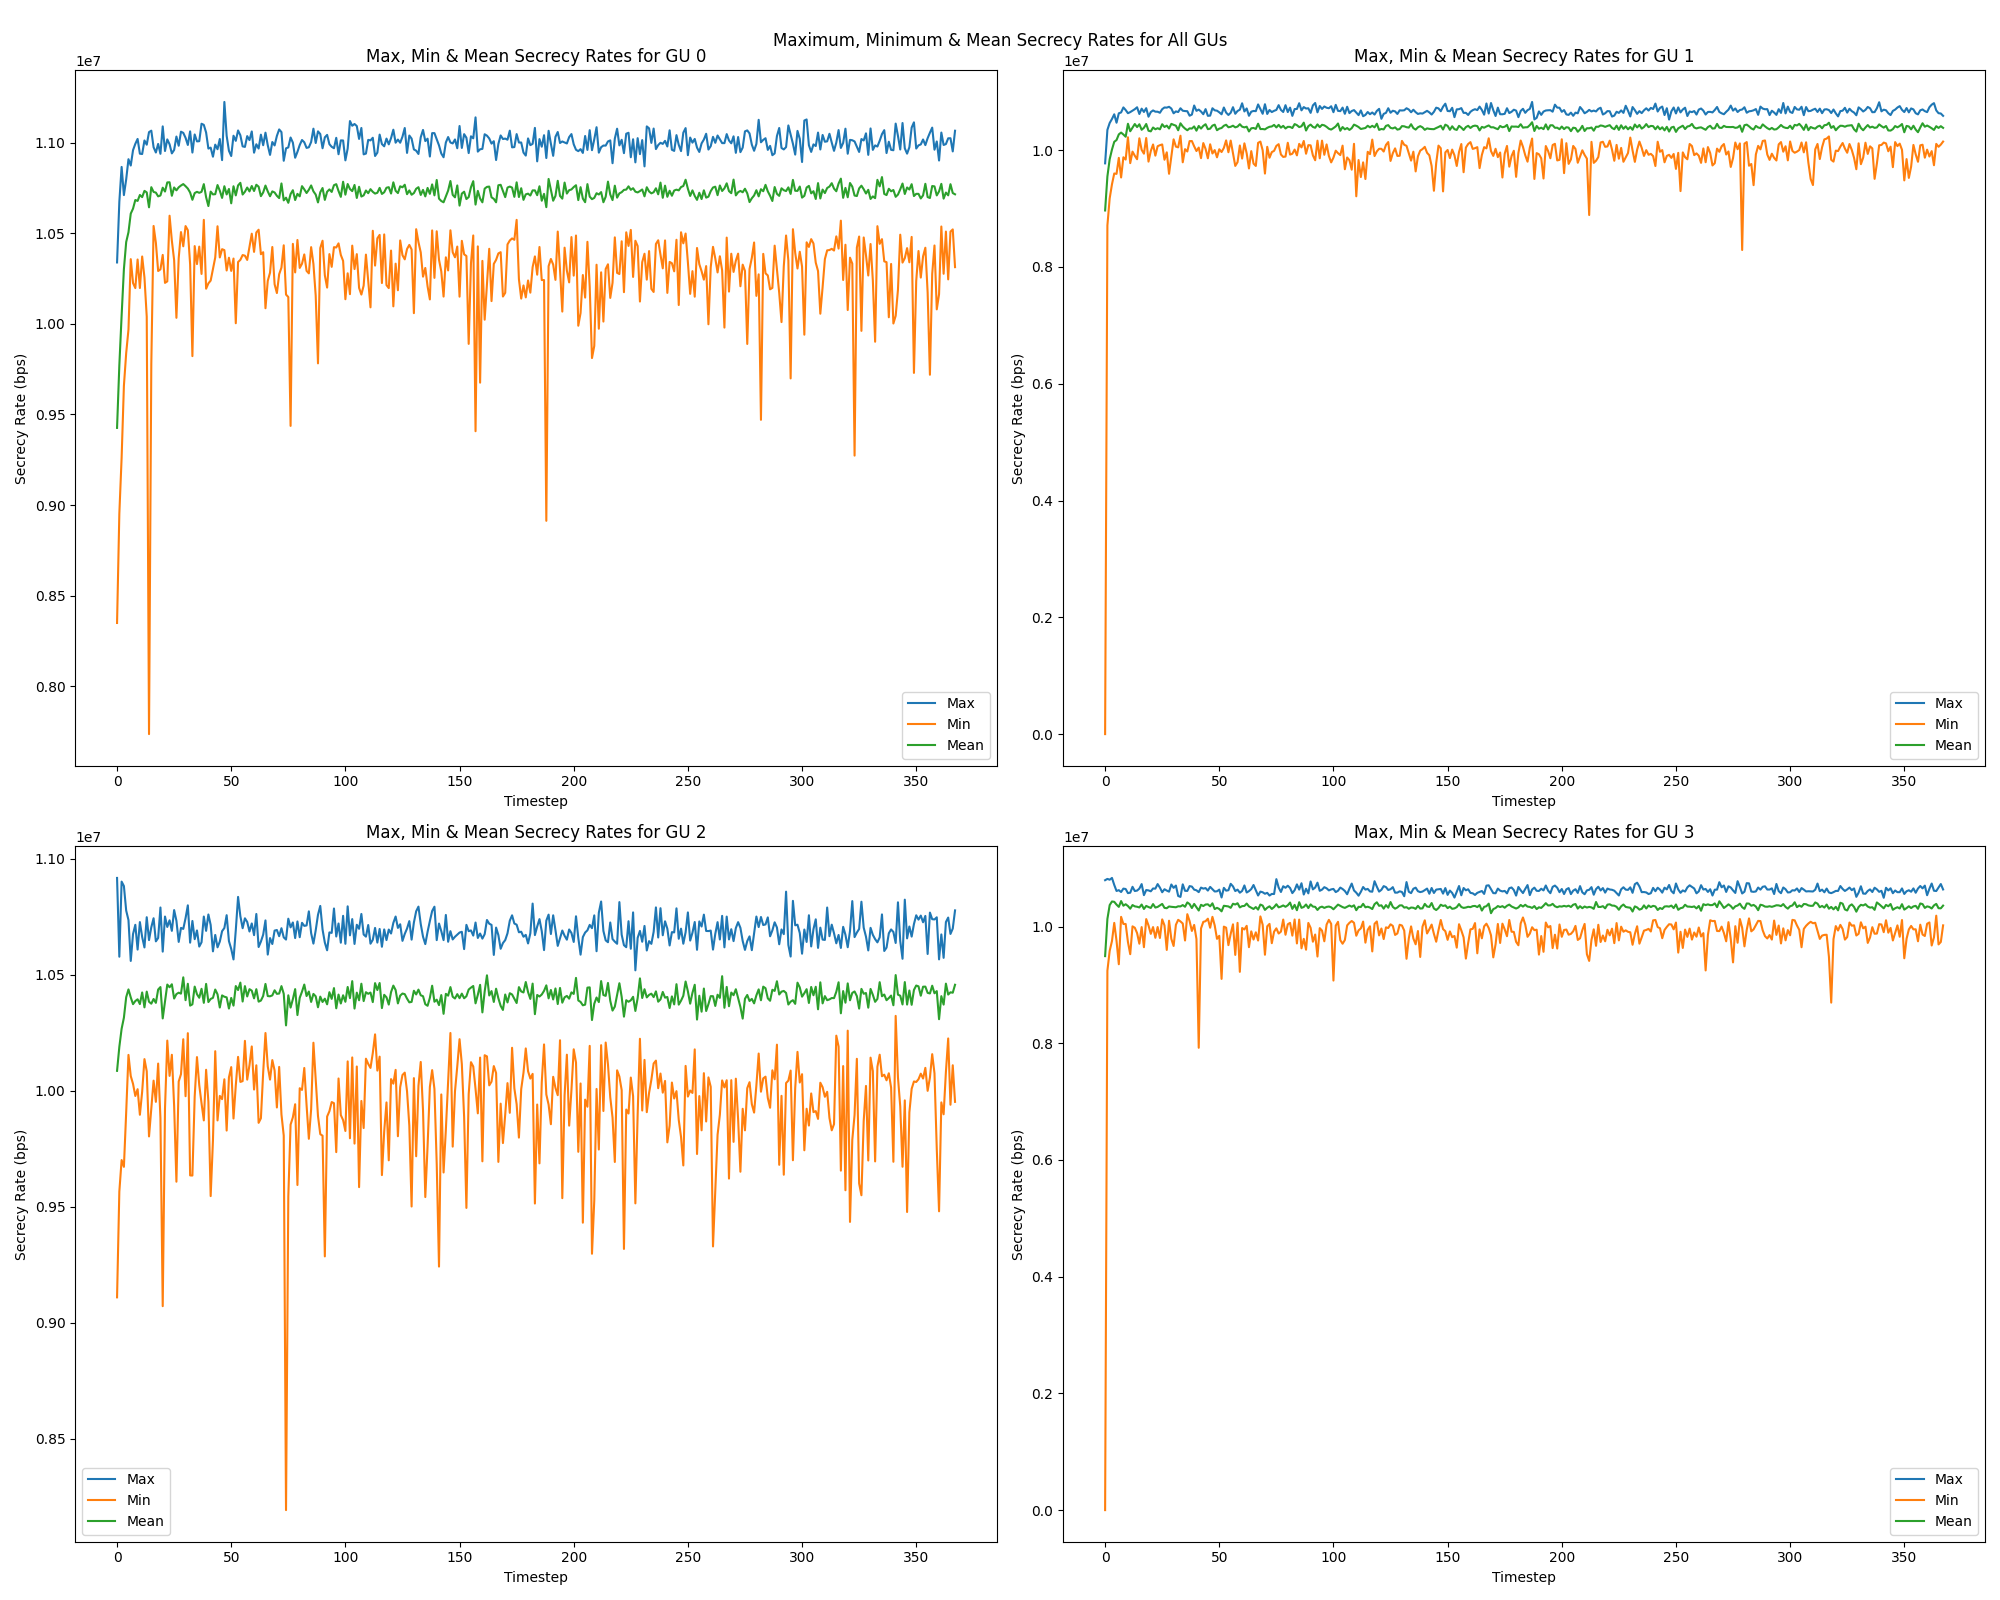
\includegraphics[width=0.9\textwidth]{figures/plots_eve_outputs/test3/1_timestep_secrecy_rate_all_GUs.png}
    \caption{Maximum, Minimum \& Mean Secrecy Rates for all \acrshort{lu}s for each Timestep Across 30 Episodes}
    \label{fig:timestep_secrecy_rate_all_gus}
\end{figure}

\begin{figure} [ht!]
    \centering
    %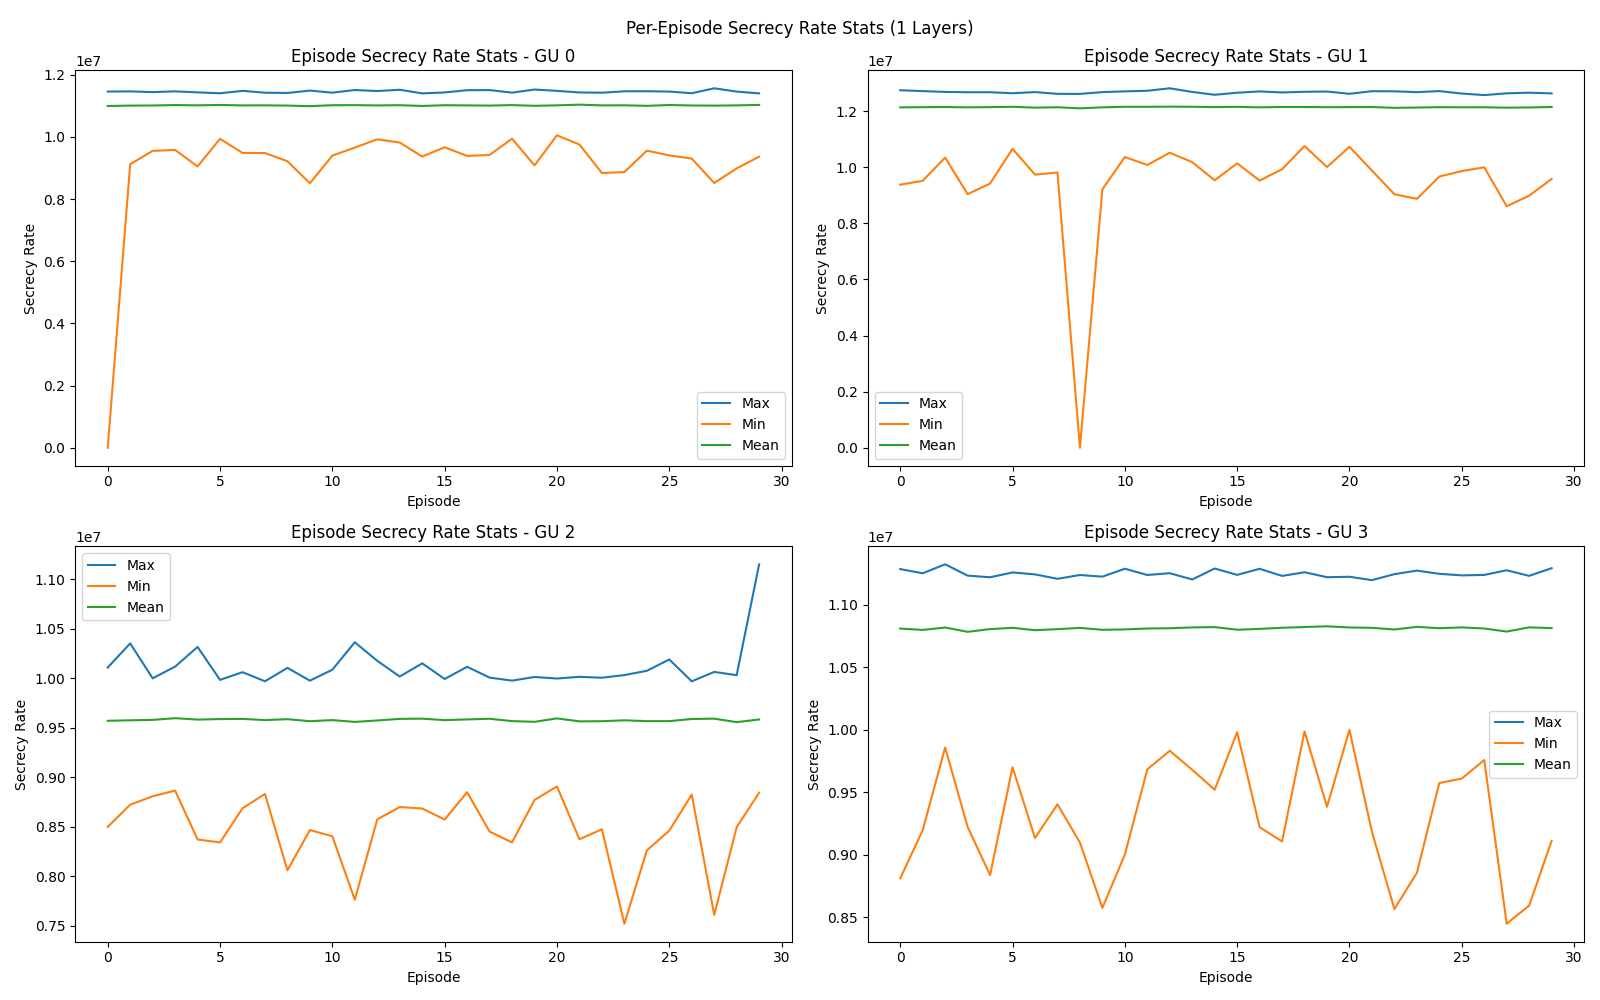
\includegraphics[width=1\textwidth]{figures/eve_test1/1_episode_secrecy_rate_stats.png}
    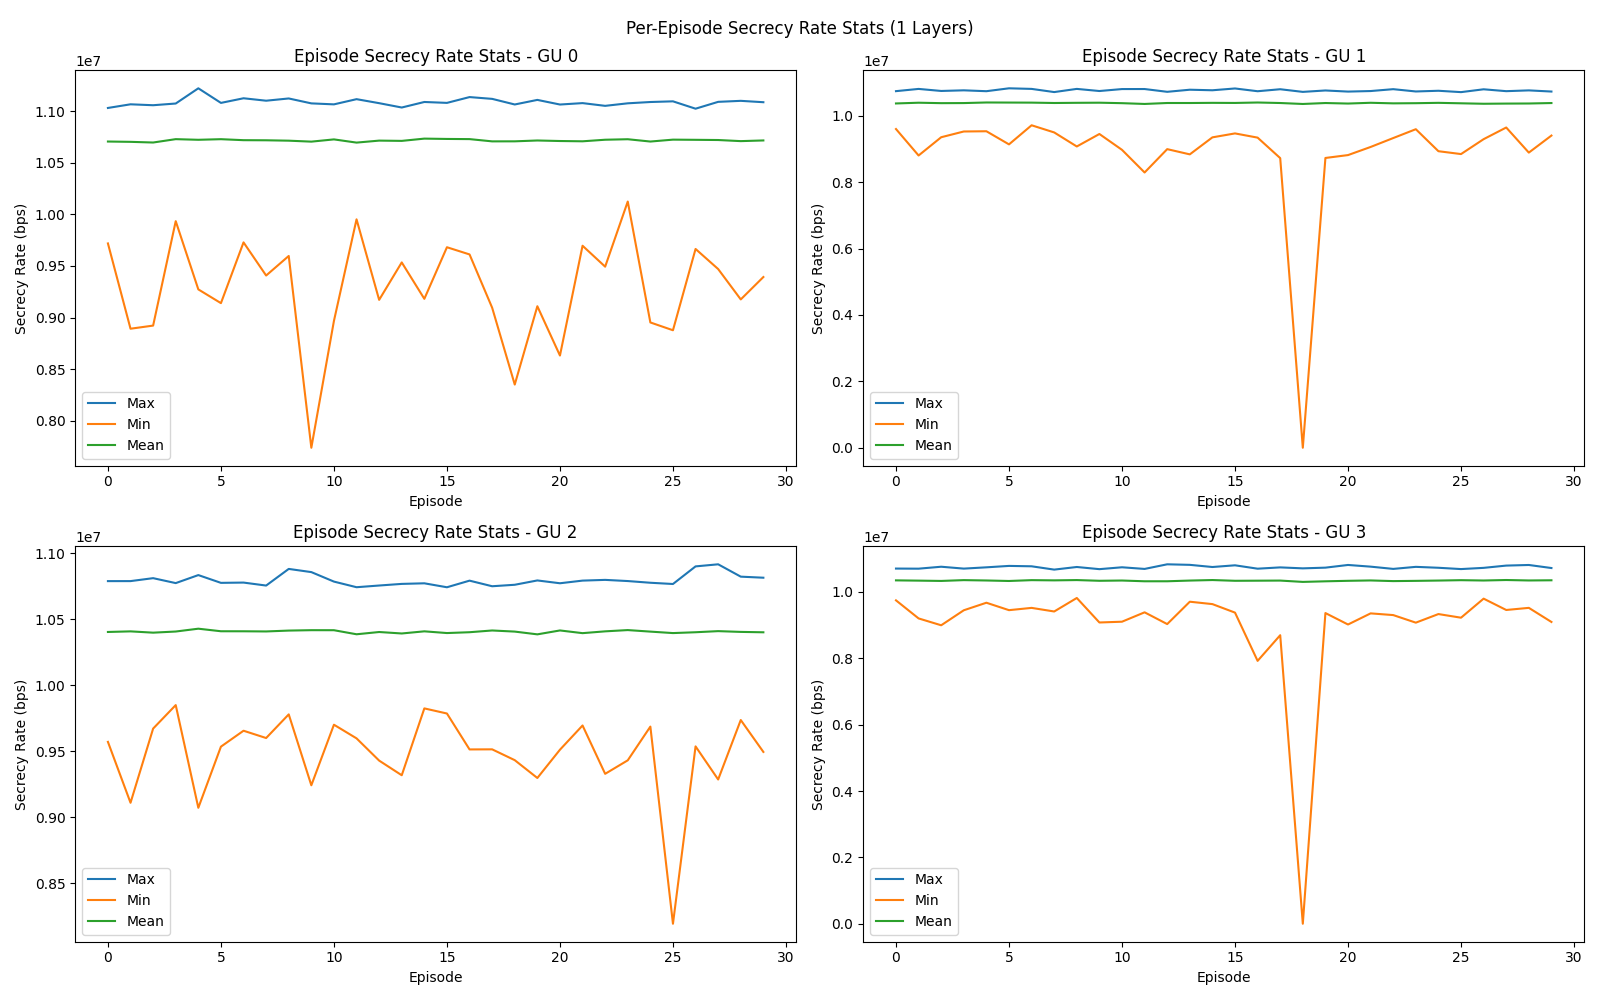
\includegraphics[width=0.9\textwidth]{figures/plots_eve_outputs/test3/1_episode_secrecy_rate_stats.png}
    \caption{Maximum, Minimum \& Mean Secrecy Rates for all \acrshort{lu}s Across 30 Episodes}
    \label{fig:episode_secrecy_rate}
\end{figure}

It can be seen that $R_{U, k}^{sec}$ converges to above $R_{min}^{sec}$ consistently, which is in-line with the increase in $R_{U, k}$, as the increase in $R_{U, k}^{sec}$ is dependent on the increase of $R_{U, k}$.
As shown in Fig. \ref{fig:timestep_secrecy_rate_all_gus} and Fig. \ref{fig:episode_secrecy_rate}, the threshold for the minimum acceptable secrecy rate was reached for all of the legitimate \acrshort{gu}s. 
No single \acrshort{lu} was left for it's average total secrecy rate $\bar{R}_{U, k}^{sec}$ to fall below $R_{min}^{sec}$. 

Each \acrshort{lu} had its secrecy rate converge to above 10 Mbps within the simulation to the point of the secrecy rate converging onto the value of the data exchange rate. 
This is a desirable outcome for this problem, demonstrating the efficacy of spiking the \acrshort{uav}-\acrshort{lu} communications with an \acrshort{ans}. 
This demonstrates that the Eve links were so affected by the \acrshort{ans} that their \acrshort{snr} plummeted to a very low value, i.e., any form of useful information from the signal was overpowered entirely by the \acrshort{ans}. 
This shows that the eavesdropping rate has dropped, increasing the secrecy rate and minimised the capabilities for Eves to conduct \acrshort{mitm} attacks on the \acrshort{lu}s. 
\section{\texorpdfstring{\acrshort{drl}}{DRL} Performance}
%\hl{DETAIL \& PLOT DRL ALGORITHM PERFORMANCE WITH DRL METRICS}
\subsection{Local Loss}
The critic loss within the algorithm began to decrease and stabilise around a small set of values for a single layer, as shown in \ref{fig:single_layer_critic_loss}. 

\begin{figure}[ht!]
    \centering
    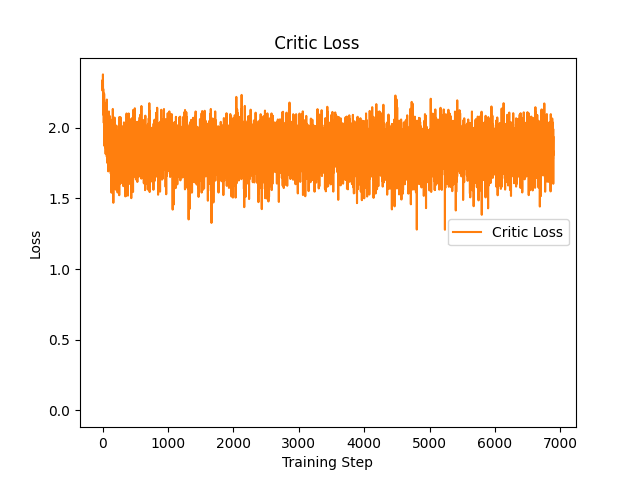
\includegraphics[width=0.75\linewidth]{figures/test9/1_layers_losses.png}
    \caption{Critic Loss for M = 1}
    \label{fig:single_layer_critic_loss}
\end{figure}
The results for the loss function from the critic network are quite noisy as a result of having to sampling and decode the values $K_{shot}$ times in a simulated open quantum system. 
The length of the quantum circuit is also quite large, with 17 inputs being fed into the critic network, leading to a noisy output prior to decoding, however, this did not appear to impact the results presented in the previous section in a negative way. 
\section{Quantum Actor-Critic Network}
The actor-critic network quantum circuitry appeared to perform most optimally with a single layer within the ansatz rather than increasing the number of layers. 

The quantum actor-critic network was tested with 1-5 layers within the system. 
This was performed to determine the impact on the number of layers and if the increase in the number of layers positively or negatively impacted the performance of the system beyond a particular number of layers. 

\subsection{Impact of the Number of Layers on Performance}
It was found that for higher numbers of layers beyond a single layer within the ansatz that the performance of the \acrshort{lqdrl} algorithm began to degrade and become far more unpredictable, leading to very noisy curves for the \acrshort{uav} trajectory, $\eta_{EE} (t)$, $R_{U, k}$ and $R_{U, k}^{sec}$. 

After 3 layers within the actor-critic ansatz circuits, it was observed that the results for the secrecy rate, data exchange rate, trajectory and energy efficiency all became far too noisy and unpredictable to be of any practical value. 

This phenomenon may arise from the fact that the same values are being recomputed repeatedly despite only a single layer being useful, leading to increased levels of noise arising from the increased depth of the quantum circuits. 

Figures with data for each timestep of each episode for each number of layers can be found in \ref{appendix_layers_figures}. 

As shown in \ref{appendix_layers_figures}, the results are consistent and converge towards their optimal values for the \acrshort{uav} trajectory and the data exchange rate, however, for increasing numbers of layers, the \acrshort{uav} can either do the opposite of what its objective is for M = 2 and begins to become too noisy and unpredictable for 3-5 layers. 
In the case of M = 2, the fact that the data exchange rate and the distance between the \acrshort{uav}-\acrshort{bs} and the \acrshort{lu} centroid converged to the opposite of the desired outcome could be useful for providing some insights into the optimisation problem, e.g., it could serve as a means to model a dual optimisation problem, however, this has not been explored extensively as part of this thesis. 
%\chapter{Discussion}
%
%\hl{Discuss errors?}
%
%\hl{(Farrell discussion: 2 pages)
%
%(Collins discussion: 0 pages)
%
%(Dunne discussion: 0 pages)}
\chapter{Conclusions}
\section{Achieved Objectives}
The core objective of the joint optimisation problem outlined in this thesis was to maximise the secrecy rate of \acrshort{uav}-\acrshort{lu} communications by optimising the \acrshort{uav} trajectory, data exchange rate and energy efficiency. 
The trajectory was minimised and the energy efficiency, data exchange rates and secrecy rates were all maximised and shown to converge consistently across a range 30 of episodes.

At the beginning of each episode, the \acrshort{uav} and all of the \acrshort{gu}s are initialised in a random location within the environment. 
The quantum-assisted \acrshort{drl} algorithm and system outlined in this thesis demonstrated consistent convergence and an ability to rapidly adapt to any given environment that was tested. 

This quantum/classical hybrid \acrshort{drl} algorithm and system has been applied to a novel optimisation problem of secrecy and physical layer security and the convergence of the secrecy rate and its subproblems demonstrate that it is an effective methodology for the optimisation problem outlined in this thesis. 
\section{Interpretation of Results}
The results demonstrate that the algorithm and system design is effective for maximising the secrecy rate for \acrshort{uav}-\acrshort{lu} communications. The outliers within the secrecy rate, the sum rate and the energy efficiency plots show that the \acrshort{uav} does explore its environment to avoid getting stuck within a local maximum or minimum, which is a problem faced by many optimisation and machine learning algorithms. 
This exploration balanced with a convergence towards the optimal values for the joint optimisation problem yields an optimal result from $t=0$ to $t=T$ across all of the episodes that have been run as part of these experiments. 
\section{Future Work \& Potential Improvements}
\subsection{Comparison with Classical \texorpdfstring{\acrshort{drl}}{DRL} Algorithms}
A comprehensive comparative study with a classical \acrshort{drl} implementation can illustrate the effectiveness and performance gains that can be achieved with the use of quantum computing being incorporated within the system and what the trade-offs are between entirely classical algorithms and quantum-classical hybrid algorithms such as the one outlined in this thesis. 

While this was attempted early in the development of the project, it proved to be too time-consuming to complete and detracted from the development of the \acrshort{lqdrl} implementation. 
Development of an comparable scheme that only relies on classical \acrshort{drl} could be developed to determine how much of a benefit the \acrshort{lqdrl} approach provided to the system. 
\subsection{\texorpdfstring{\acrshort{marl}}{MARL} Support}
The system has been designed using the \acrshort{oop} paradigm and has been designed to be extensible for more than one \acrshort{uav} agent, greater numbers of \acrshort{gu}s and different environments. 
While this was not tested throughout the development of the code used for this thesis, the programs were designed to be modular with extensibility in mind for future work. 
\subsection{\texorpdfstring{\acrshort{uav}-\acrshort{hap}s}{UAV-HAPs} Network Architecture}
The system could be expanded even further to include a \acrshort{hap} to act as a more stable \acrshort{bs}, with \acrshort{uav}s acting as relays between the \acrshort{gu}s and the \acrshort{hap}. 
Separate \acrshort{uav}s for jamming and interfering with Eve links could also be used within the system, with separate algorithms dedicated to identifying and sabotaging Eve links. 

A \acrshort{hap} could be better suited to serve the purpose of a \acrshort{bs}, with a stable connection to each of the \acrshort{uav}s which could afford to be more dynamic and adapt to a more rapidly changing environment with the \acrshort{hap} being treated as a networked anchor for these \acrshort{uav}s. 
Such a system could also allocate more dependence on the success of the network in a more distributed manner with a larger number of \acrshort{uav}s and a \acrshort{hap} providing the network coverage. 
\subsection{Impact of Environmental Conditions}
Some future work that could be incorporated into the simulations of the system would be to test the algorithm in a variety of different scenarios. 
The system could be tested with environments containing different kinds of terrain, e.g., dense urban areas, clear rural plains, etc. with each kind of terrain providing benefits and drawbacks, such as obstacles for the \acrshort{uav} to avoid, new kinds of constraints to consider and so on. 
The different kinds of terrain could be compared for their effects on the Rician channel dynamics, the \acrshort{uav} trajectory optimisation as the probability of establishing a \acrshort{los} connection may be impeded among many others. 
Buildings and materials such as concrete or conducting materials such as metals could affect the performance of the communications model. 

Another aspect of the environmental conditions that could be tested could be different weather conditions. 
Rain and humid weather can have a negative effect on the propagation of communications signals through the environment, introducing new scattering parameters and necessitating more techniques to overcome these difficulties. 
An environment with varying wind speed could also be tested in future to determine its effects on the manoeuvrability of the \acrshort{uav}, which could lead to the \acrshort{uav} having to consume more energy to combat this to complete its mission, thus impeding on the performance of the learning algorithm and potentially necessitating a mechanism within the system to handle the effects of wind on the \acrshort{uav}'s performance. 
\subsection{Threat Models}
Other cyber-attack and electronic warfare threat models could be considered for the system, with protocols for handling attacks such as domain or \acrfull{ip} address spoofing.

Another threat model that could be considered could be more aggressive threats, such as bad actors jamming or interfering with \acrshort{uav}-\acrshort{lu} communications links. 
This could require the introduction of other wireless technologies and models to combat any form of interference from a bad actor or other forms of electronic warfare. 

Further and more robust authentication models to differentiate between \acrshort{lu}s and bad actors would have to be incorporated within the system to combat this, potentially requiring both higher-level digital and physical layer security being incorporated into the system. 

Other means of classifying \acrshort{lu}s and bad actors could also be incorporated to tighten the security of the system and secrecy of the communications even more. 
\subsection{Alternative Quantum Computing Techniques}
Other quantum computing techniques that were explored in the literature review of this thesis, such as quantum annealing could be tested and experimented with this system model to solve the joint optimisation problem. 

Quantum kernels could also be utilised for the process of identification or more robust authentication between \acrshort{lu}s and Eves or other bad actors. 
A jamming and interference \acrshort{uav} could utilise a quantum kernel technique for classifying \acrshort{lu}s and bad actors in a dynamic environment. 

Another technique that could be attempted would be to use amplitude encoding instead of angle encoding for the quantum-assisted \acrshort{drl} algorithm. 
Amplitude encoding is a far more efficient method of quantum embedding as for $2^{n}$ data points to be embedded as inputs to a quantum circuit, only $n$ qubits would be required, thus, exponentially decreasing the size of the quantum circuit. 
This technique could exponentially decrease the complexity of the algorithm while also allowing for more data to be embedded into an ansatz. 
The lower quantum volume of such a circuit could also potentially increase the risk of errors induced by the environment in an open quantum system, i.e., on a practical quantum computer, however, the effects of errors, such as bit-flip or phase-flip errors in the quantum channel could have a proportionally greater effect on the performance of the system, however, to the author's knowledge, a system such as the one outlined in this thesis has not been implemented with the use of amplitude encoding at the time of writing and undertaking research for this thesis. 
To achieve this, a novel preparation scheme would have to be devised and quantum tomography would have to be employed to ensure that the amplitudes of the states correspond correctly to the data that has been embedded into the quantum circuit. 
\cleardoublepage
\phantomsection
\fancyhead[R]{}
\addcontentsline{toc}{chapter}{Bibliography}
\bibliography{bibliography/thesis_research9}
% \chapter{Introduction Instructions (Remove from Final)}
% \textsc{\LARGE \underline{REMOVE FROM FINAL SUBMISSION}} 

% This document provides a template for the preparation of final year project reports. The objective is to provide clear guidance to you, the students, and also to provide uniformity to the project reports, to facilitate equitable grading.
% This LaTeX template uses a sans-serif font to aid accessibility..

% The font colour for Chapter headings is “Pantone Blue”, which is the colour used in TCD documents. The page number appears at the bottom of each page starting at 1 on the first page of the Introduction chapter.
% If you are not familiar with concepts like styles, captioning, cross-referencing, and how to generate tables of contents, figures etc. in LaTeX, the Overleaf guides are a useful start at: \url{https://www.overleaf.com/learn/latex/Learn_LaTeX_in_30_minutes}

% \section{Headings, sections and subsections}
% Chapters should be divided into appropriate subsections. LaTeX makes the numbering much easier and it is all built in. Headings should incorporate the Chapter number into them as is done here.

% \subsection{Subsection name style}
% The subsections, if used, should be numbered sequentially within each section.  You should really try to avoid using sub‐ subsections, but if you do they should not be numbered.

% \section{Length of the report}
% The page margins is set to 2.54 cm top, bottom, left and right. There may be a table or figure for which it is sensible to deviate from these margins, but in general the main text should be formatted within the specified margins.
% The body of the report should be organised into several chapters. There are a number of chapters that you must have: an introduction; a background or literature review chapter; and a conclusion chapter. The focus of the other chapters will depend on your specific project. Refer to the issued guidelines for the page limit. This limit does not usually include the front matter, references list and any appendices. In other words, from the first page of the Introduction to the last page of the Conclusions chapters must be less than the given limit for MAI.
% If you exceed these page limits or deviate significantly from this format, you will lose marks.
% \section{Contents of the Introduction} 
% The introduction presents the nature of the problem under consideration, the context of the problem to the wider field and the scope of the project. The objectives of the project should be clearly stated.
% \section{Contents of the background chapter}	
% The second chapter is typically a literature review, or survey of the state of the art, or a detailed assessment of the context and background for the project. The exact nature of this chapter depends on the topic and/or methods of the project. It is essential that the work of other people is properly cited. This will be discussed in detail in Chapter \ref{Chapt2} below. Note that you should use references wherever is appropriate through the report, not just in the literature review chapter.
% \section{The Conclusions chapter} 
% The final chapter should give a short summary of the key methods, results and findings in your project. You should also briefly identify what, if any, future work might be executed to resolve unanswered questions or to advance the study beyond the scope that you identified in Chapter 1. 

% \chapter{Figures, Tables, Referencing (Remove from Final)}
% \label{Chapt2}
% \textsc{\LARGE \underline{REMOVE FROM FINAL SUBMISSION}}

% It is very important to properly refer in the text to any figures, tables or previously published work that you are discussing. Adequate and consistent referencing is one of the criteria which will be used to assess your project report.

% \section{Figures}
% Graphs, pictures and other images should be included in your report as a numbered, captioned figure. An example is given in Figure \ref{veldis}.

% %%%%%%%%%%%%%%%%%%%%%%%%%%%%%%%%%%%%%%%%
% \begin{figure}[ht]
%       \centering
%       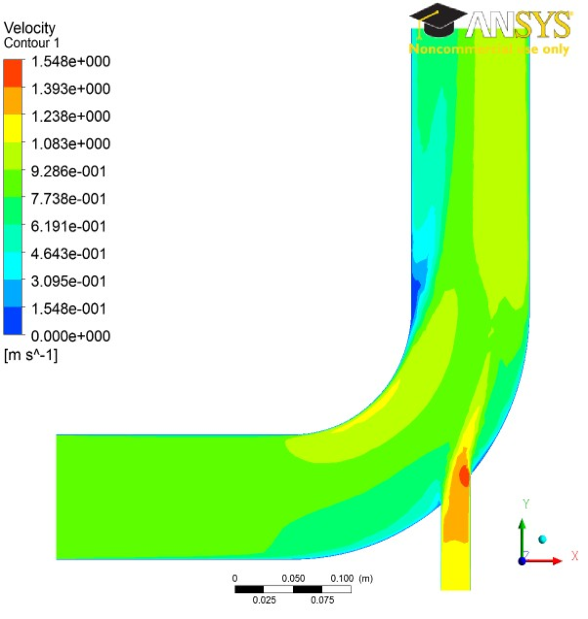
\includegraphics{provided_instructions/background/5e1-1.pdf}
%       \caption{Velocity distribution on the mid-plane for an inlet velocity for case 1.}
%       \label{veldis}
% \end{figure}
% %%%%%%%%%%%%%%%%%%%%%%%%%%%%%%%%%%%%%%%%

% The figure and caption should be centred. The figure numbering starts at 1 at the beginning of each chapter. The caption should provide a brief description of what is being shown. The figure should appear in the document after it is referred to in the text. No figure should be included which is not referred to in the text. Ensure that the size and resolution of images imported from software are sufficient to read any text.

% \section{Tables}
% Tables are an important way of displaying your results. Table \ref{tab:treatments} is a sample table, adapted from the Master/Doctoral Thesis template at \url{http://www.latextemplates.com/cat/theses}, which was generated with this code:

% {\footnotesize
% \begin{verbatim}
% \begin{table}[b]
% \caption{The effects of treatments X and Y on the four groups studied.}
% \label{tab:treatments}
% \centering
% \begin{tabular}{l l l}
% \toprule
% \textbf{Groups} & \textbf{Treatment X} & \textbf{Treatment Y} \\\midrule
% 1 & 0.2 & 0.8\\
% 2 & 0.17 & 0.7\\
% 3 & 0.24 & 0.75\\
% 4 & 0.68 & 0.3\\
% \bottomrule\\
% \end{tabular}
% \end{table}
% \end{verbatim}
% }

% \begin{table}[b]
% \caption{The effects of treatments X and Y on the four groups studied.}
% \label{tab:treatments}
% \centering
% \begin{tabular}{l l l}
% \toprule
% \textbf{Groups} & \textbf{Treatment X} & \textbf{Treatment Y} \\
% \midrule
% 1 & 0.2 & 0.8\\
% 2 & 0.17 & 0.7\\
% 3 & 0.24 & 0.75\\
% 4 & 0.68 & 0.3\\
% \bottomrule\\
% \end{tabular}
% \end{table}

% Tables are numbered in the same way as figures. Typically tables also have a short caption, but this is not universally true. The number and caption appear above the table, not below as with figures. Again, no table should appear in the report which has not been referred to in the text. Tables should come after they are discussed in the text. The exact formatting of the table depends somewhat on the content of the table, but in general, the text in the table should be the same font and size as the main text. 

% \section{Equations}
% All equations should be numbered sequentially. The numbering restarts automatically at the beginning of each chapter, and contains the number of the chapter alongside the equation number. Unlike figures and tables, you may not need to refer to every equation in the text. You should take care to format equations properly. Do no simply try to use plain text. Use the equation layout facilities. An example of how equations should appear is shown in \eqref{sampleequation}. Here is the code for it:

% {\footnotesize
% \begin{verbatim}
% \begin{equation}
% \textrm{div}(\underline{u}) = \frac{\delta u}{\delta x} + \frac{\delta v}{\delta y} +
%         \frac{\delta w}{\delta z} = 0
% \label{sampleequation}
% \end{equation} 
% \end{verbatim}
% }

% \begin{equation}
% \textrm{div}(\underline{u}) = \frac{\delta u}{\delta x} + \frac{\delta v}{\delta y} + \frac{\delta w}{\delta z} = 0
% \label{sampleequation}
% \end{equation} 

% \section{Referencing published work}
% It is important to give appropriate credit to other people for the work that they have shared through publications. In fact, you must sign a declaration in your report stating that you understand the nature of plagiarism. As well as avoiding plagiarism, citing results or data from the literature can strengthen your argument, provide a favourable comparison for your results, or even demonstrate how superior your work is.

% There are many styles to reference published work. For example, the parenthetical style (which is also called the \emph{Harvard style}) uses the author and date of publication (e.g. ``Smith and Jones, 2001''). There is also the Vancouver style (or the \emph{citation sequence style}). In the IEEE style, which is used in this document in the default setup, the publications are cited using bracketed numbers which refer to the list in the References section at the end of the report. The references are listed in the order that they are cited in the report. A variant is \emph{name sequence style}, in which the publications are referenced by number, but the list is arranged alphabetically. The following paragraph shows the use of the IEEE style: 

% \begin{quote}
% Several studies have examined the sound field around tandem cylinders generated by flow cite{fitzpatrick2003flow,finnegan2010experimental}, while other investigations have focused on the effect of an applied sound field on the flow cite{hall2003vortex}. Papers from conference proceedings cite{jordan2001array}, books cite{paidoussis2010fluid} and technical reports cite{reyes2007power} can be dealt with in the same style.
% \end{quote}

% The IEEE style has the advantage that it is a little more compact in the text and does not distract from the flow of the sentence if there are a lot of citations. However, it has the disadvantage that it is not immediately clear to the reader what particular work has been referenced. You can use author names directly and discuss the work of Finnegan et al. cite{finnegan2010experimental} similar to this sentence to make it more readable. 

% It actually does not matter which particular referencing style is used as long as three important considerations are observed:
% \begin{itemize}
% \item the referencing style used throughout the document is consistent;
% \item all material used or discussed in the text is properly cited;
% \item nothing is included in the reference list that has not been cited.
% \end{itemize}

% Check with your supervisor as they may have a strong opinion on what you should use

% This template has a suitable referencing style already set up -- you should use it and use the built-in BibTeX system to manage your references. See above for examples of how to cite a reference and look in the \texttt{sample.bib} file to see BibTeX references. It is strongly recommended that you use a bibliographic tool, such as EndNote (check out https://www.tcd.ie/library/support/endnote/), as this will facilitate compliance with these three requirements. Endnote can help you build you .bib file. Remember \href{http://scholar.google.com}{Google Scholar} and other search engines will give you BibTeX references for lots of academic publications. Be aware that Web of Science is more reliable for giving the full record for the BibTeX entry. Otherwise, you can easily make up your own based on the examples in that file.
% \chapter{\LaTeX (Remove from Final)}
% \label{latexchapter}
% \textsc{\LARGE \underline{REMOVE FROM FINAL SUBMISSION}}

% \LaTeX{}, or more properly ``\LaTeXe{}'', is a very useful document processing program. It is very widely used, widely available, stable and free. Famously, \TeX, upon which \LaTeX{} is built, was originally developed by the eminent American mathematician Donald Knuth because he was tired of ugly mathematics books cite{shustek2008interview}. Although it has a learning curve (made much less forbidding by online tools and resources -- see below), it allows the writer to concentrate more fully on the content, and takes care of most everything else.

% While it can be used as a word processor, it is a \emph{typesetting} system, and Knuth's idea was that it could be used to produce beautiful looking books:
% \begin{quote}
% \emph{\LaTeX{} is a macro package which enables authors to typeset and print their work at the highest typographical quality, using a predefined, professional layout.}\footnote{This is from cite{oetiker2001not}. Did we mention that you should minimise your use of footnotes?}
% \end{quote}
% \LaTeX{} has great facilities for setting out equations and a powerful and very widely supported bibliographic system called BibTeX, which takes the pain out of referencing.

% Three useful online resources make \LaTeX~much better:
% \begin{enumerate}[(1)]
% \item An excellent online \LaTeX{} environment called ``Overleaf'' is available at \url{http://www.overleaf.com} and runs in a modern web browser. It's got this template available -- search for a TCD template. Overleaf can work in conjunction with Dropbox, Google Drive and, in beta, GitHub.
% \item Google Scholar, at \url{http://scholar.google.com}, provides BibTeX entries for most of the academic references it finds.
% \item An indispensable and very fine introduction to using \LaTeX{} called \emph{``The not so short introduction to LATEX 2$\varepsilon$''} by cite{oetiker2001not} is online at \url{https://doi.org/10.3929/ethz-a-004398225}. Browse it before you use \LaTeX~for the first time and  read it carefully when you get down to business.
% \end{enumerate}
% Other tools worth mentioning include:
% \begin{itemize}
% \item \texttt{Draw.io} -- an online drawing package that can output PDFs to Google Drive -- see \url{https://www.draw.io}.
% \end{itemize}

% note that your supervisor may have a strong opinion on the style of referencing you use. Some background is available at https://www.overleaf.com/learn/latex/Bibtex_bibliography_styles
\bibliographystyle{IEEEtran} %Changed to IEEETran by HS
%\bibliographystyle{unsrt}

\appendix
\renewcommand{\thechapter}{A\arabic{chapter}}
%% \chapter{Appendix Instructions (Remove from Final)}
% You may use appendices to include relevant background information, such as calibration certificates, derivations of key equations or presentation of a particular data reduction method. You should not use the appendices to dump large amounts of additional results or data which are not properly discussed. If these results are really relevant, then they should appear in the main body of the report.

% \section{Appendix numbering}
% Appendices are numbered sequentially, A1, A2, A3\ldots The sections, figures and tables within appendices are numbered in the same way as in the main text. For example, the first figure in Appendix A1 would be Figure A1.1. Equations continue the numbering from the main text.

\chapter{Figures \& Data}
\label{appendix_layers_figures}
\section{Results for Increasing Numbers of Layers}
\subsection{\texorpdfstring{\acrshort{uav}}{UAV} Trajectory}
\begin{figure} [ht!]
    \centering
    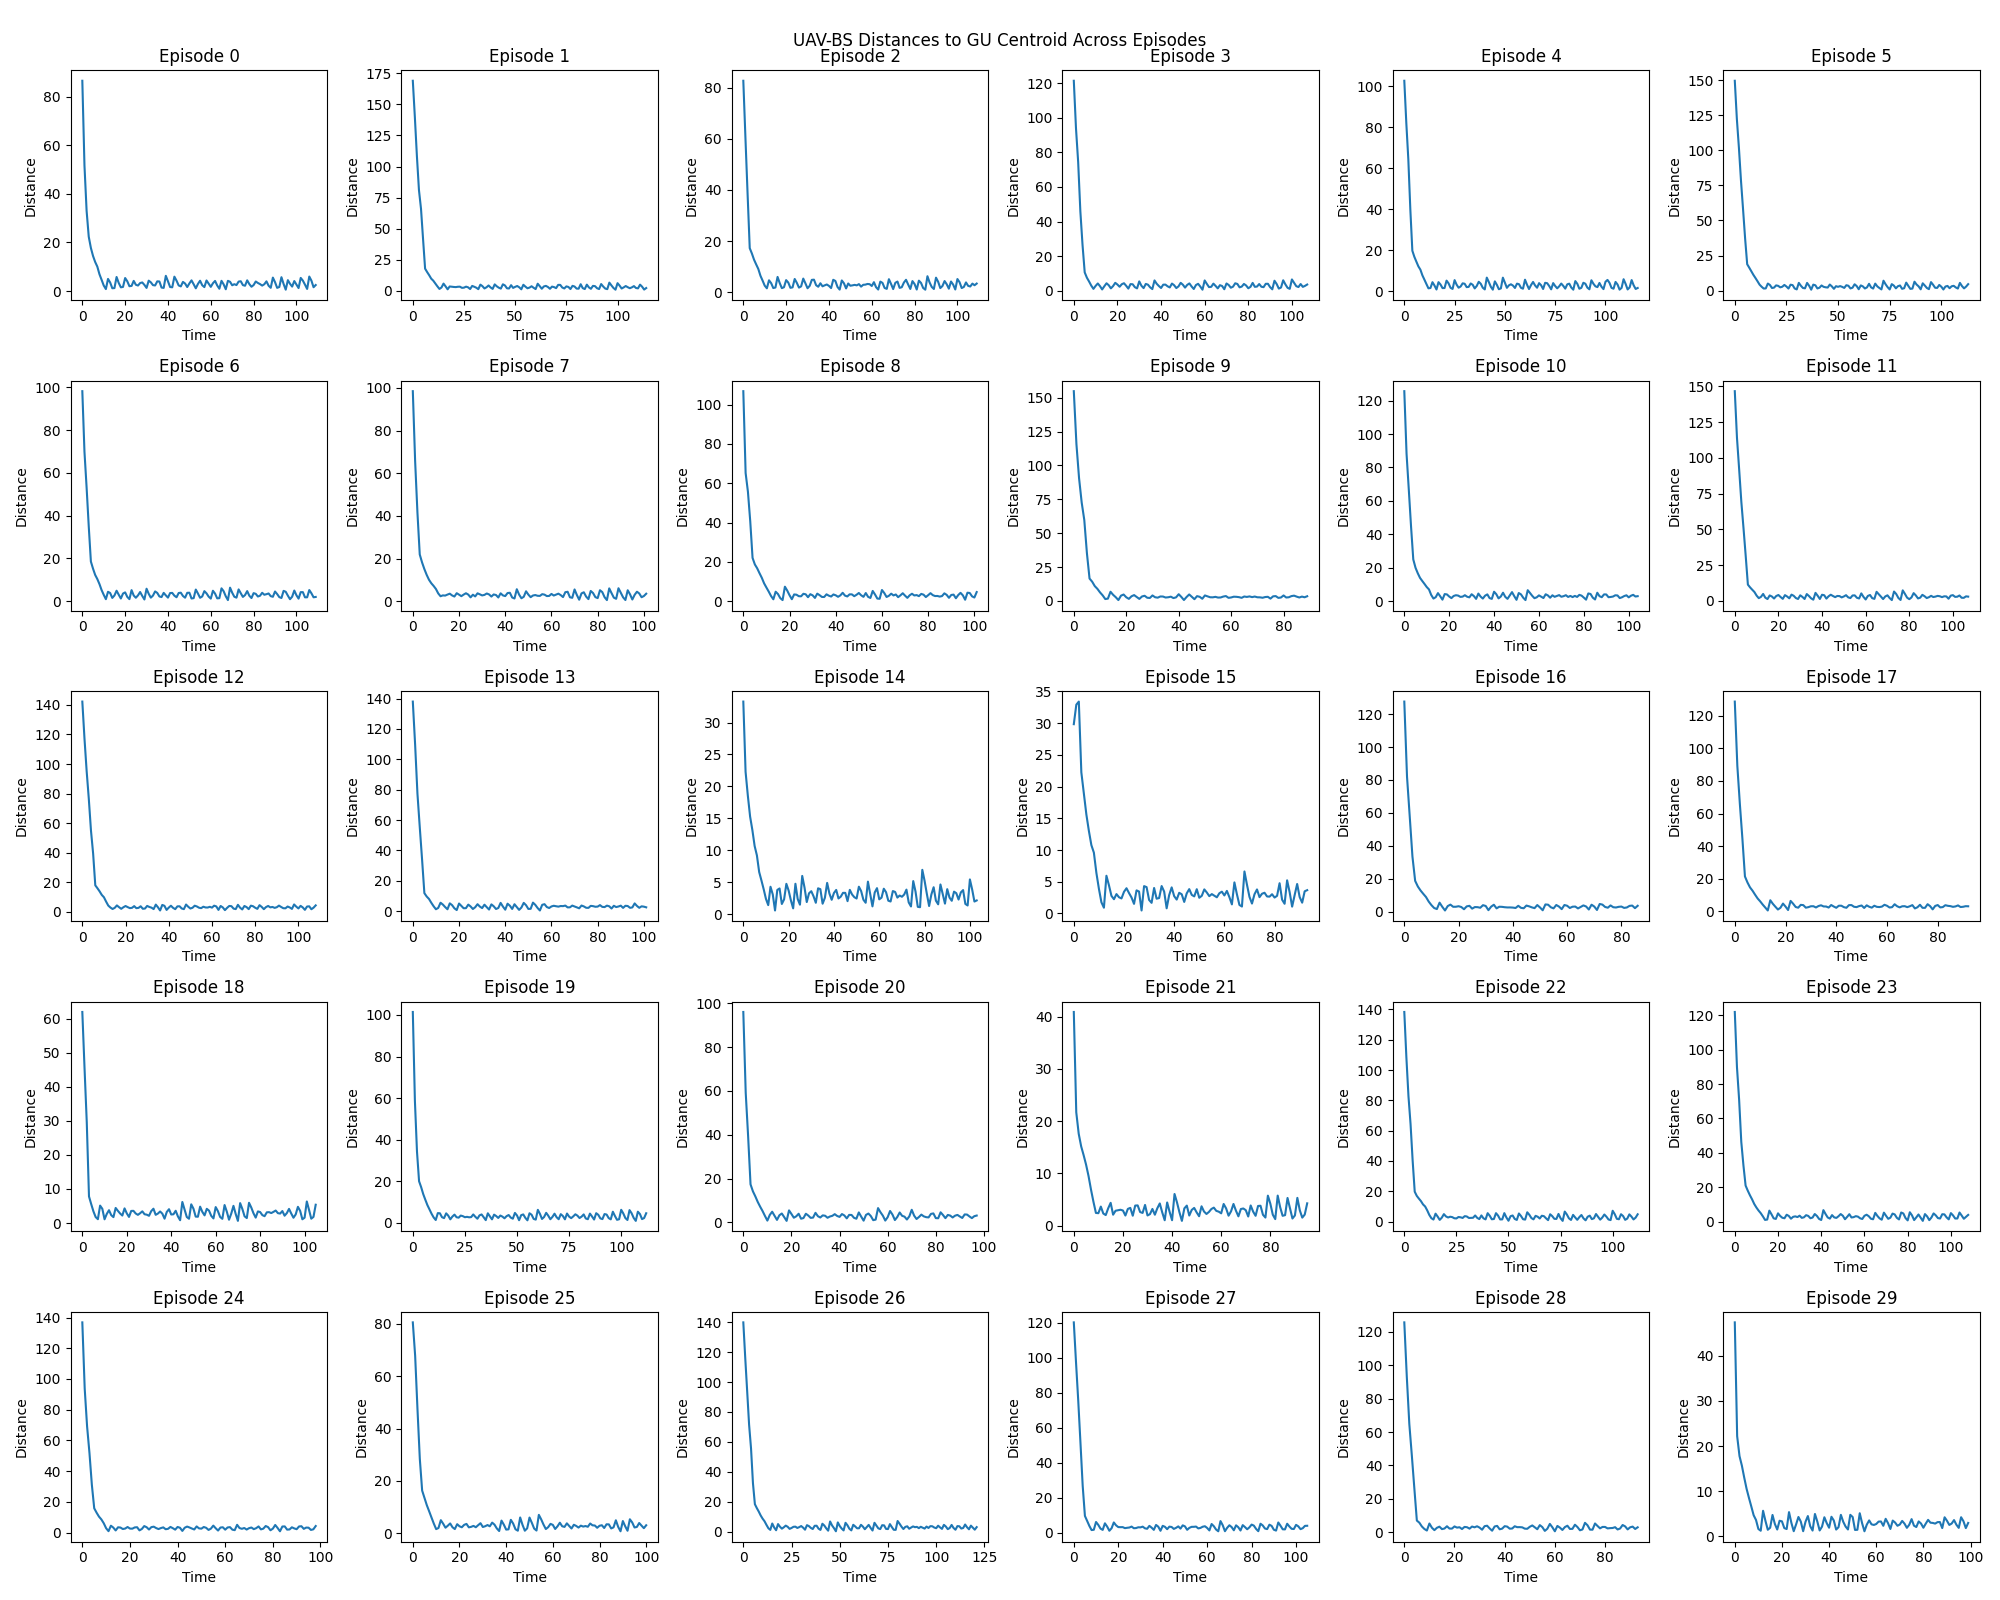
\includegraphics[width=0.8\linewidth]{figures/test8_without_trajectory/1_layers_distances_to_centroid.png}
    \caption{Max, Min \& Mean Distances to Centroid Across 30 Episodes for M = 1}
    \label{fig:dist_to_centroid_1_layer_30_ep}
\end{figure}
\begin{figure}
    \centering
    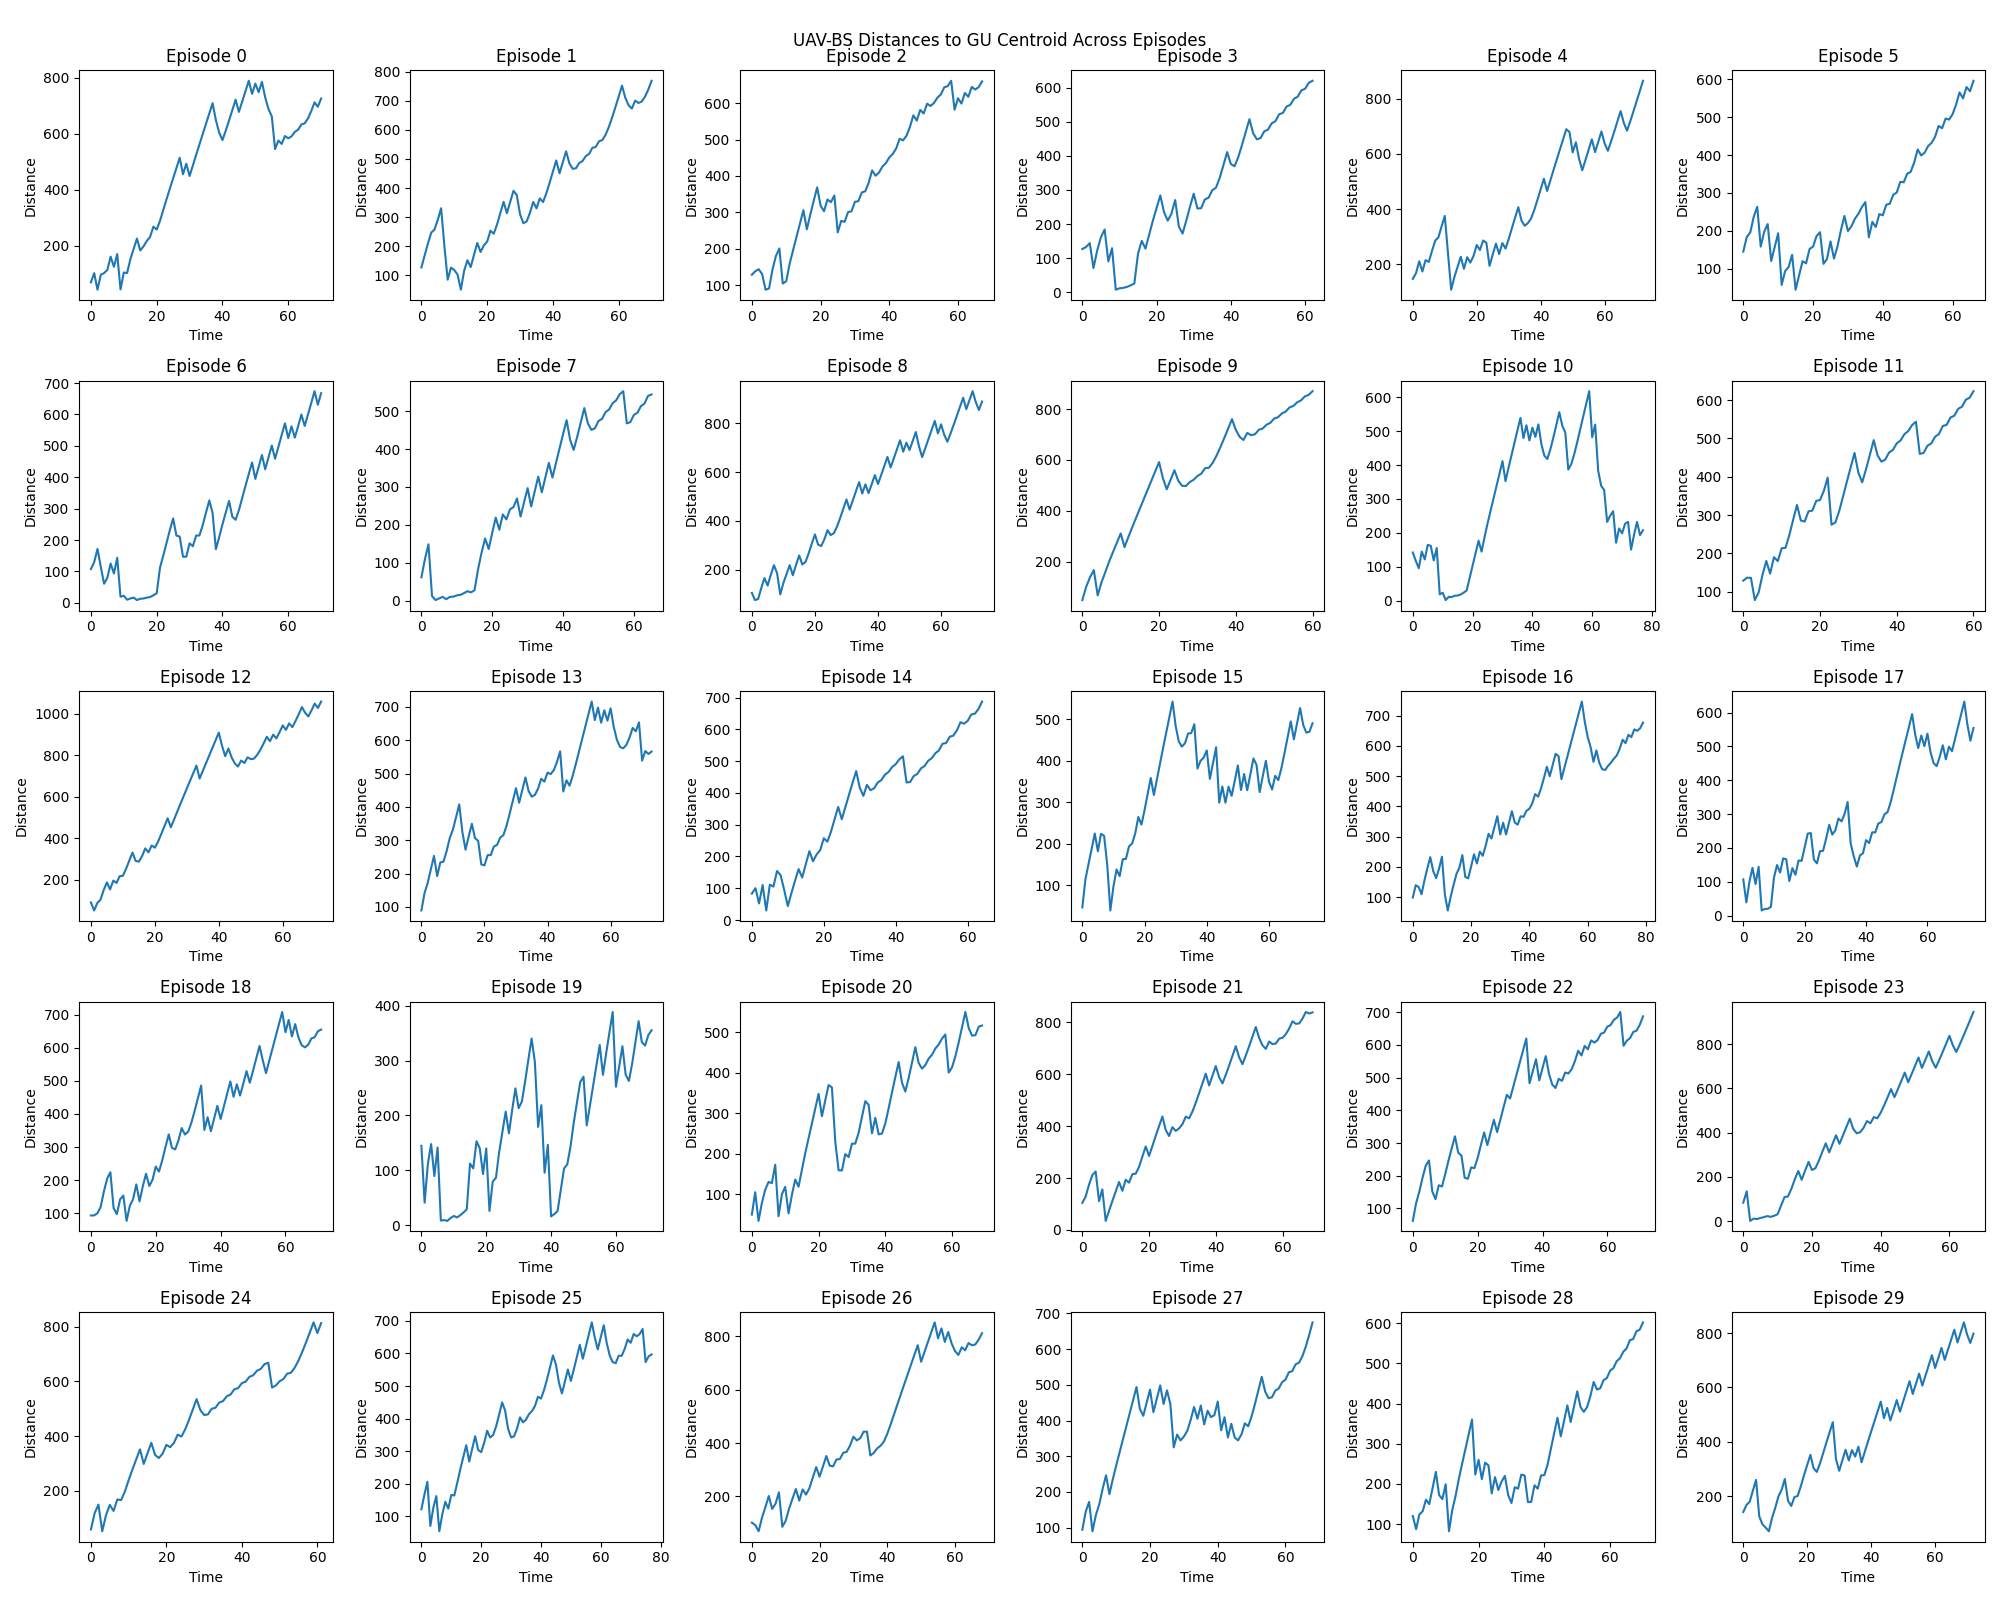
\includegraphics[width=0.8\linewidth]{figures/test8_without_trajectory/2_layers_distances_to_centroid.png}
    \caption{Max, Min \& Mean Distances to Centroid Across 30 Episodes for M = 2}
    \label{fig:dist_to_centroid_2_layers_30_ep}
\end{figure}
\begin{figure}
    \centering
    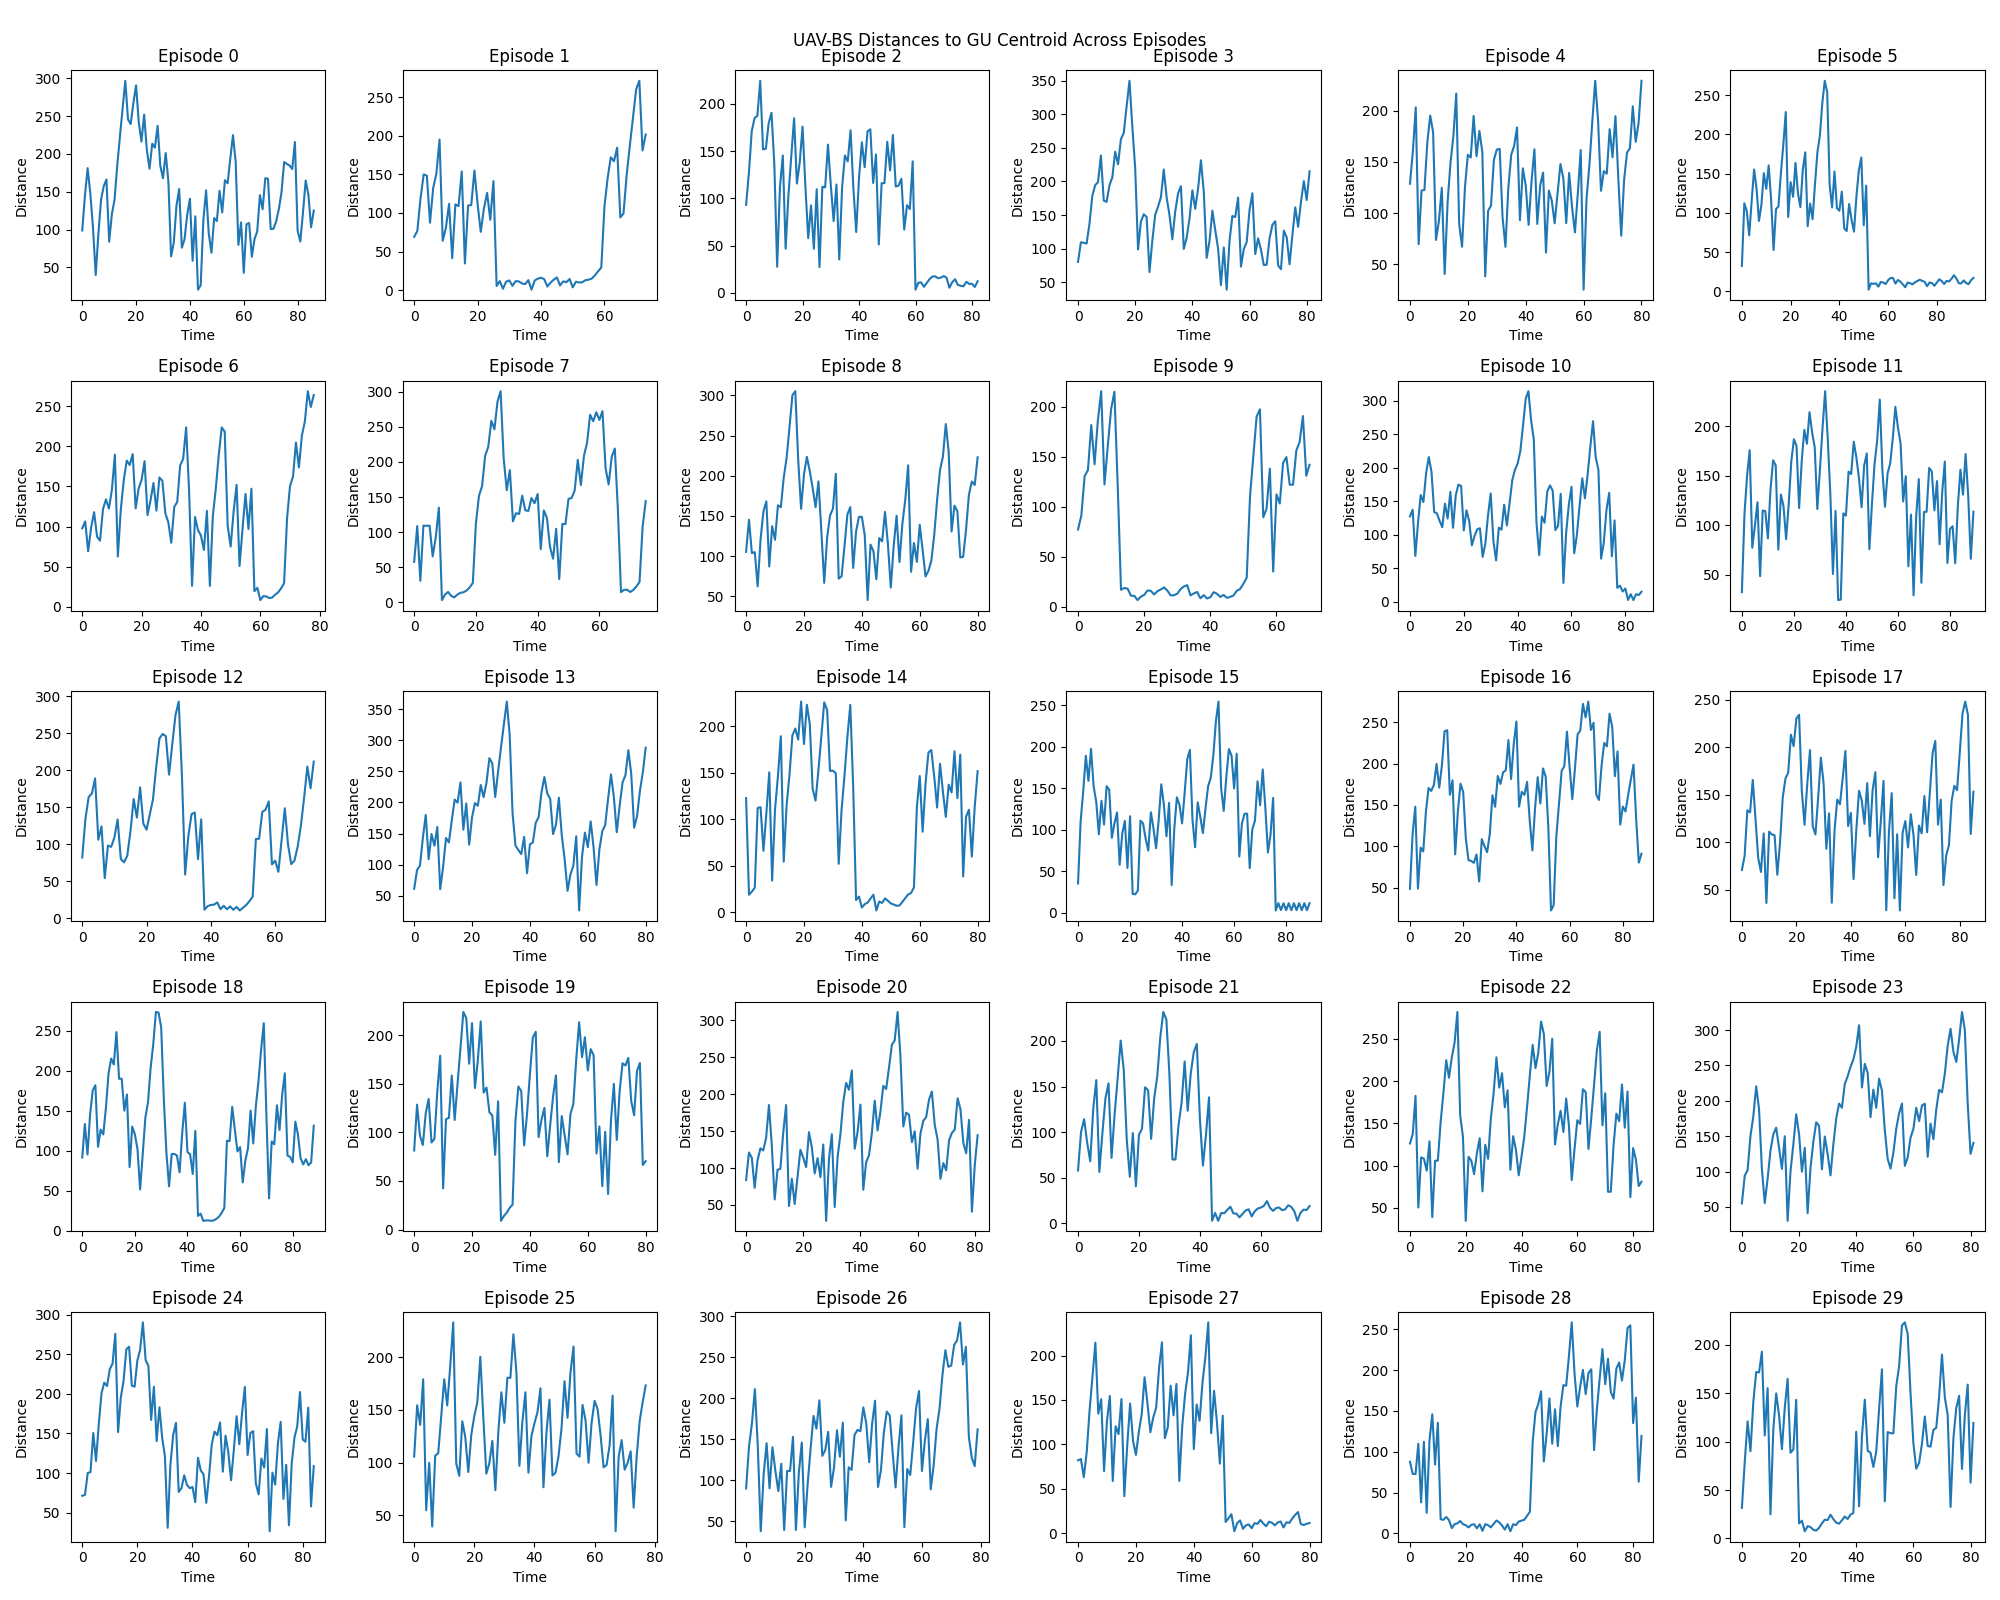
\includegraphics[width=0.8\linewidth]{figures/test8_without_trajectory/3_layers_distances_to_centroid.png}
    \caption{Max, Min \& Mean Distances to Centroid Across 30 Episodes for M = 3}
    \label{fig:dist_to_centroid_3_layers_30_ep}
\end{figure}
\begin{figure}
    \centering
    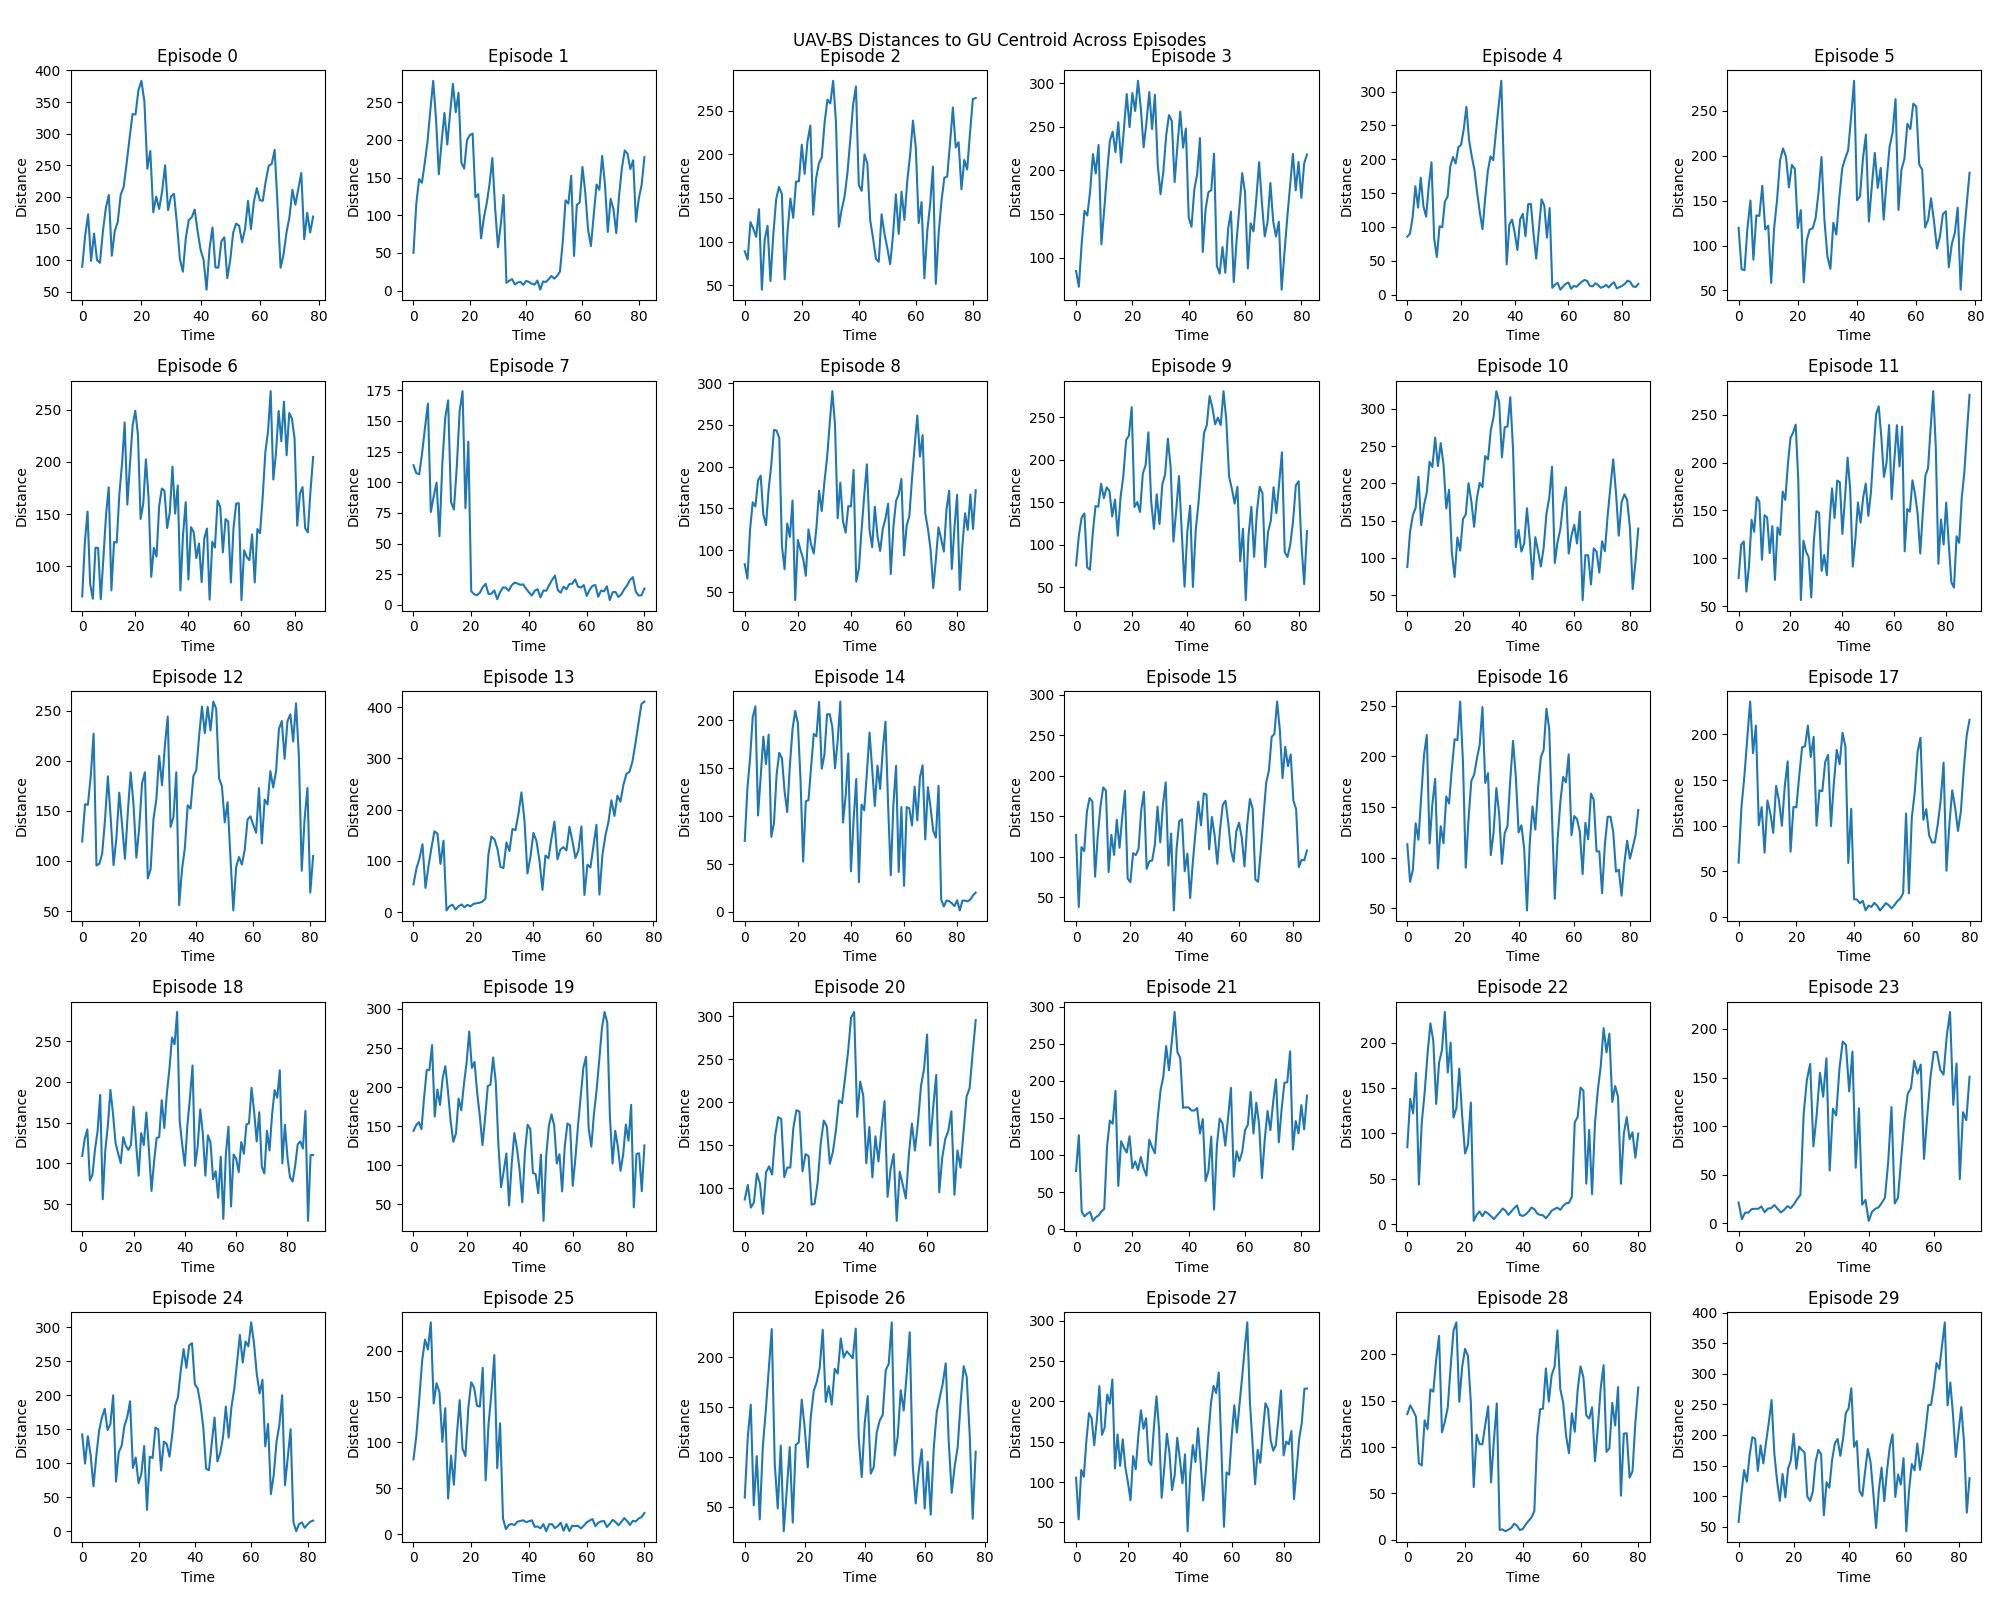
\includegraphics[width=0.8\linewidth]{figures/test8_without_trajectory/4_layers_distances_to_centroid.png}
    \caption{Max, Min \& Mean Distances to Centroid Across 30 Episodes for M = 4}
    \label{fig:dist_to_centroid_4_layers_30_ep}
\end{figure}
\begin{figure}
    \centering
    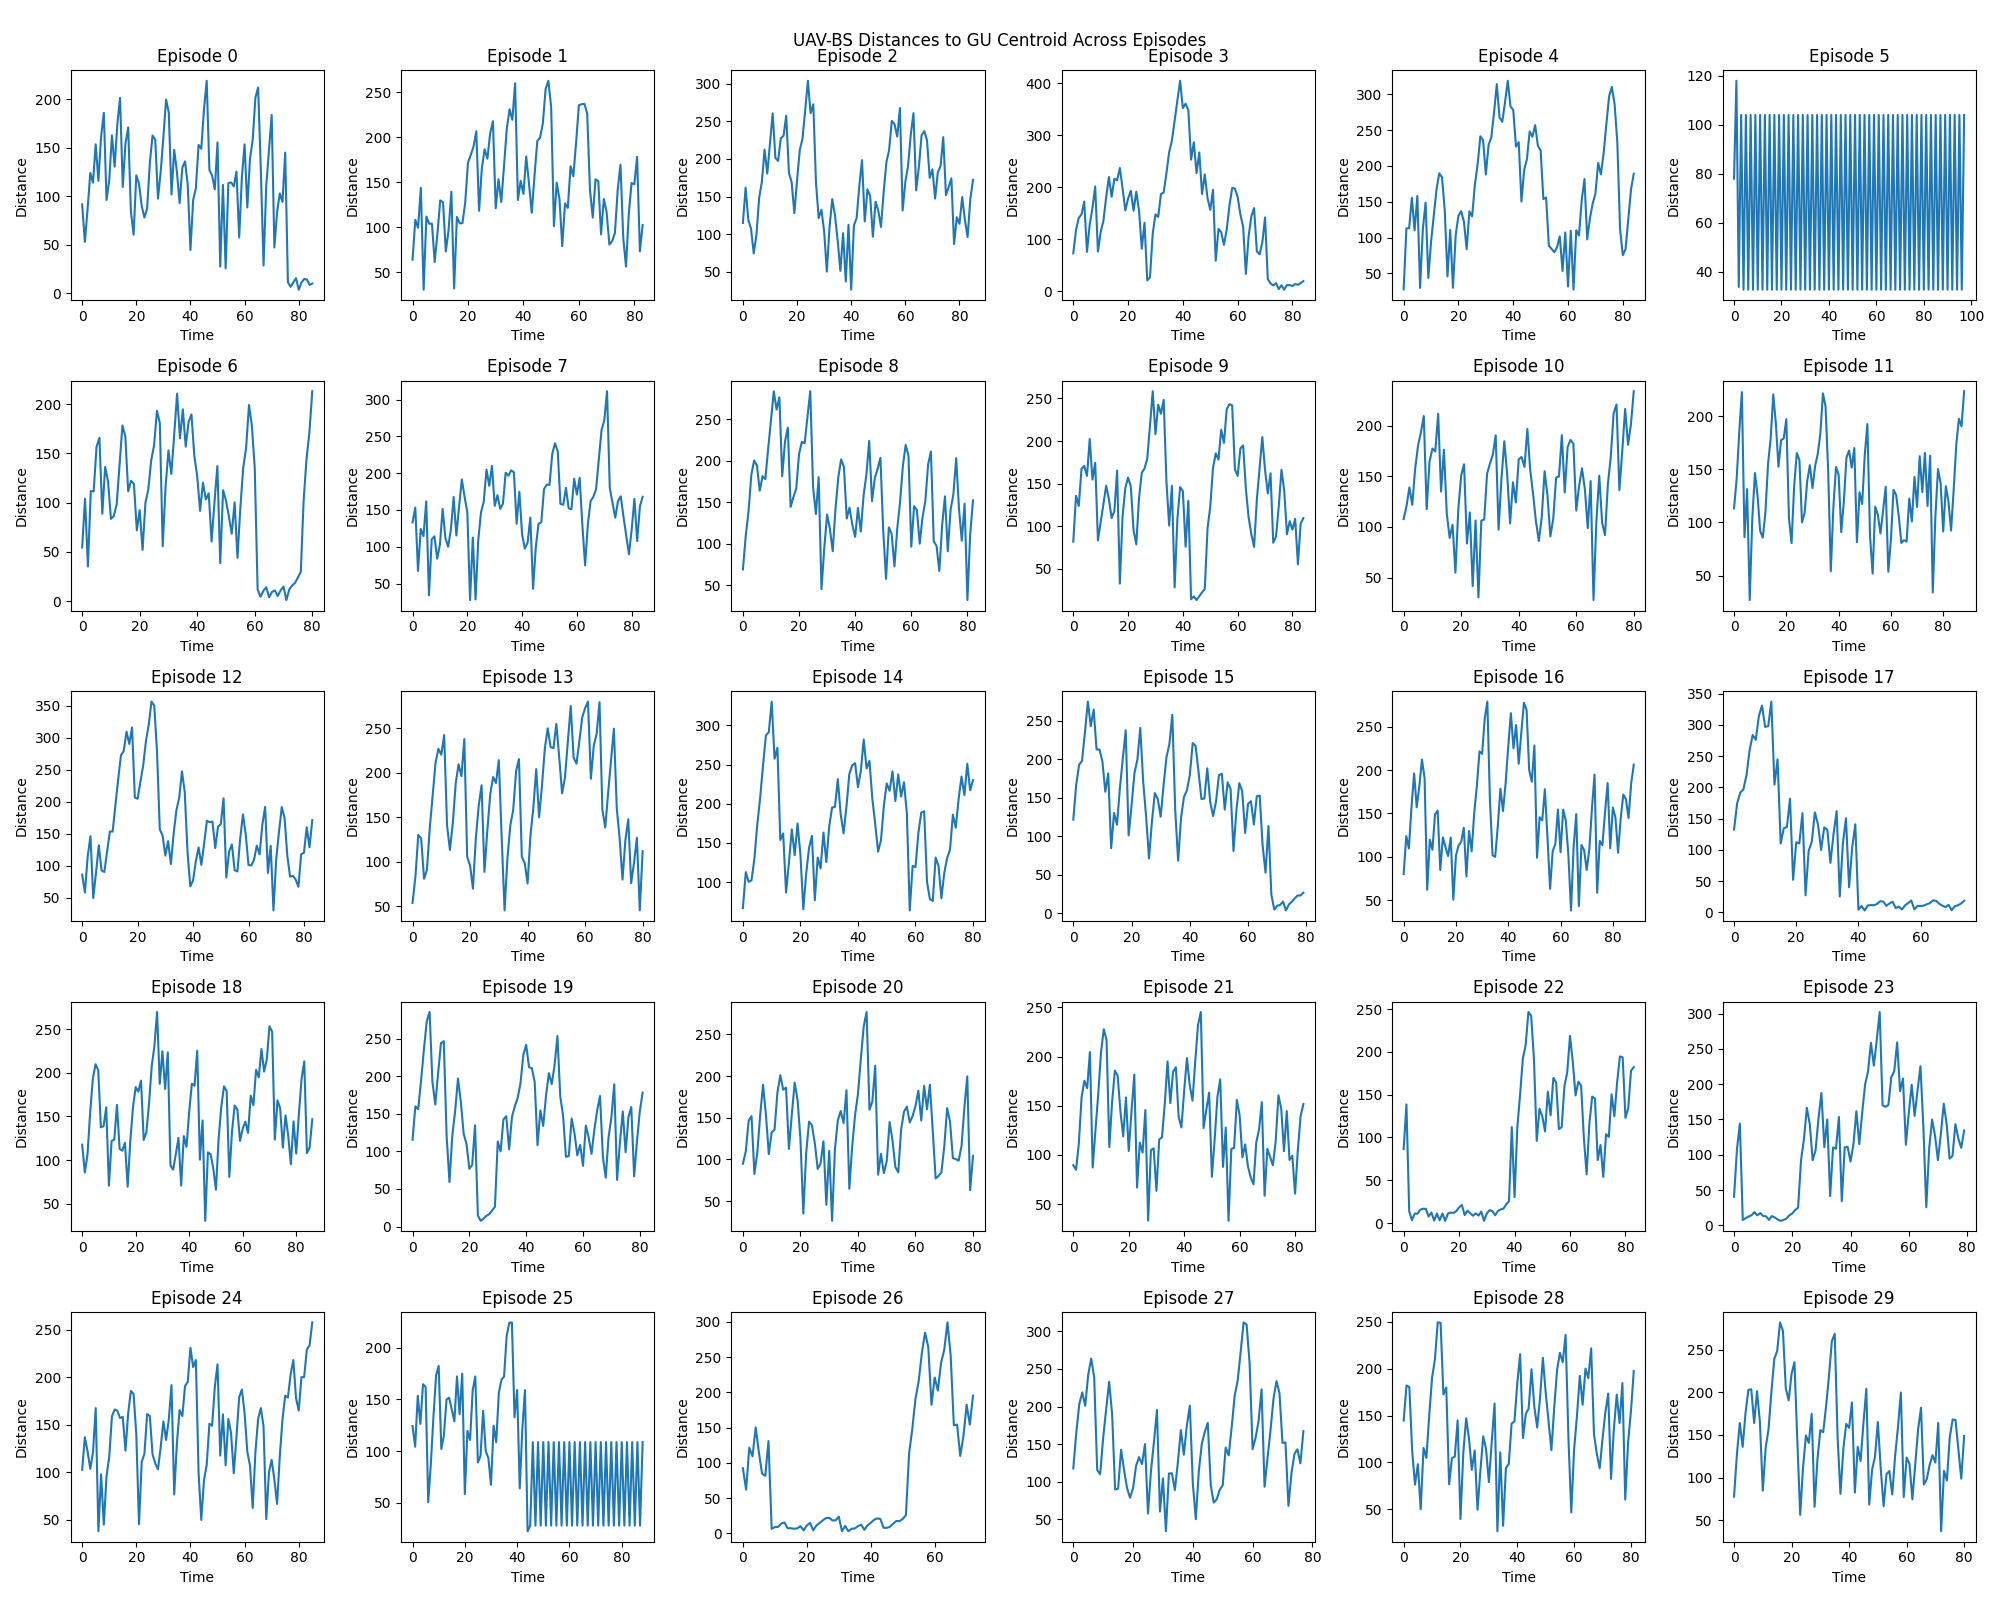
\includegraphics[width=0.8\linewidth]{figures/test8_without_trajectory/5_layers_distances_to_centroid.png}
    \caption{Max, Min \& Mean Distances to Centroid Across 30 Episodes for M = 5}
    \label{fig:dist_to_centroid_5_layers_30_ep}
\end{figure}
\newpage
\subsection{Data Exchange Rate}
\begin{figure} [ht!]
    \centering
    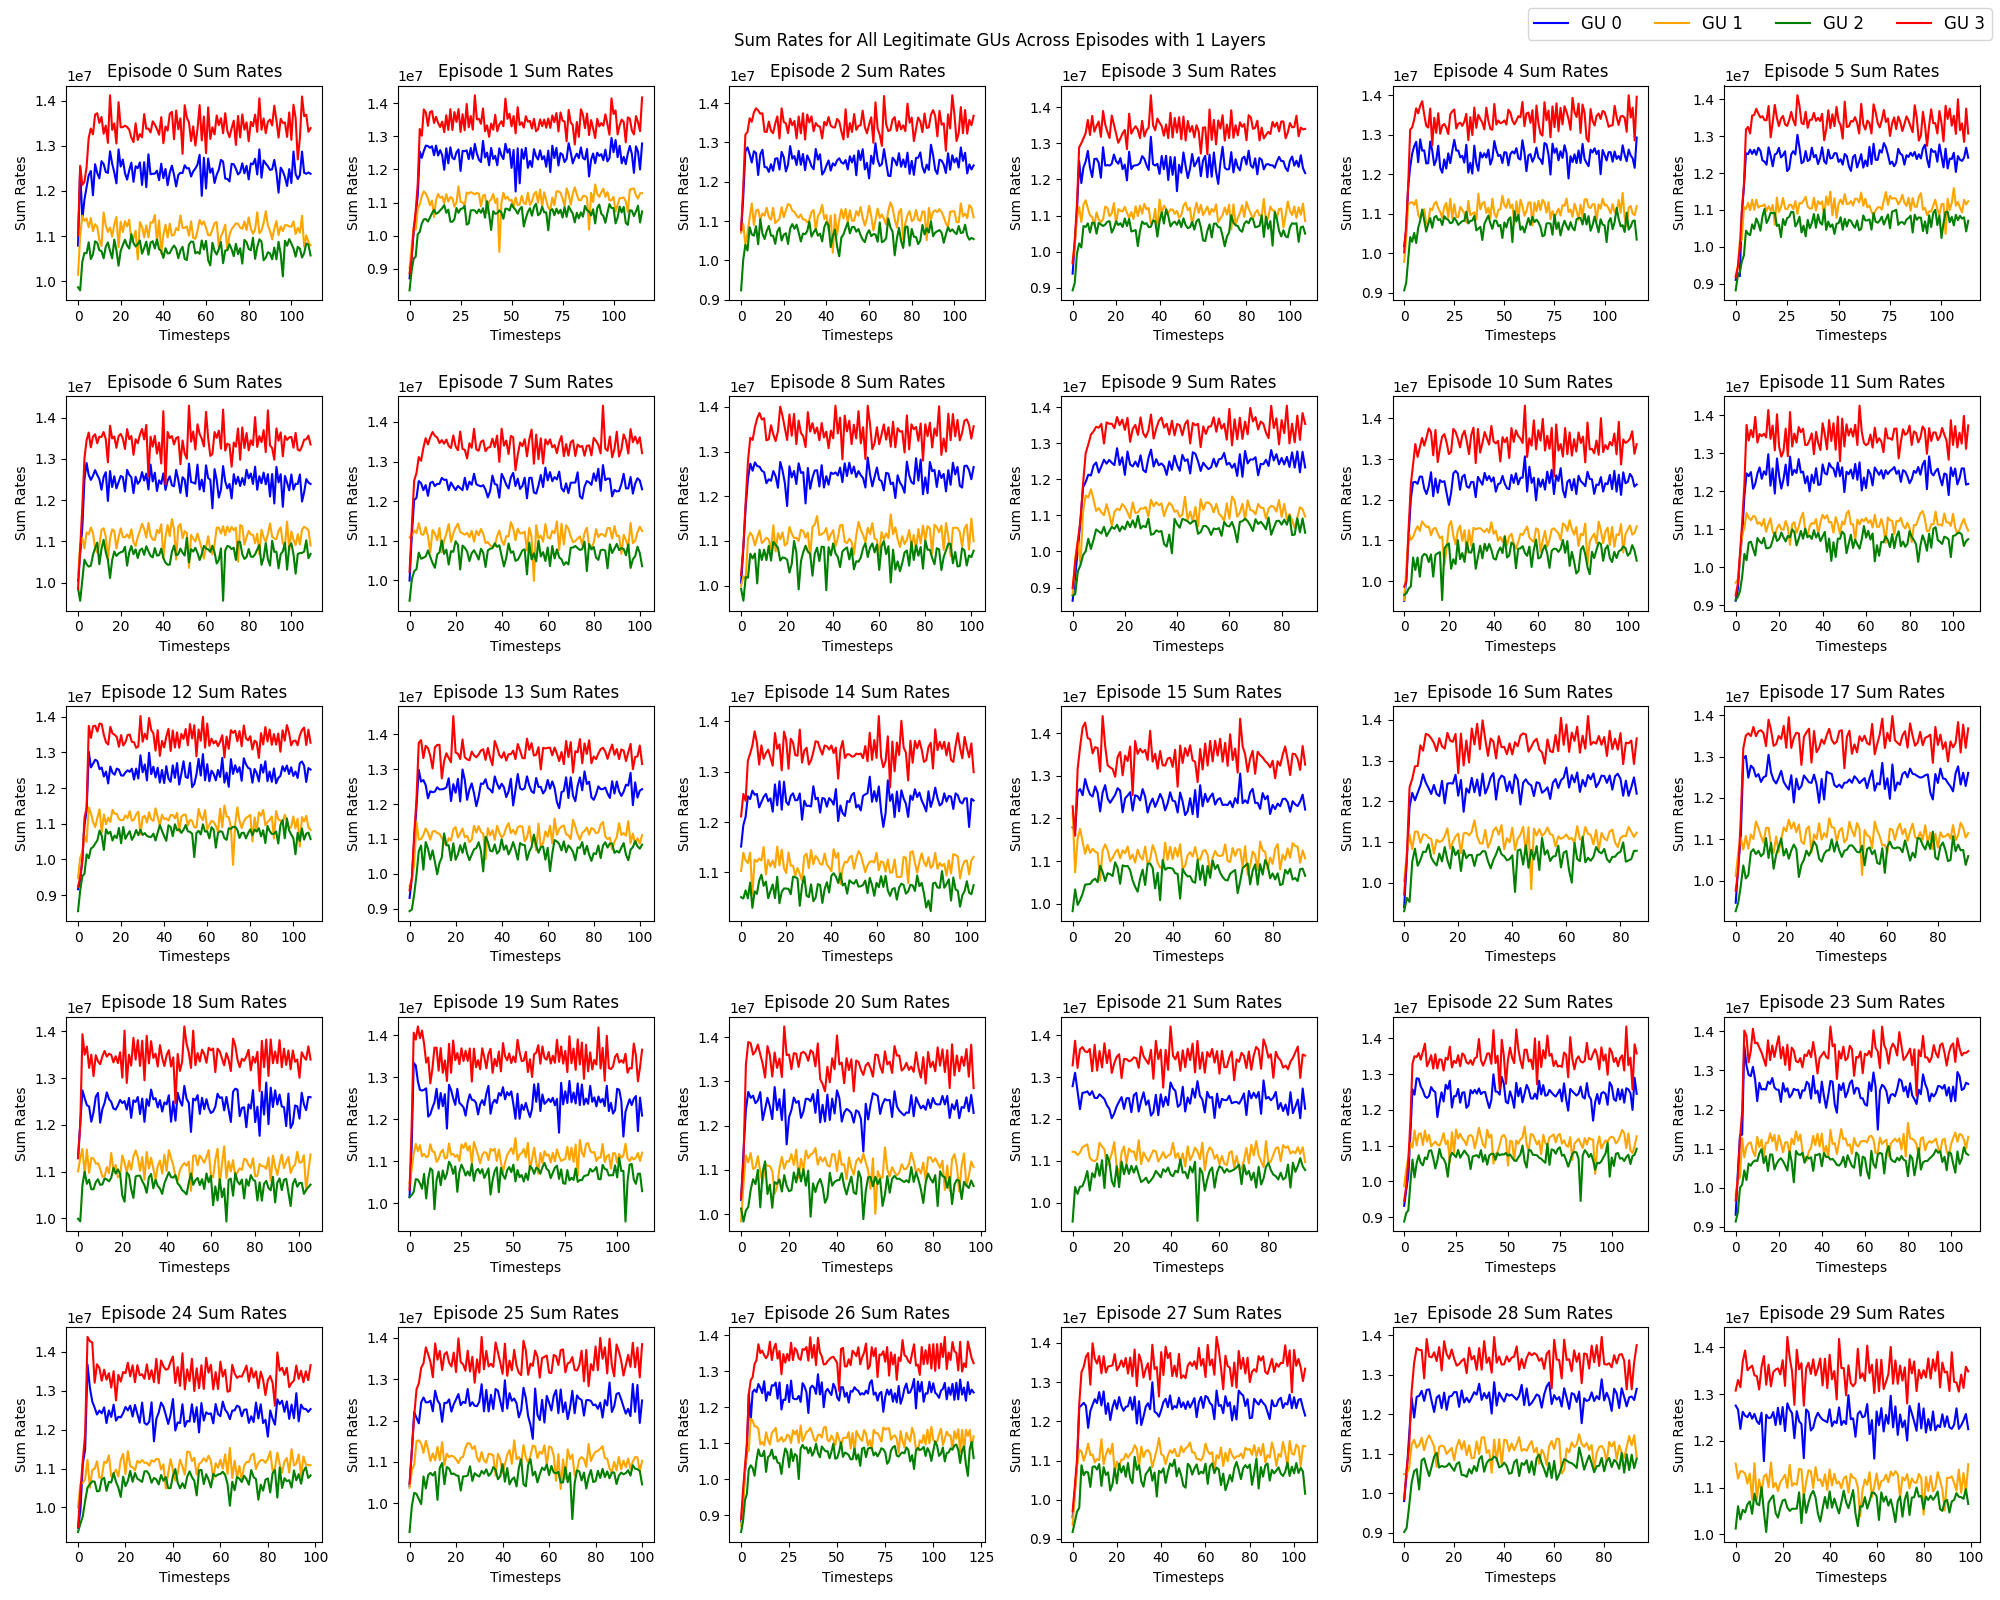
\includegraphics[width=0.8\linewidth]{figures/test8_without_trajectory/1_layers_sum_rates.png}
    \caption{Max, Min \& Mean Data Exchange Rates Across 30 Episodes for M = 1}
    \label{fig:data_rate_1_layer_30_ep}
\end{figure}
\begin{figure}
    \centering
    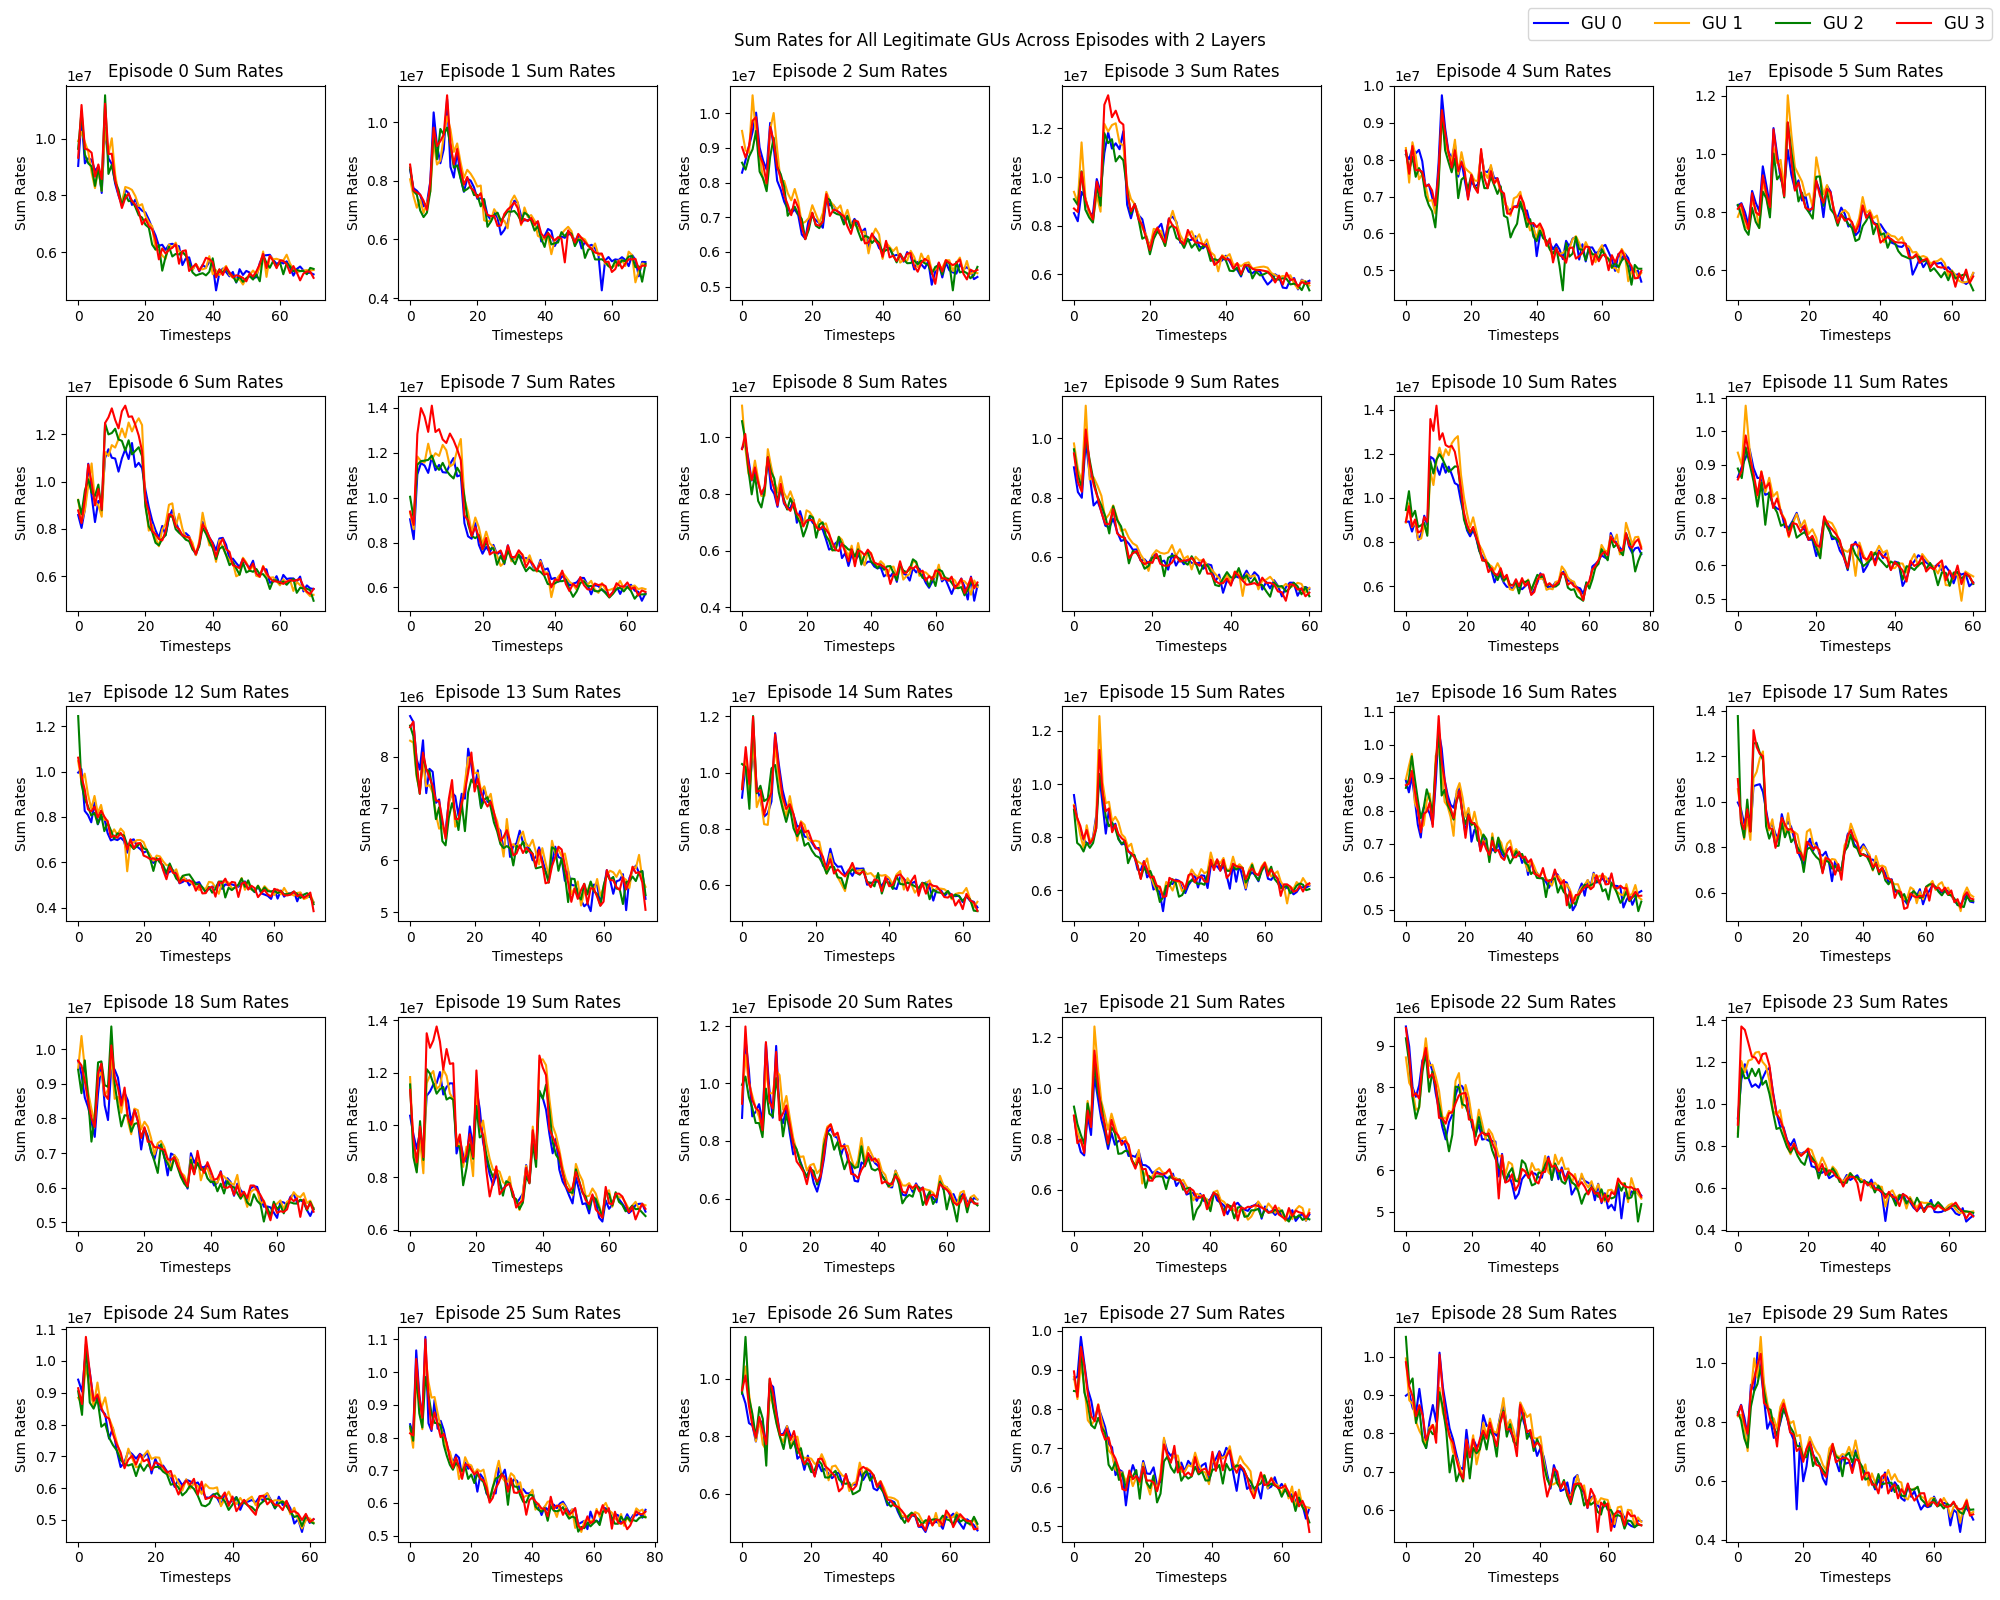
\includegraphics[width=0.8\linewidth]{figures/test8_without_trajectory/2_layers_sum_rates.png}
    \caption{Max, Min \& Mean Data Exchange Rates Across 30 Episodes for M = 2}
    \label{fig:data_rate_2_layers_30_ep}
\end{figure}
\begin{figure}
    \centering
    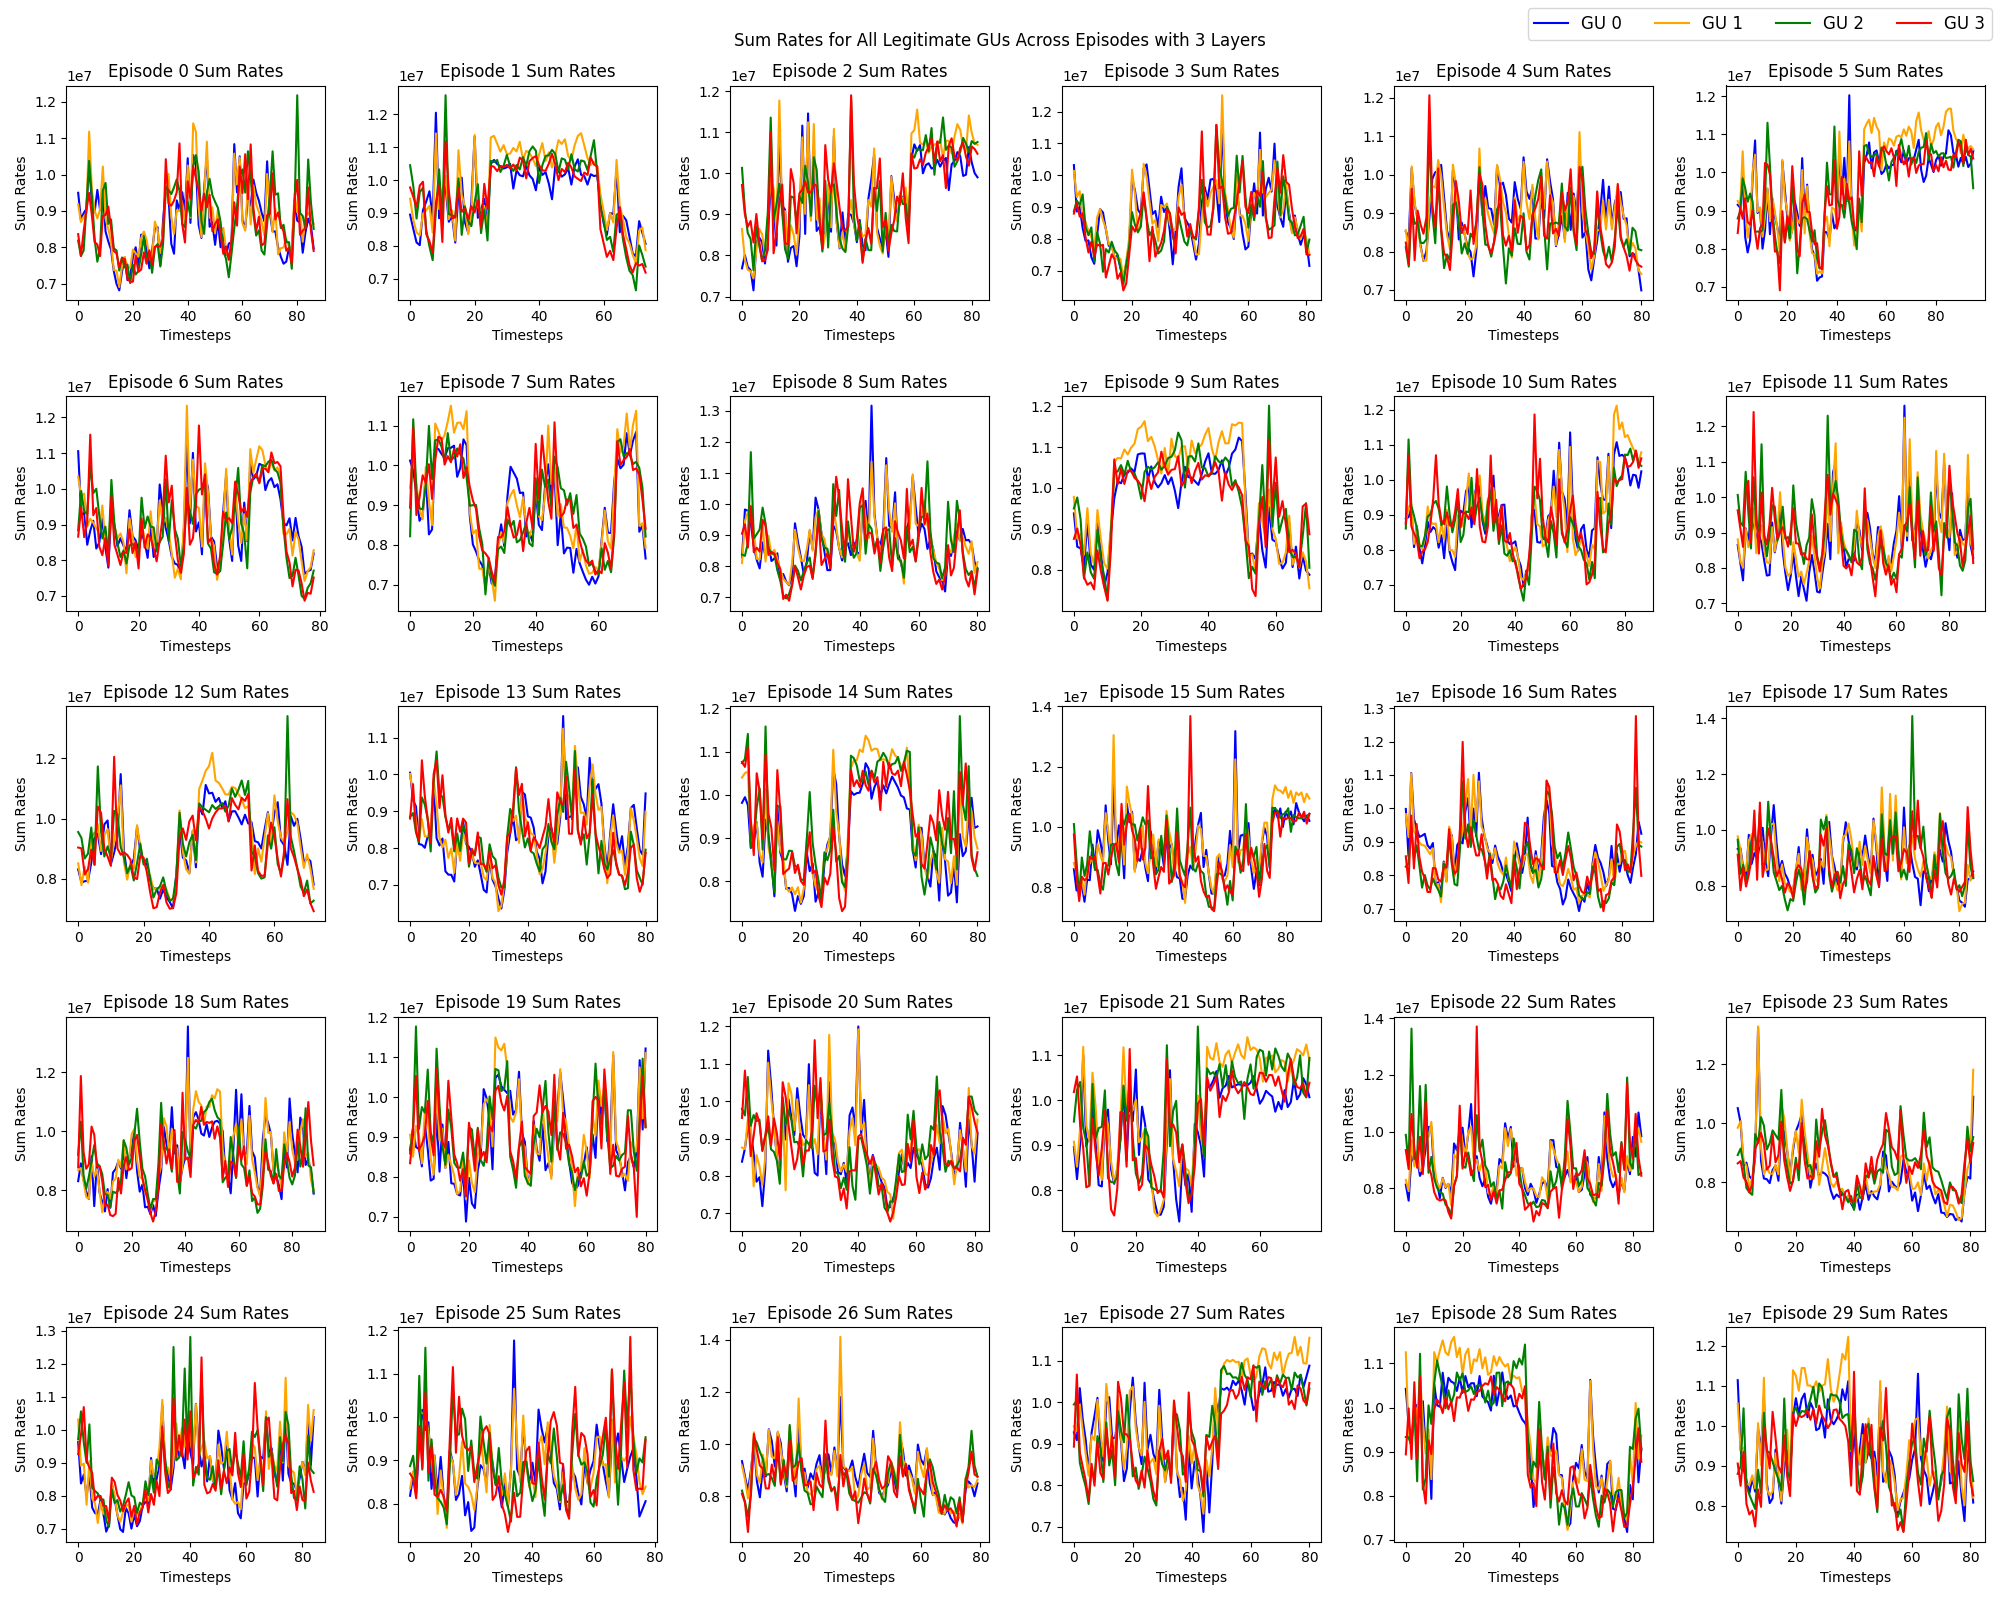
\includegraphics[width=0.8\linewidth]{figures/test8_without_trajectory/3_layers_sum_rates.png}
    \caption{Max, Min \& Mean Data Exchange Rates Across 30 Episodes for M = 3}
    \label{fig:data_rate_3_layers_30_ep}
\end{figure}
\begin{figure}
    \centering
    \includegraphics[width=0.8\linewidth]{figures/test8_without_trajectory/4_layers_sum_rates.png}
    \caption{Max, Min \& Mean Data Exchange Rates Across 30 Episodes for M = 4}
    \label{fig:data_rate_4_layers_30_ep}
\end{figure}
\begin{figure}
    \centering
    \includegraphics[width=0.8\linewidth]{figures/test8_without_trajectory/5_layers_sum_rates.png}
    \caption{Max, Min \& Mean Data Exchange Rates Across 30 Episodes for M = 5}
    \label{fig:data_rate_5_layers_30_ep}
\end{figure}


\end{document}